\documentclass[12pt,a4paper,final]{report}

\usepackage{pdfpages}
\usepackage{fancyhdr}
\usepackage{amsmath}
\usepackage{graphicx}
\usepackage[hidelinks]{hyperref}
\usepackage{geometry}
\usepackage{setspace}
\usepackage{bookmark}
\usepackage{titlesec}
\usepackage{datatool}
\usepackage{tikz}
\usepackage{textcomp} % For \MakeUppercase
\usepackage[backend=bibtex, style=numeric]{biblatex}
\usepackage{glossaries} % For creating an index of abbreviations
\usepackage{longtable} % For tables that span multiple pages
\usepackage{xcolor}
\usepackage{subcaption} % for subfigures
\usepackage{pgfplots}
\usepackage{pgfplotstable}
\usepackage{multirow}
\usepackage{comment}  % Load the comment package
\usepackage{placeins}  % Add this to the preamble

\pgfplotsset{compat=1.17}

% for creating diagrams and flowcharts
\usetikzlibrary{shapes.geometric, arrows, positioning}

% Define a custom dark green color
\definecolor{darkgreen}{rgb}{0.0, 0.5, 0.0}

\tikzstyle{startstop} = [ellipse, minimum width=1cm, minimum height=1cm, text centered, draw=black, fill=none, text width=1.5cm, line width=1pt, inner sep=0pt]
\tikzstyle{nodepage} = [circle, minimum width=0.25cm, minimum height=0.25cm, text centered, draw=black, fill=none, text width=0.5cm, line width=1pt, inner sep=0pt]
\tikzstyle{process} = [rectangle, minimum width=3cm, minimum height=1cm, text centered, draw=black, fill=none, text width=5cm]
\tikzstyle{processorange} = [trapezium, minimum width=2cm, minimum height=1cm, text centered, draw=black, fill=none, text width=5cm, line width=1pt, trapezium left angle=60, trapezium right angle=120]
\tikzstyle{decision} = [diamond, aspect=1.5, minimum width=1cm, minimum height=1cm, text centered, draw=black, fill=none, text width=3.5cm, line width=1pt, inner xsep=0cm, inner ysep=0cm]
\tikzstyle{coordinate} = [circle, minimum size=1pt, fill=black, inner sep=0pt]
\tikzstyle{arrow} = [thick,-latex,>=stealth]

% Specify line-spacing to 1.5
\onehalfspacing

% Specify margin
\geometry{top=2.5cm,bottom=2.5cm,left=3cm,right=2cm,headheight=14.5pt}

% Adjust \chapter margins
\titlespacing*{\chapter}{0pt}{0pt}{10pt} % Adjust these values as needed


% Add header and footer
\pagestyle{fancy}
\fancyhf{} % Clear all header and footer fields
% Redefine \chaptermark to remove the period after the chapter number
\renewcommand{\chaptermark}[1]{%
  \markboth{\it{\MakeUppercase{Chapter \thechapter:\ #1}}}{}}
\fancyhead[R]{\leftmark} % Left-align the chapter name
\fancyfoot[R]{Page \thepage} % Right-align page number in the footer
% Remove header line
\renewcommand{\headrulewidth}{0pt}


% Ensuring plain pages (like chapter starting pages) also use the fancy style
\fancypagestyle{plain}{
    \fancyhf{} % Clear all header and footer fields
    \fancyfoot[R]{Page \thepage} % Right-align page number in the footer
    \renewcommand{\headrulewidth}{0pt} % Remove header line on plain pages
}
\pagenumbering{Roman}

% Change Chapter formatting
\titleformat{\chapter}[hang]
    {\normalfont\huge\bfseries}
    {\thechapter}
    {1em}
    {}

% Add bibliography resources
\addbibresource{references.bib}

% Redefine \@dottedtocline to remove dots in \tableofcontents
\makeatletter
\renewcommand{\@dottedtocline}[5]{%
  \ifnum #1>\c@tocdepth \else
    \vskip \z@ \@plus.2\p@
    {\leftskip #2\relax \rightskip \@tocrmarg \parfillskip -\rightskip
     \parindent #2\relax\@afterindenttrue
     \interlinepenalty\@M
     \leavevmode
     \@tempdima #3\relax
     \advance\leftskip \@tempdima \null\nobreak\hskip -\leftskip
     {#4}\nobreak
     \leaders\hbox{} \hfill \nobreak
     \hb@xt@\@pnumwidth{\hfil\normalfont \normalcolor #5}%
     \par}%
  \fi}
\makeatother

% Redefine subsubsection numbering
\renewcommand{\thesubsubsection}{\arabic{subsubsection}.}

% Get numbered subsection
\setcounter{secnumdepth}{3}

% Set the depth of the table of contents
\setcounter{tocdepth}{2}

% \excludecomment{figure}  % Exclude all figure environments
% \let\endfigure\relax
% \setlength{\parskip}{0.1\baselineskip}

% Start thesis
\begin{document}

% Title according to guidelines

\includepdf[pages={1,2}]{Pre-introduction/abschlussarbeit_titel-1.pdf}

\title{Robotic Workcell for Automated Bending Process}

\author{Shivam Shivam}

\date{September 2024}

% Abstract
\begin{abstract}

    This thesis demonstrates the use of a robotic workcell for
    the automation of a bending machine. The main objectives
    are to automate the bending process of a \hyperref[acro:AMADA]{AMADA} bending machine and
    enhance accuracy of bent sheets.
    The robotic workcell consists of a
    7-axis collaborative robot, two \hyperref[acro:VISOR]{VISOR}\textsuperscript{\textregistered}
    vision sensors, and a web-based UI. The robotic arm is used for the automatic
    loading and unloading of metal sheets in the bending machine.
    To achieve this, a \hyperref[acro:VISOR]{VISOR}\textsuperscript{\textregistered} camera is mounted
    on the robot for sheet detection and robotic perception. The second \hyperref[acro:VISOR]{VISOR}\textsuperscript{\textregistered}
    is used for the angle measurement of bent part and quality control.
    A web-based \hyperref[acro:UI]{UI} monitors the robot movement in the workcell which
    acts as a digital twin. 
    The benefits include reduction in manual labor and increased
    throughput, with improved precision and efficiency.
    This work provides valuable insights for the rapid development
    and deployment in the industry automation.
    
\vspace{1em}
\noindent \textbf{Keywords:} Robotic Workcell, Automation, 
Metal Sheet Bending, 7-axis robotic arm, \hyperref[acro:VISOR]{VISOR}\textsuperscript{\textregistered}
Computer Vision, \hyperref[acro:ROS]{ROS}, Web \hyperref[acro:UI]{UI},
Digital Twin
    
\end{abstract}



% %Table of contents and other information
\tableofcontents
\listoffigures
\listoftables
\chapter*{Symbols and Formulas}

\chapter*{Index of Abbreviations}

% Load the acronyms
\DTLloaddb{acronym}{Pre-introduction/acronyms.csv}

% Sort the data by the first column (short)
\DTLsort{Short}{acronym}

\begin{table}[ht]
\begin{tabular}{l@{\hspace{2cm}}p{11.5cm}}
    \DTLforeach{acronym}{\short=Short, \full=Full}{%
    \vspace{5pt} % Adjust the amount of space as needed
    \textbf{\short} & \full \\
    }
\end{tabular}
\label{tab:acronyms}
\end{table}

% reset page number
\newpage
\setcounter{page}{1}
\pagenumbering{arabic}

\section*{Chapter 1: Introduction}

Robotic systems are widely used in various industries to perform repetitive
and/or precise activities, increasing productivity and quality while reducing
hazardous or uncomfortable jobs for workers.
Bending is an important industrial process used in industries such as
automotive, aerospace, and construction to bend metal sheets or components
into the necessary shapes. Traditionally, bending activities were done manually
or with dedicated bending equipment. However, bending by hand is labor-
intensive and prone to irregularities, whereas standard bending devices have
limited flexibility and adaptability.
The incorporation of robotics into bending operations has numerous benefits.
Robots can conduct bending operations with high reproducibility and precision,
resulting in consistent quality across a wide range of items. Furthermore, robotic
bending systems may be rapidly modified to fit changing item shapes and
production requirements, increasing manufacturing flexibility and agility.

\chapter{Literature Review}

\setcounter{section}{0}
\setcounter{subsection}{0}
\section{Robotic Automation in Manufacturing}
Industrial robots were first used for repetitive tasks and material handling.
The first industrial robot, \textbf{Unimate} was deployed by General Motors in 1961. It weighed two tons and worked on assembly lines, autonomously lifting heaving objects and welding car parts. 
Since then robots have evolved to become versatile device that can perform complex tasks, learn from experience, communicate through devices, and collaborate with human workers. \cite{firstrobot}

Industrial robots are the right solution for high-volume production process for their efficiency, uptime and quality. \cite{jrautomation} As the manufacturing industry moves smaller batch production, cobots would be much more useful and flexible in a smart workcell. Cobots are vastly more advanced and affordable than industrial robots. \cite{jrautomation2}
Common use cases of robotic automation in manufacturing include material handling \cite{gambao2012new,SKIBNIEWSKI1992251}, welding \cite{tarn2011robotic}, assembly \cite{ji2021learning}, pick-and-place \cite{shah2021design}, palletizing \cite{lee2021intelligent}, and even metal sheet bending \cite{Uhrhan1995}.

Automation is particularly useful in industrial where there is a risk for human operators.
In \cite{10381692}, robotic automation has been implemented for the manufacturing of footwears which is a hazardous environment for human workers.
In it a robotic workcell consisting of three robots is controlled and coordinated through \hyperref[acro:ROS]{ROS}.

With the \hyperref[acro:CPS]{CPS}, the machines in the robotic workcell communicate and share data with each other with which production process is improved. Also, whole production process
can be monitored remotely.\cite[page 105]{li2020robotics} With the \hyperref[acro:AM]{AM} technologies, design to production time is vastly decreased. \cite[page 116]{li2020robotics}. The benefits of automation can often outweigh the initial costs. This way Industry 4.0 is transforming manufacturing sector. 

% \cite{kassowrobotsblog} Robotic automation has revolutionized the manufacturing industry by enhancing productivity, precision, and safety. Industrial robots are capable of performing a variety of tasks such as welding, assembly, material handling, and more recently, metal sheet bending. The Kassow robot, known for its high flexibility and precision, is an example of a modern industrial robot that can be effectively integrated into automated workcells.

% Recent studies have demonstrated the benefits of robotic automation in reducing cycle times, minimizing errors, and improving product quality. For instance, Kang et al. (2017) showed how integrating robots into manufacturing lines can enhance efficiency and consistency. However, the successful implementation of robotic automation requires careful consideration of factors such as system design, control algorithms, and sensor integration.


\section{Automated Bending Processes}
The automation of bending processes has been a focus of research due to its potential to improve efficiency and reduce labor costs. Traditional bending methods involve manual operations that are time-consuming and subject to human error. Automated bending machines, equipped with CNC (Computer Numerical Control) systems, have alleviated some of these issues but still require significant human intervention for tasks such as loading and unloading.

Research by Lee et al. (2018) and Smith et al. (2021) has explored the development of fully automated bending systems using industrial robots. These studies demonstrate the feasibility of using robots to handle metal sheets and perform bending operations with high precision. However, challenges remain in integrating these systems with other manufacturing processes and ensuring their reliability in a production environment.

% \section{Robotic System}
% The real benefit of robots is taking over the three Ds, the dull, the dirty and dangerous jobs. \cite{jordan2016robots}
The robotic system consists of a manipulator from kassow robots with pneumatic parallel grippers as the end-effector.
Pneumatic gripper is controlled by PLC. \hyperref[acro:VISOR]{VISOR\textsuperscript{\textregistered}} camera is also mounted on the tool-IO which is used for robotic perception.

The functionality of a robotic system during any step of control should include three principal performance
features in the cognitive process: perception, recognition and decision making. 
It is obvious that the autonomy of the whole robotic system directly corresponds to sensory equipment, 
processing sensory information and decision algorithms. \cite{HAVLIK2011327}

Robots systems are used in industrial environments as well for assembling parts, painting cars or welding operations. \cite{SathishKumar2023, Wakizako}. Robots could be arranged in assembly lines to carry out a particular repetitive task. With the development in robotic perception and algorithms, robotic systems could be placed in a workcell to perform multiple tasks sequentially.
Sensory systems plays an important role to develop intelligent robotic systems. \cite{Wakizako}. Using smart sensors, a single robotic arm could perform various tasks by making decisions.

There are various  kind of robotic arms available in the market. These include industrial robots as well as cobots. Cobots are generally more sensitive and easier to program. They are also more safe to work with humans as compared to industrial robots. Industrial robots require an enclosed space for safety reasons. However, they are more durable and the speed is high. \cite{10201199}
Robotic arm also comes in different number of \hyperref[acro:DOF]{DOF}. 6-axis robotic arms are mostly common, but an additional axis from a 7-axis cobot is advantageous in our case for collision free trajectory planning in a large workspace. 

A good example of cobot is the 7-axis cobot by Kassow Robots. This sophisticated robot can mimic human movements and offers an extensive range of motion that allows it to handle intricate tasks, navigate tight spaces, and maintain consistent product quality in an industrial setting.
These cobots not only increase efficiency and productivity but also promote safety.
They can operate in industrial environments and reduces the risks associated with humans as they are collaborative. 
With the ability to work tirelessly nonstop, theese cobots ensure continuous production and uniform quality standards.
\cite{kassowrobotsblog}



\section{Computer Vision in Industrial Automation}

Computer vision (\hyperref[acro:CV]{CV}) techniques have played an important role in promoting the information, digitization, and intelligence of industrial manufacturing systems.
In manufacturing industry, \hyperref[acro:CV]{CV} applications include inspection and quality control, object detection and process control.
In recent years, advancements in camera technology, image processing algorithms, and \hyperref[acro:CV]{CV} techniques have significantly increased the capabilities of vision systems in manufacturing systems.
The most common methods of \hyperref[acro:CV]{CV} are features detection, recognition, segmentation, and three-dimensional (\hyperref[acro:3D]{3D}) modeling. \cite{9761203}

\hyperref[acro:CV]{CV} technologies are required for the successful automation of the bending process. \hyperref[acro:KR]{KR1410} robotic arm should be able to correctly detect and pick metal sheets and then perform precise bending operations. With \hyperref[acro:CV]{CV}, images can be analyzed in real-time, allowing for feedback and adjustment for the automated bending process.
This capability is necessary to maintain a high production rate while maintaining good precision.
There are many examples of \hyperref[acro:CV]{CV} being used in industrial environments, like in the sorting and classification of food products \cite{BARNES2010339, THROOP2005281,BURGOSARTIZZU2010138}, monitoring and safety management of construction projects \cite{PANERU2021103940} or the automated traffic monitoring system. \cite{7892717,COIFMAN1998271}

The smart extensions of \hyperref[acro:CV]{CV} are added to the regular cameras in the industrial environments, which improves the performance of manufacturing or other automation processes. \cite{BREZANI2022298} However, it requires image processing algorithms to run on separate hardware. 
The \hyperref[acro:VISOR]{VISOR}\textsuperscript{\textregistered} vision sensor does not need a \hyperref[acro:PC]{PC} or \hyperref[acro:PLC]{PLC} to run. A \hyperref[acro:PC]{PC} or laptop is required only in order to configure the
\hyperref[acro:VISOR]{VISOR}\textsuperscript{\textregistered} vision sensor. \cite[page 23]{visor_user_manual}

\section{Web Interfaces for Industrial Systems}
% An effective user interface (UI) is crucial for monitoring and controlling robotic systems. The UI should provide real-time feedback, allow for easy control of the robot, and be accessible to users with varying levels of expertise. Web-based interfaces have gained popularity due to their accessibility and ease of deployment.

% Research by Brown et al. (2019) and Nguyen et al. (2020) has emphasized the importance of intuitive UI design in enhancing user experience and system performance. Features such as real-time visualization of robotic motion, status indicators, and interactive controls are essential for effective UI. Developing a web interface for the robotic workcell can significantly enhance its usability and facilitate remote monitoring and control.

Product development process can greatly benefit from the integration of
the digital twin models. According to \cite{SEMERARO2021103469}, digital twin (DT) embeds a "virtual" image of the reality
constantly synchronized with the real operating scenario to provide sound information (knowledge model) to reality interpretation model to draw sound decisions.

In manufacturing a digital twin can replicate an individual machine, a cell, a complete line. Digital twin and virtual commissioning are two terms that often come when
talking about Industry 4.0. Both use virtual representations of physical systems to save time, enable better training, and identify improvement opportunities, among other benefits. However, the digital twin requires a physical equivalent with \hyperref[tab:acronyms]{IoT} technology for data transfer. Virtual commissioning requires simulation of all the signals with their timings and sensors and actuator responses.
It can exist without a physical system. \cite{digitaltwinblog}

Digital twin enables the creation of high-performance products and optimize production systems by allowing early estimations and later reconfigurations. The connectivity of Industry 4.0 technologies is highlighted as a key strategy for achieving the most efficient product specifications in technical and economic terms for the manufacturer. 
Simulations with a digital production twin open up new possibilities in production integration.
\cite{WAGNER201988}


In this thesis, virtual commissioning is first accomplished in order to speed up the development process. Next step is to get the data from the real robotic system and use it to test and verify the virtual model.
This will be the digital twin model which will help in:
\begin{enumerate}
    \item Identify collision points in the real world and use it to plan trajectory.
    \item Monitor and optimize the loading and unloading process.
    \item Offer testing opportunities for a new product model.
\end{enumerate}

 Similarly, Md. Touhidul Islam et al. (2023) showcased a web-based Human-Machine Interface (HMI) for a ROS-based autonomous wheelchair, highlighting the potential of web interfaces in enhancing the usability of assistive robotics.
Versatile and accessible UI could be created using web technologies and ROS for robot control.
In this paper \cite{Xiao_2019}, a web-based interface that utilizes ROS alongside HTML5, Javascript and C++, allows for remote control, real-time monitoring, and 3D visualization of robots.


In the realm of Human-Robot Interaction (HRI), Christos Papadopoulos et al. (2018) created a web interface that enables non-experts to teach robots new assembly tasks, emphasizing the significance of user-friendly design in collaborative robotics. W. A. M. Fernando et al. (2022) developed a web-based learning environment for ROS applications that integrates with the Gazebo simulator, offering a valuable tool for both education and practical development. These studies illustrate how web-based interfaces are transforming robotic systems by making them more intuitive, accessible, and applicable across various domains.

\chapter{System Design}
\label{chap:design}

\setcounter{section}{0}
\setcounter{subsection}{0}

\section{Overview of the Robotic Workcell}

Robotic workcell has to be designed keeping in mind the workspace of handling robot. Handling robot has to able to reach every station in the workspace without any collision. The drawers of storage system is especially close
to the production floor and the robot requires some space to move around without getting stuck. 

The preliminary designs for the robotic workcell were elaborated
in the form of \hyperref[acro:CAD]{CAD} models and successively converted into final \hyperref[acro:CAD]{CAD} designs. 
These \hyperref[acro:CAD]{CAD} models were later converted to suitable file format like \textit{.stl} and \textit{.dae} for the simulation software \hyperref[acro:ROS]{ROS}.
These meshes are then utilized to build up the whole workcell in \hyperref[acro:ROS]{ROS} and gazebo. Similarly, robot is defined in \hyperref[acro:URDF]{URDF} file format that includes
the physical description of the a robot.
Figure \ref{fig:robotic-workcell} shows the final layout of the workcell. The robotic workcell consists of various subsystems which include bending machine, storage station, unloading station, handling robot, bending machine terminal operating robot, safety fence.
Figure 1 shows the
current status of the mobile robot unit. This consists of several subsystems: the storage box, the robot
unit, the removal station, the VisCheck operating unit and the safety fence. The latter is still in the
preliminary design phase. The other subsystems are described in more detail in the following
subsections.

\begin{figure}[h]
    \centering
    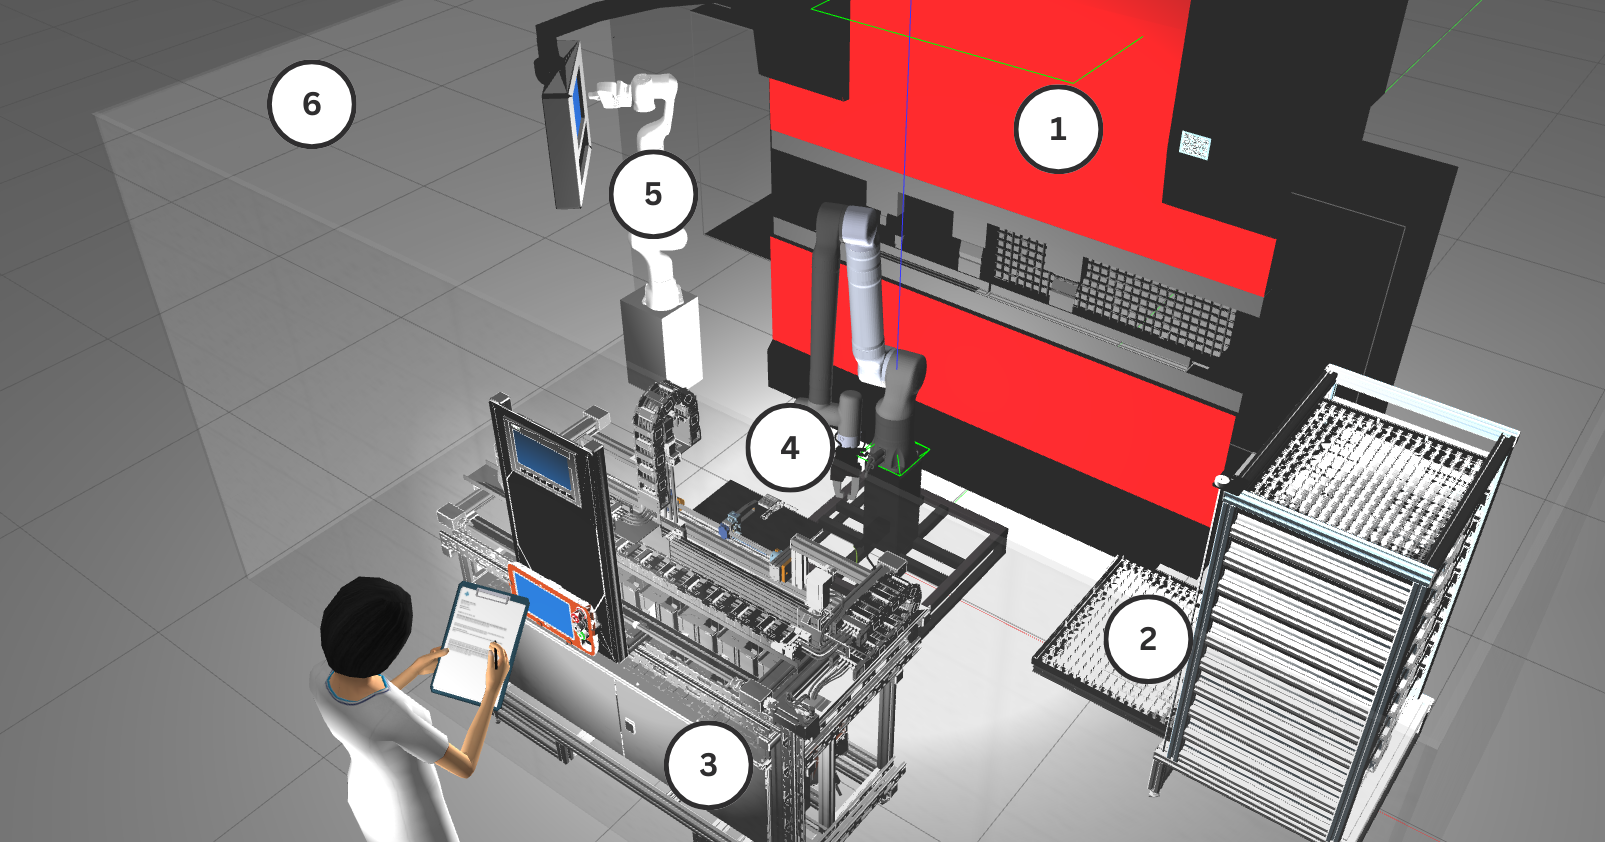
\includegraphics[width=\textwidth]{figures/robotic-workcell1.png}
    \caption{Robotic workcell layout. 1) Bending machine 2) Storage station 3) Unloading station 4) Handling robot 5) Bending machine terminal operating robot 6) Safety fence}
    \label{fig:robotic-workcell}

\end{figure}

% Create a figure of robotic workcell flow of things
\begin{figure}[h]
    \centering
    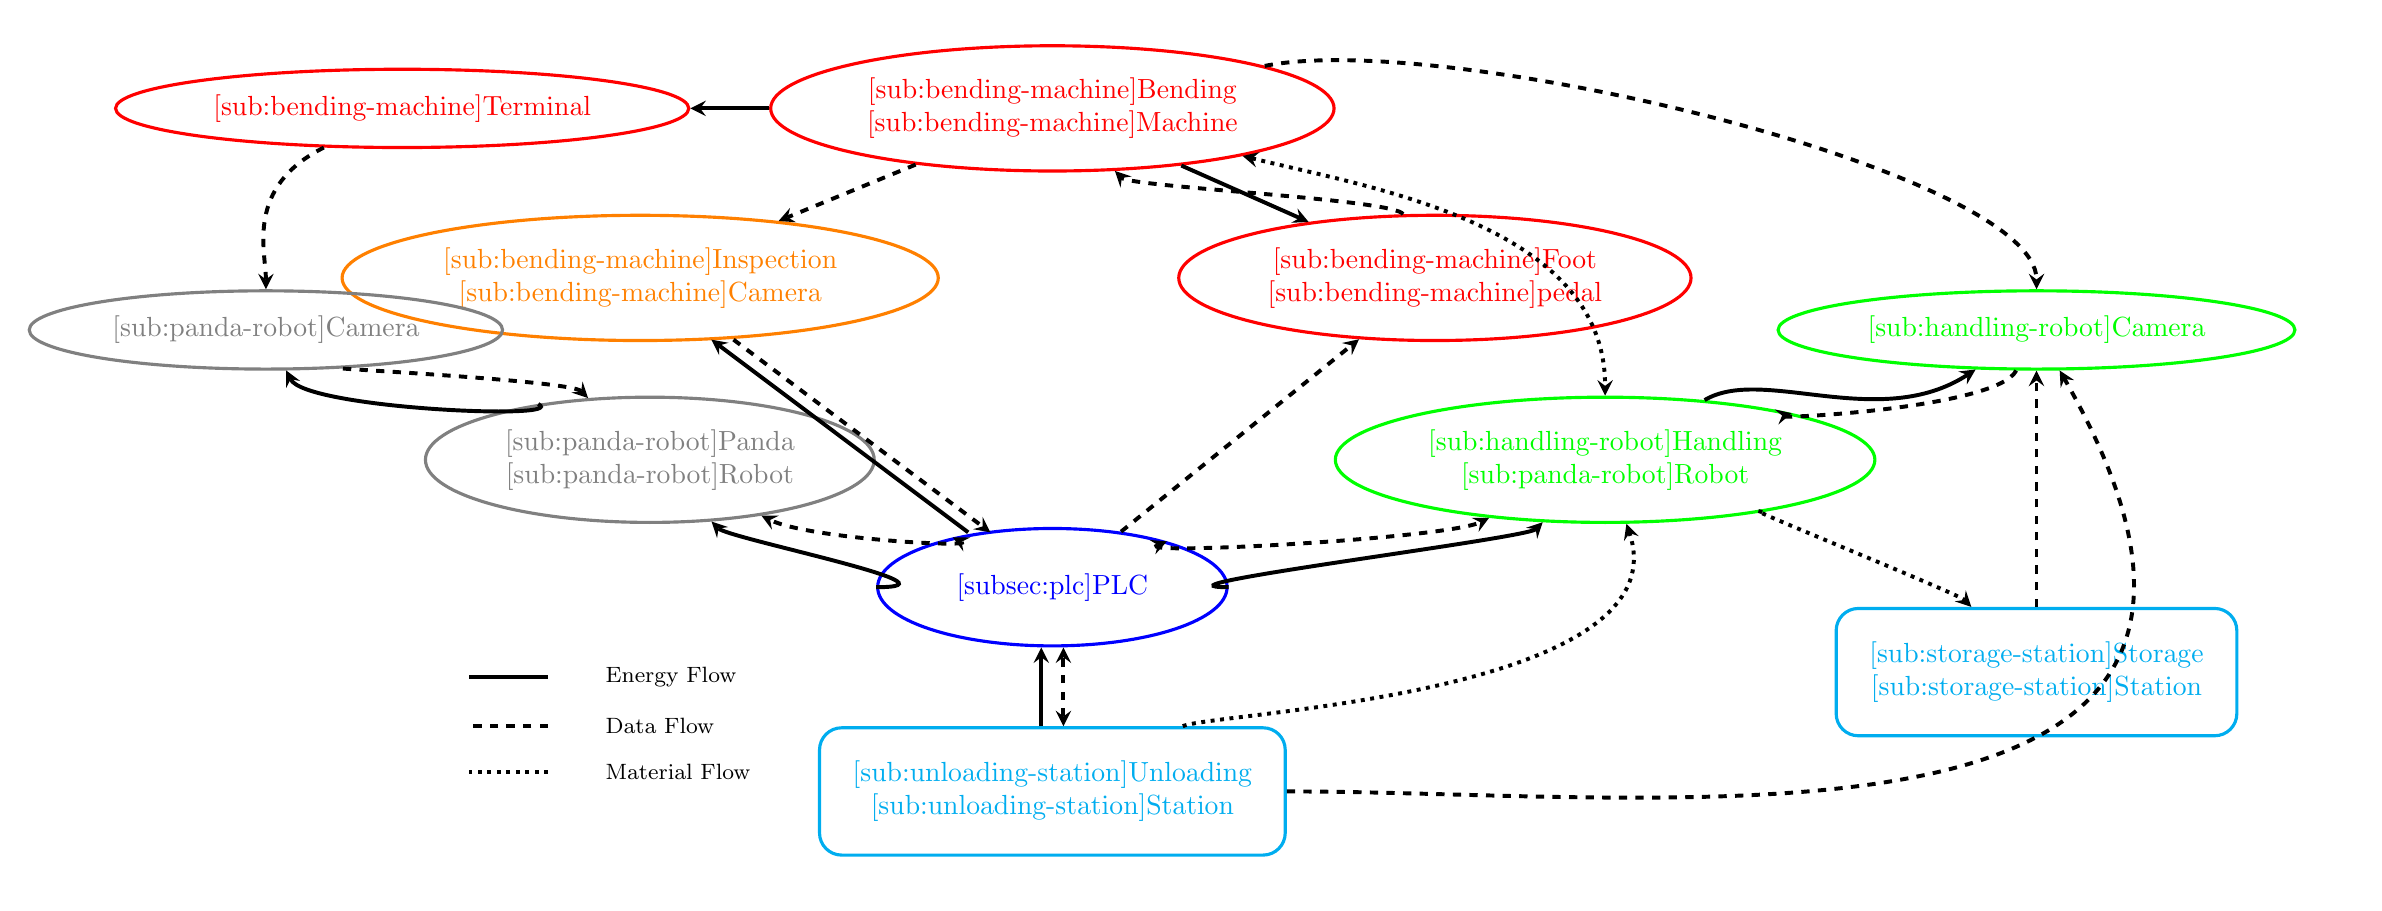
\begin{tikzpicture}[
        every node/.style={draw, ellipse, align=center, inner sep=5pt, line width=0.4mm},
        rect/.style={draw=cyan, rectangle, rounded corners=8pt, align=center, inner sep=12pt},
        energy/.style={->, >=stealth, thick, line width=0.5mm},
        data/.style={->, >=stealth, dashed, line width=0.5mm},
        material/.style={->, >=stealth, dotted, line width=0.5mm},
        node distance=1cm
    ]
      
        % Nodes
        \node (bending) [red] {\hyperref[sub:bending-machine]{Bending}\\ \hyperref[sub:bending-machine]{Machine}};
        \node (terminal) [red, left=of bending] {\hyperref[sub:bending-machine]{Terminal}};
        \node (camera1) [orange, below left=1cm and 0cm of bending] {\hyperref[sub:bending-machine]{Inspection}\\ \hyperref[sub:bending-machine]{Camera}};
        \node (footpedal) [red, below right=1cm and 0cm of bending] {\hyperref[sub:bending-machine]{Foot}\\ \hyperref[sub:bending-machine]{pedal}};
        \node (plc) [blue, below=4.5cm of bending, inner sep=10pt] {\hyperref[subsec:plc]{PLC}};
        \node (pandarobot) [gray, above left=0.5cm and 1.5cm of plc] {\hyperref[sub:panda-robot]{Panda}\\ \hyperref[sub:panda-robot]{Robot}};
        \node (handlingrobot) [green, above right=0.5cm and 3cm of plc] {\hyperref[sub:handling-robot]{Handling}\\ \hyperref[sub:panda-robot]{Robot}};
        \node (camera3) [green, above right=of handlingrobot] {\hyperref[sub:handling-robot]{Camera}};
        \node (storage) [rect, below=3cm of camera3, text=cyan] {\hyperref[sub:storage-station]{Storage}\\ \hyperref[sub:storage-station]{Station}};
        \node (camera2) [gray, above left=of pandarobot] {\hyperref[sub:panda-robot]{Camera}};
        \node (unloading) [rect, below=of plc, draw=cyan, text=cyan] {\hyperref[sub:unloading-station]{Unloading}\\ \hyperref[sub:unloading-station]{Station}};
        \node (energy) [rectangle, draw=none, fill=white, text width=2.5cm, align=left, above left=0.3cm and 0cm of unloading, font=\footnotesize] {Energy Flow};
        \node (data) [rectangle, draw=none, fill=white, text width=2.5cm, align=left, below=0cm of energy, font=\footnotesize] {Data Flow};
        \node (material) [rectangle, draw=none, fill=white, text width=2.5cm, align=left, below=0cm of data, font=\footnotesize] {Material Flow};
        \node (energy_left) [circle, draw=none, left=0cm of energy] {};
        \node (energy_right) [circle, draw=none, left=1cm of energy_left] {};
        \node (data_left) [circle, draw=none, left=0cm of data] {};
        \node (data_right) [circle, draw=none, left=1cm of data_left] {};
        \node (material_left) [circle, draw=none, left=0cm of material] {};
        \node (material_right) [circle, draw=none, left=1cm of material_left] {};
        
        % Energy flow
        \draw[energy] (bending) -- (terminal);
        \draw[energy] (bending) -- (footpedal);
        \draw[energy, transform canvas={xshift=-4pt}] (plc) -- (camera1);
        \draw[energy] (plc) .. controls ++(-1, 0) and ++(1,-1) .. (pandarobot);
        \draw[energy] (pandarobot) .. controls ++(-1, 0.5) and ++(0.5,-1) .. (camera2);
        \draw[energy] (plc) .. controls ++(1, 0) and ++(-1,-1) .. (handlingrobot);
        \draw[energy] (handlingrobot) .. controls ++(2,1.2) and ++(-2,-1.3) .. (camera3);
        \draw[energy, transform canvas={xshift=-4pt}] (unloading) -- (plc);
        
        % Data flow
        \draw[data] (terminal) .. controls ++(-2,-1) and ++(0,1) .. (camera2);
        \draw[data] (camera2) .. controls ++(1, -0.5) and ++(-1,1) .. (pandarobot);
        \draw[data] (camera3) .. controls ++(-0.5,-1) and ++(2,0.5) .. (handlingrobot);
        \draw[data] (bending) -- (camera1);
        \draw[data] (plc) -- (footpedal);
        \draw[data] (storage) -- (camera3);
        \draw[data] (bending) .. controls ++(5,1) and ++(0,2) .. (camera3);
        \draw[data, transform canvas={xshift=4pt}] (camera1) -- (plc);
        \draw[data, <->, transform canvas={xshift=4pt}] (unloading) -- (plc);
        \draw[data, <->] (plc) .. controls ++(-1, 0.5) and ++(2,-1) .. (pandarobot);
        \draw[data, <->] (plc) .. controls ++(1, 0.4) and ++(-2,-1) .. (handlingrobot);
        \draw[data] (unloading) .. controls ++(8,0) and ++(4,-7) .. (camera3);
        \draw[data] (footpedal) .. controls ++(-0.5,1) and ++(1,-1) .. (bending);

        % Material flow
        \draw[material] (unloading) .. controls ++(2,1) and ++(1,-3) .. (handlingrobot);
        \draw[material] (handlingrobot) .. controls ++(1.5,-0.5) and ++(-1,1) .. (storage);
        \draw[material, <->] (bending) .. controls ++(4,-1) and ++(0,3) .. (handlingrobot);

        % Create legend for the figure
        \draw[energy,-] (energy_left) -- (energy_right);
        \draw[data,-] (data_left) -- (data_right);
        \draw[material,-] (material_left) -- (material_right);

    \end{tikzpicture}
    \caption{Energy, data and material flow in the robotic workcell}
    \label{fig:flow-workcell}
\end{figure}



\subsection{Bending machine}
\label{sub:bending-machine}

\subsection{Storage station}
\label{sub:storage-station}

\subsection{Unloading station}
\label{sub:unloading-station}

\subsection{Handling robot}
\label{sub:handling-robot}

\subsection{Bending machine terminal operating robot}
\label{sub:panda-robot}

\subsection{Safety fence}
\label{sub:safety-fence}






\section{Requirements for the overall system}
\begin{enumerate}
    \item A key requirement for the mobile robot unit is to be able to cope with the limited space available in the
    project partner's production hall. Specifically, this means that only an area of approximately $2 m \times 4.5 m$ is
    available in front of the sheet metal bending machine.

    \item Another point is the operating time of the overall system. The unit should be able to autonomously
    manage a day shift of eight hours and a night shift of six hours without any major personnel
    intervention.

    \item Robot should also be able to handle various sheet metal part variants, i.e. different component sizes and
    geometries. In addition to the flexible handling of different sheet metal parts, the focus is also on the
    simple integration of new variants into the existing system. Some of the sheet metal parts in production are
    of small size. These sheets will have little gripping surface after few bendings. Special considerations needs to be given to the
    gripper design so that robot can handle sheet metal parts of small and medium sizes. (from $60 mm \times 110 mm$ to upto $115 mm \times 220 mm$)
    The sheets should not move in the gripper during the movement of the robotic arm.

    \item 
    The mobile robot unit is to be used as a supplement to manual production. It is therefore necessary
    that it can be set up and dismantled quickly and easily in front of the bending machine.

    \item The hand-eye calibration using a vision sensor could degrade over time due to environmental factors such as temperature changes or vibrations. \cite{Bahadir2024}
    This will decrease the accuracy of robot \hyperref[acro:TCP]{TCP} in positioning and grasping leading to incorrect bending.
    The robot should be able to automatically recalibrate without any long delays when there is a request by the operator.
    
    \item The angle measurement on the bent sheet should be carried out using a camera system
    after each bending process. Based on the measured angle, bending machine should be re-adjusted for the next iteration. The
    necessary values should also be entered at the operator terminal by the terminal operating robot. In addition, a
    continuous real-time status query of the bending machine is required via the operating terminal. For
    the implementation of this subtask, the company is working with \textbf{VisCheck GmbH}, which specializes in
    reading screens using a camera and making entries via a robot.
    
\end{enumerate}








\section{Hardware Selection}
\subsection{AMADA bending machine}
% Table for bending machine details
\begin{table}[h!]
    \centering
    \renewcommand{\arraystretch}{1.2} % Adjusts row height
    \small
    \begin{tabular}{ll}
        {\textbf{Description}} & {\textbf{Value}} \\
        \hline
        \textbf{Model} & HFP 50-20 \\
        \textbf{Manufacturer} & \hyperref[acro:AMADA]{AMADA} (France) \\
        \textbf{Year of manufacture} & 2005 \\
        \textbf{Drive} & Hydraulic press brake \\
        \textbf{Pressing capacity} & 500 kN \\
        \textbf{Working length} & 2090 mm \\
        \textbf{Distance between frames} & 1665 mm \\
        \textbf{\hyperref[acro:CNC]{CNC} control} & AMADA AMNC \hyperref[acro:3D]{3D}-graphic \\
        & with \hyperref[acro:TFT]{TFT} color screen \\
        \textbf{controlled axes} &  Y1/Y2; X1/X2; R1/R2; Z1/Z2 \\
        \textbf{Open height} & 470 mm \\
        \textbf{Stroke} & 200 mm \\
        \textbf{Bending Speed} & 10 mm/s \\
        \textbf{Approach Speed} & 100 mm/s \\
        \textbf{Return Speed} & 100 mm/s \\
        \textbf{Laser monitoring} & FIESSLER \\
        \textbf{Length x width x height} & 3458 mm x 2450 mm x 2450 mm \\
        \textbf{Weight} & 4850 kg \\ \hline
    \end{tabular}
    \caption{Bending Machine Technical Specifications (Source: \cite{bmspecifications})}
    \label{tab:machine_specifications}
\end{table}



\subsection{Kassow Robots: KR1410}

KR1410 is a 7-axis collaborative robotic arm from Kassow Robots. It has a reachability of 1400 mm which fits
satisfactory in the workcell. A seventh axis is particulary useful as it allows more freedom during trajectory planning
especially in close spaces.

The robotic arm comes with a robot controller and a teach pendant as shown in Figure \ref{fig:kassow-robot-parts} A robot controller is the main controlling unit for each \hyperref[acro:KR]{KR} manipulator.
Teach Pendant is used for programming the manipulator and also provides \hyperref[acro:UI]{UI} and safety controls.
KR1410 could be interfaced with ROS. KR provides packages to install through which KR messages transmission is set up.

\begin{figure}[h]
    \centering
    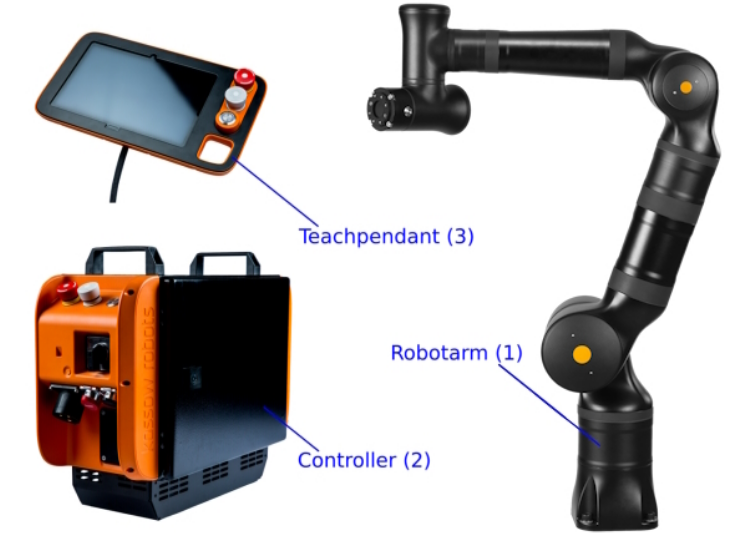
\includegraphics[width=0.5\textwidth]{figures/kassow-robot-parts.png}
    \caption{Functional parts of the KR collaborative robot (Source: \cite{kassow-manual})}
    \label{fig:kassow-robot-parts}
\end{figure}

\subsubsection{Function Description}
Function Description
\begin{enumerate}
    \item 
\end{enumerate}
The industrial robot arm is a robot system used for manufacturing. It is automated, programmable and
capable of moving within up to seven axes.
The robot is typically used for welding, painting, assembly, pick and place, packaging and labelling.
\begin{table}[h!]
    \centering
    \small
    \renewcommand{\arraystretch}{1.2} % Adjusts row height
    \begin{tabular}{ll}
        \textbf{Description} & \textbf{Value} \\ \hline
        Type & Collaborative \\
        Reach & 1400 mm in all directions\\
        Number of axis & 7-axis \\
        Operating temperature range & 0-45°C\\ 
        Weight & 38.0 kg \\ 
        AC Power connector & 1 Phase CEE \\ 
        Typical Power consumption & 400-1200W \\ 
        Supply voltage & 100-120 and 200-240 VAC (50/60hz) \\ 
        Supply current & 16A\\ 
        \hyperref[acro:IO]{IO} power supply & 24 VDC\\ 
        Max. joint speed  & 163/225 °/s\\ 
        Max. static force on \hyperref[acro:TFC]{TFC} (payload) & 10 kg\\ 
        Max. static torque on \hyperref[acro:TFC]{TFC} & 25 Nm\\ 
        Sound level & Below 70dB (A) \\ 
        Ingress protection & IP54 \\ 
        Joint ranges & Joint 1,3,5,6,7 +/- 360° \\
        & Joint 2,4 -70/+180° \\ 
        Footprint& $160 \times 160$ mm \\ 
        ROS Support & Available \\ \hline
    \end{tabular}
    \caption{KR1410 Technical Specifications (Source: \cite[page 31]{kassow-specification})}
    \end{table}

    \subsubsection{Increased Safety}

    Industrial Robotic Automation significantly enhances workplace safety. Robots, especially cobots like Kassow Robot's 7-axis version, are equipped with advanced safety features and mechanisms. 
    They can detect and avoid collisions with people or objects, reducing the risks associated with manual labour in potentially hazardous environments. This commitment to safety exemplifies the primary objective of robotic automation: to protect workers and streamline processes.

    \subsubsection{More Flexibility}
    Cobots, with their adaptable designs, represent the epitome of flexibility in industrial automation. 
    Unlike traditional fixed robots, the 7-axis from Kassow Robots can be quickly reprogrammed and adapted for different tasks. This agility makes them an invaluable asset for industries undergoing frequent changes or those with diverse product lines.

    \subsubsection{Cost-effective}
    Introducing Industrial Robotic Automation is a wise financial decision for businesses. Cobots, which offer a competitive price point compared to traditional industrial robots, provide significant returns on investment by improving efficiency, reducing waste, and minimizing production downtime. 
    The long-term savings, in terms of both time and money, underscore the economic benefits of integrating robotic automation into the production process.

    \subsubsection{Great Scalability}
    Industrial robots, especially cobots, are inherently scalable. Whether it's adjusting to a new product line or ramping up production volumes, Kassow Robot's 7-axis cobot can be swiftly recalibrated to meet evolving demands. 
    This ensures that industries can easily scale their operations without undergoing extensive overhauls or incurring excessive costs.

    \subsubsection*{Improved Quality}
    Quality assurance is a prominent benefit of Industrial Robotic Automation. Robots, with their precision and consistency, dramatically reduce the margin for errors in production. 
    Kassow Robot's 7-axis model ensures that each task—from welding to assembly—is executed with remarkable accuracy, leading to products of superior quality and consistency.

    \subsubsection*{Higher Productivity}

    Robotic automation directly translates to increased productivity. By automating repetitive and time-consuming tasks, cobots free human workers to concentrate on value-added activities. 
    In scenarios where cobots collaborate with human workers, the synergy often leads to faster production cycles, efficient workflows, and overall heightened productivity.

    
\subsection{VISOR\textsuperscript{\textregistered} Vision Sensor}
\label{sec:visor}
    According to \hyperref[acro:VISOR]{VISOR}\textsuperscript{\textregistered} \cite[page 22]{visor_user_manual} user manual, the \hyperref[acro:VISOR]{VISOR}\textsuperscript{\textregistered} vision sensor is an optical sensor and is used for the non-contact acquisition or identification of objects.
    The vision sensor features a number of different evaluation methods (detectors), with the specific methods
    depending on the specific model sensor. The product is designed for industrial use only. The \hyperref[acro:VISOR]{VISOR}\textsuperscript{\textregistered} vision sensor is a cost-effective alternative to conventional image processing systems.

    \hyperref[acro:VISOR]{VISOR}\textsuperscript{\textregistered} vision sensor is a suitable choice for the identification and classification of metal sheets for the automated bending process.
    These sensors enable precise detection and processing of features on sheets, which leads to the efficiency and accuracy of automated bending process.
    Special considerations need to be taken in complex industrial environments, where light reflections or changing extraneous light can distort evaluation results. For this reason, an external light source is used to protect against ambient light.

    \subsection{Robotic Camera}
    \label{subsec:robotic-camera}

    \subsection{Inspection Camera}
    \label{subsec:inspection-camera}

\section{Software Architecture}
To find out the software version and development environment used in the development of the workcell, check the appendix \ref{sec:versions}.


\subsection{Simulation Software}
\label{subsec:simulation-software}
Before building the robotic workcell in the real world, the kassow robot is simulated in the ROS and gazebo environment.

\subsubsection{ROS}
\label{subsubsec:ROS}
For more information on ROS, see section \ref{subsec:ROS}. First, a URDF model of the KR1410 with gripper attached is created
complete with all positions of links, joints, sensors, models etc. This URDF description of robot is then ready to be tested
in the workcell.

The robotic motion of unloading station gripper and the manipulation of KR1410 using the robotic gripper is simulated using ROS. (See Figure \ref{fig:gazebo-rviz})

\begin{figure}[h]
    \centering
    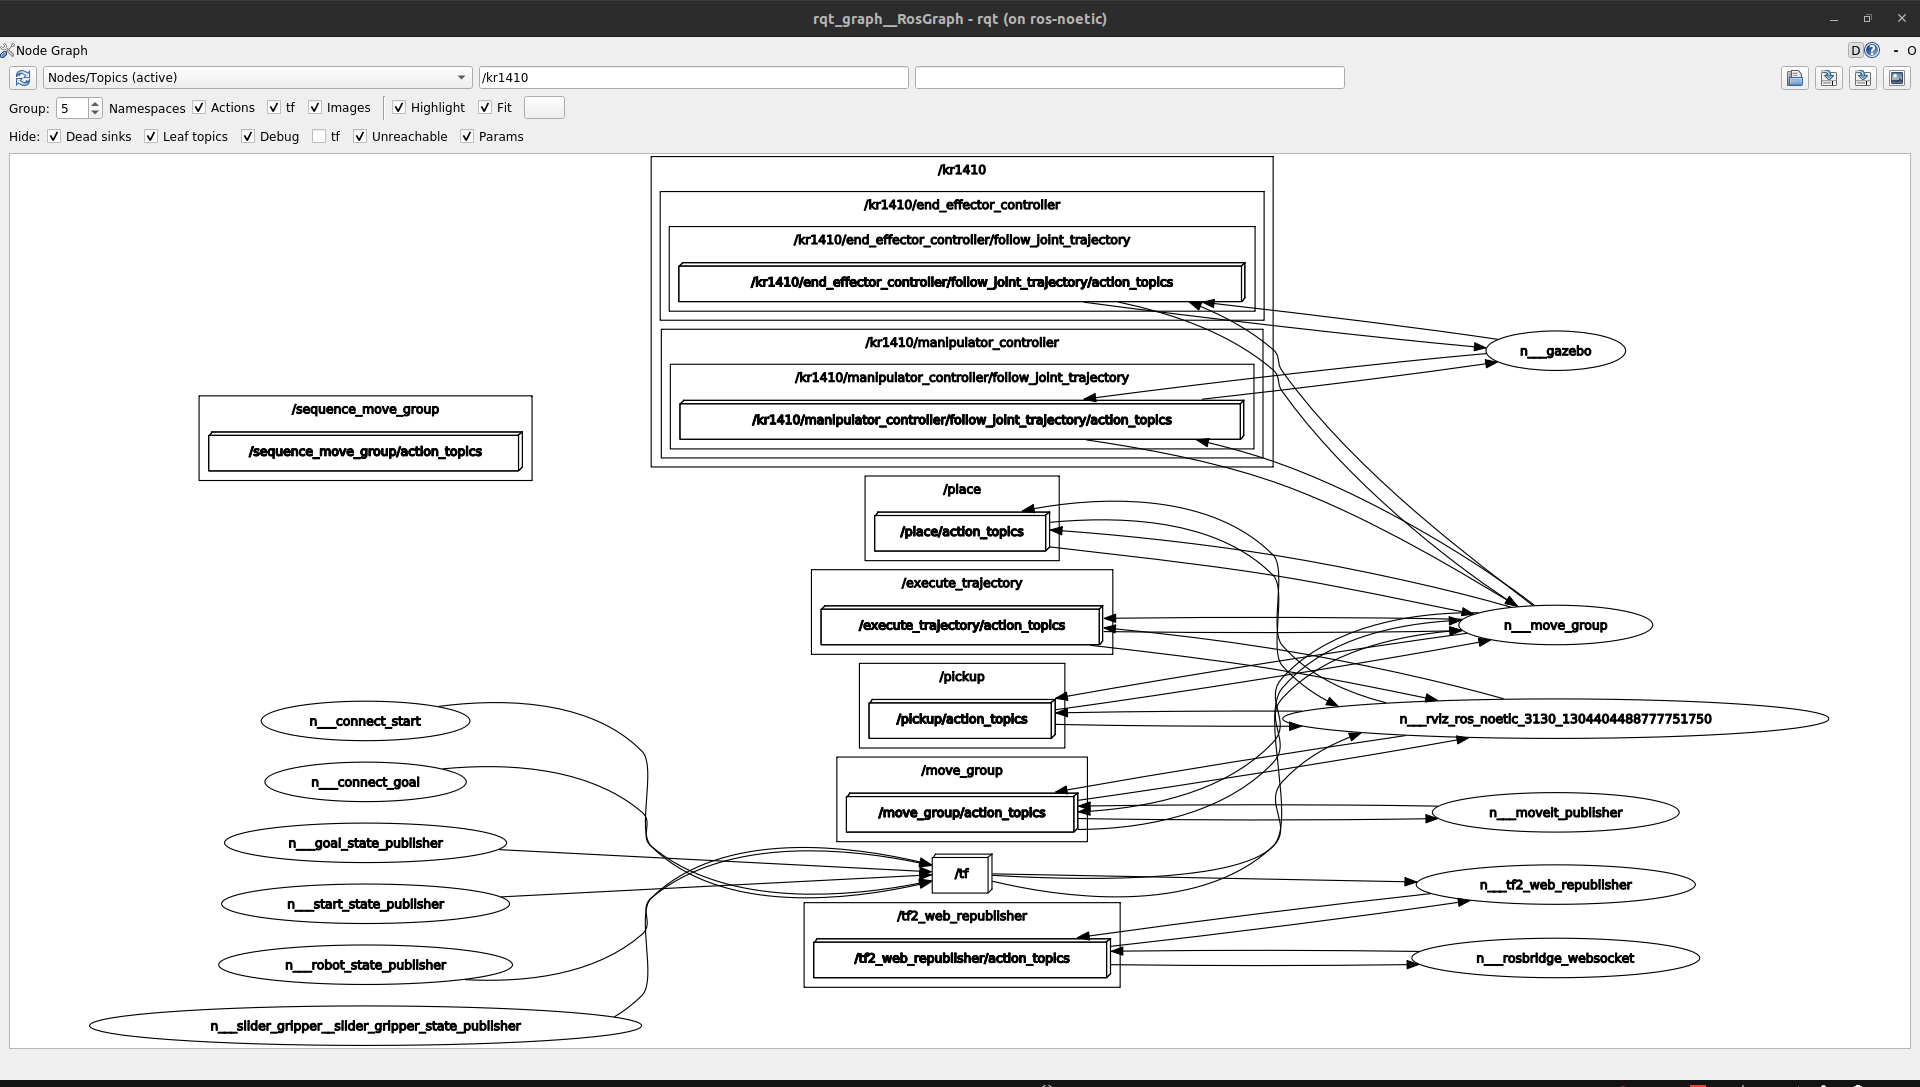
\includegraphics[width=\textwidth]{figures/rosgraph.png}
    \caption{ROSGraph}
    \label{fig:rosgraph}
\end{figure}

Many custom ROS packages \cite{rospackage} are created to simulate the workcell. A single ROS launch \cite{roslaunch} file is launched to run every node \cite{rosnode}, service \cite{rosservice} and parameter \cite{parameterserver} or action servers \cite{actionserver}
Figure \ref{fig:rosgraph} visualizes the computation graph of the simulation. It shows the currently active ROS nodes \cite{rosnode}
and topics \cite{rostopic} in the simulation of robotic workcell.



\subsubsection{Gazebo Simulator}
\label{subsubsec:gazebo}
Gazebo is a 3D dynamic simulator with the ability to accurately and efficiently simulate populations
of robots in complex indoor and outdoor environments. While similar to game engines, Gazebo
offers physics simulation at a much higher degree of fidelity, a suite of sensors, and interfaces for
both users and programs. \cite{gazebo-classic}

A model of the entire workcell is created for the gazebo simulator. The assets are converted from CAD designs
to .dae and .stl file format using blender software. These meshes are then included in the SDF model object.
The workcell is then ready to be simulated in the gazebo simulator.

\begin{figure}[h]
    \centering
    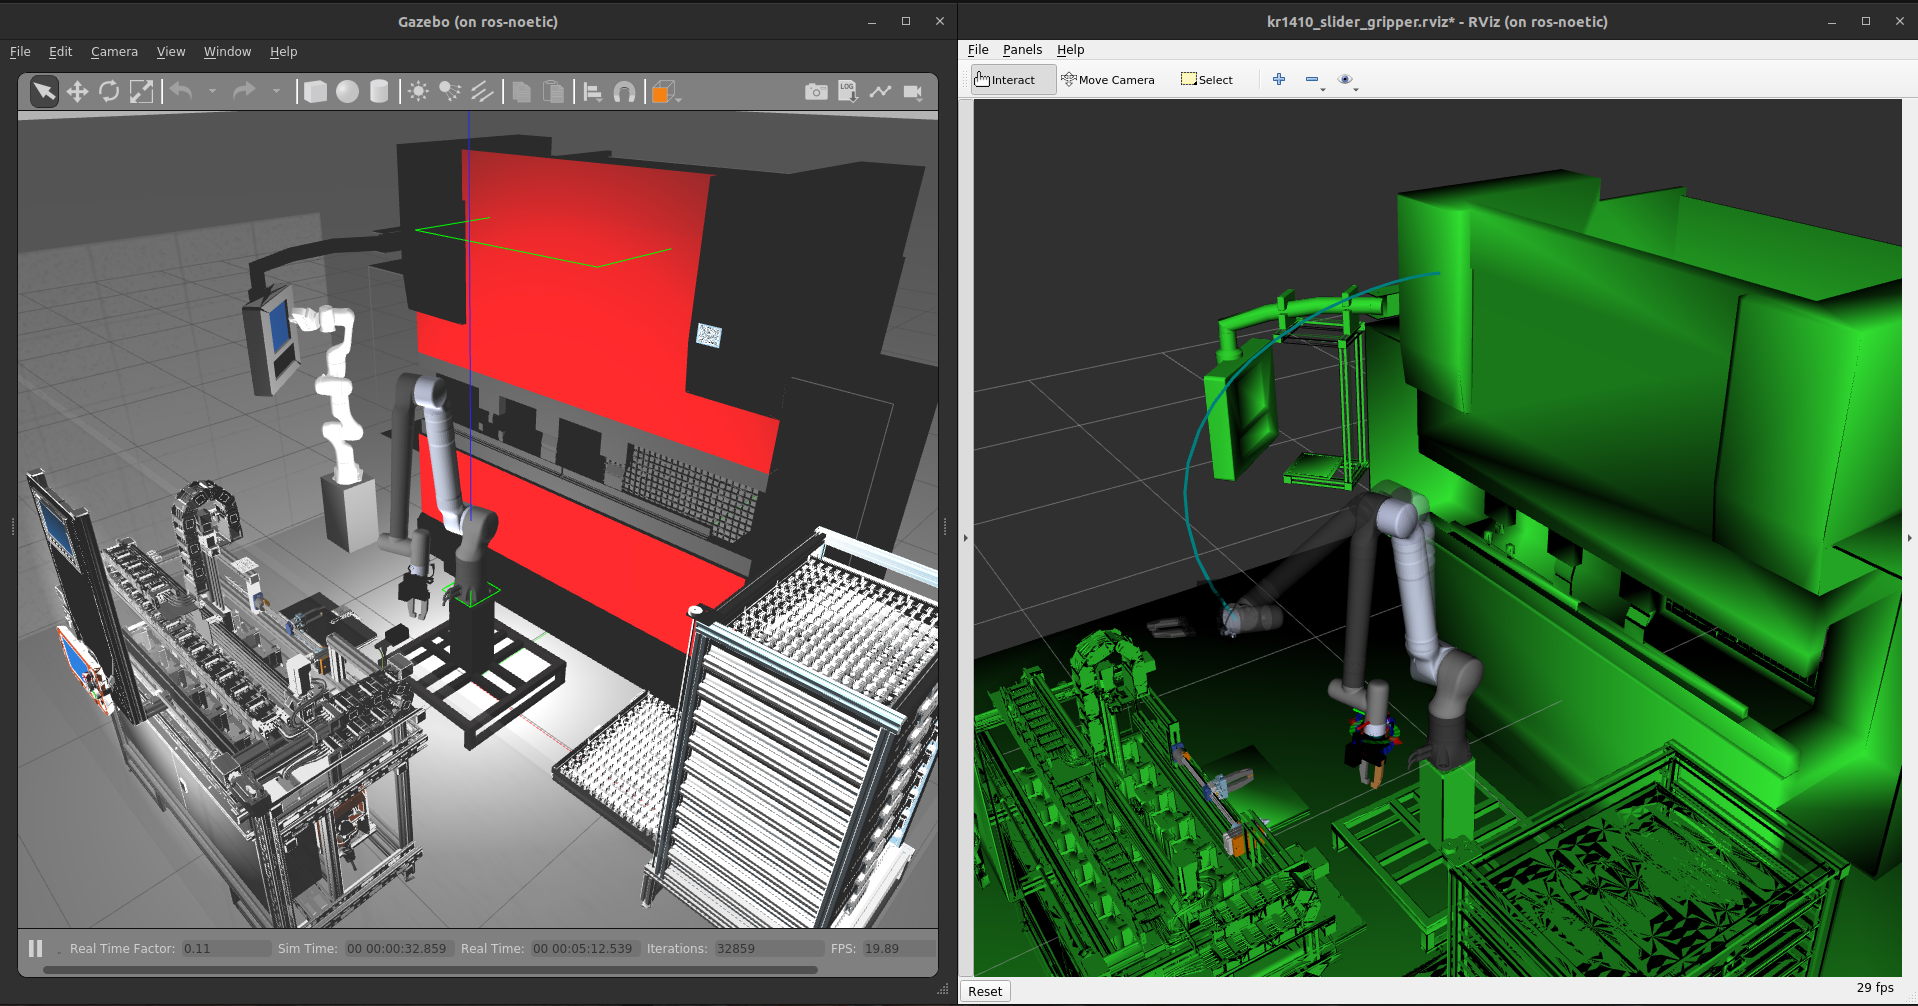
\includegraphics[width=\textwidth]{figures/gazebo-rviz.png}
    \caption{Robotic workcell in Gazebo simulator (left) and RViz (right)}
    \label{fig:gazebo-rviz}
\end{figure}

\subsubsection{RViz}
\label{subsubsec:RViz}
RViz is short for ROS Visualization. It is a 3D visualization software tool for robots, sensors, and algorithms.
It allows seeing the robot's perception of its world (real or simulated).
The purpose of rviz is to enable you to visualize the state of a robot. It uses sensor data to try
to create an accurate depiction of what is going on in the robot's environment.

In

\subsubsection{MoveIt}
\label{subsubsec:moveit}


\subsection{\hyperref[acro:VISOR]{VISOR}\textsuperscript{\textregistered} Communication Setup}
\label{subsec:computer-vision}
VISOR software is not officially supported by the KR1410 and there is no direct integration of the VISOR camera available.
However, Kassow robots provides support to build own software through CBun development.
The CBun (Capability Bundle) represents a modular framework within the KR software system,
which encapsulates functionalities and provides the
access to its predefined \hyperref[acro:API]{API}.


\begin{figure}[h]
    \centering
    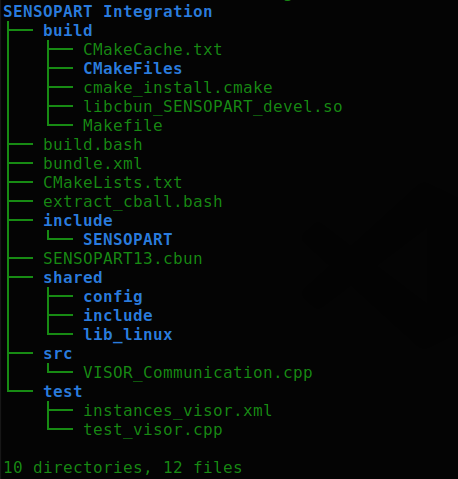
\includegraphics[width=0.5\textwidth]{figures/sensopart-development.png}
    \caption{CBun Project Setup for SENSOPART Integration in KR}
    \label{fig:sensopart-development}
\end{figure}


The CBun SDK is the Software Development Kit that provides all essential tools
for CBun development. The project setup is created in a Visual Studio Code container
running on Ubuntu 18.04 with a special set of software packages. \cite{Cbun}
The header files are located in \textbf{include} directory and C++ source file \textit{i.e.}     \textit{VISOR\_Communication.cpp}
are placed in \textbf{src} directory.
Upon building the project, a \textit{SENSOPART.cbun} file is generated as shown in \ref{fig:sensopart-development}
It is then installed in the teach pendant using a \hyperref[acro:USB]{USB}. Figure \ref{fig:cbun-variables}
shows the information of VISOR variables getting through the VISOR to KR1410.

\begin{figure}[h]
    \centering
    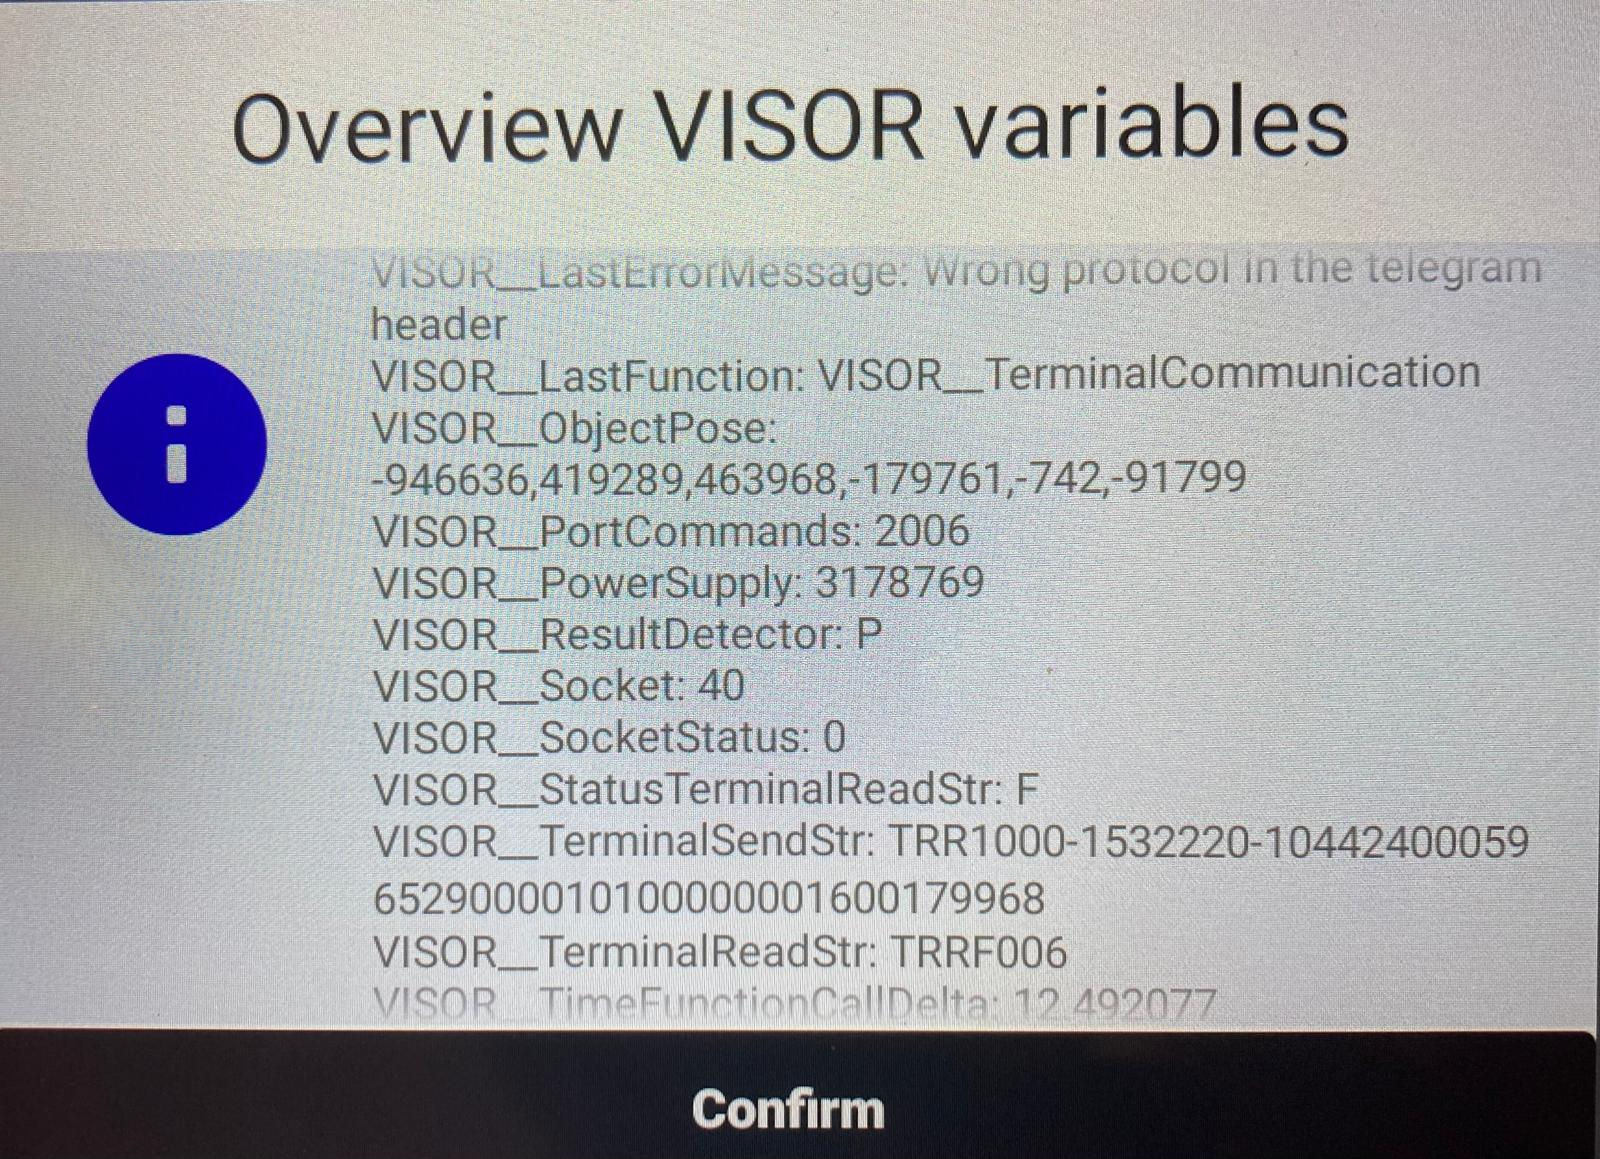
\includegraphics[width=0.55\textwidth]{figures/visor-cbun-connection.png}
    \caption{Dialog Box showing current VISOR variables}
    \label{fig:cbun-variables}
\end{figure}

CBun device is one of the CBun elements. CBun Device concept allows to wrap handling code of physical device like VISOR vision sensor into the CBun and hide it from the end user. This allows the user to simply control and monitor devices without the need to implement the communication and logic. \cite{cbun-device}

VISOR camera is powered from the TPSU02 on the KR1410 tool-IO.
A CBun device named \textbf{VISOR} from CBun developement is created which has methods for
controlling the functionalities of camera like changing job, getting object pose by triggering camera and performing calibration. Through this
device, the KR communicates with the VISOR over telegram.



\subsection{Program Tree}
\label{subsec:program-tree}
Kassow Robots teach pendant is a graphical user interface which allows users
to control robot arm and \hyperref[acro:HW]{HW} equipment, build and run programs and configure robot installation setup.
It is intended to be intuitive as it comes with familiar design of a tablet. The main screen interface is based
on a double pane layout between which there is a command box. The command box provides access to basic building blocks,
loaded CBun devices, and subroutines defined by the operator. These commands can be dragged and dropped into the program
tree. \cite[page 15]{kassow-software-manual}
There is a control mode in the bottom which can set the master speed or launch the program and control the execution process. (pause, continue, terminate). The program tree view is where the robot program is built in an intuitive graphical way.
A program tree contains at least one sequence. A sequence contains a number of commands that are executed sequentially.
For separate sequences, the commands are executed simultaneously and asynchronously. \cite[page 20]{kassow-software-manual}


\begin{figure}[h]
    \centering
    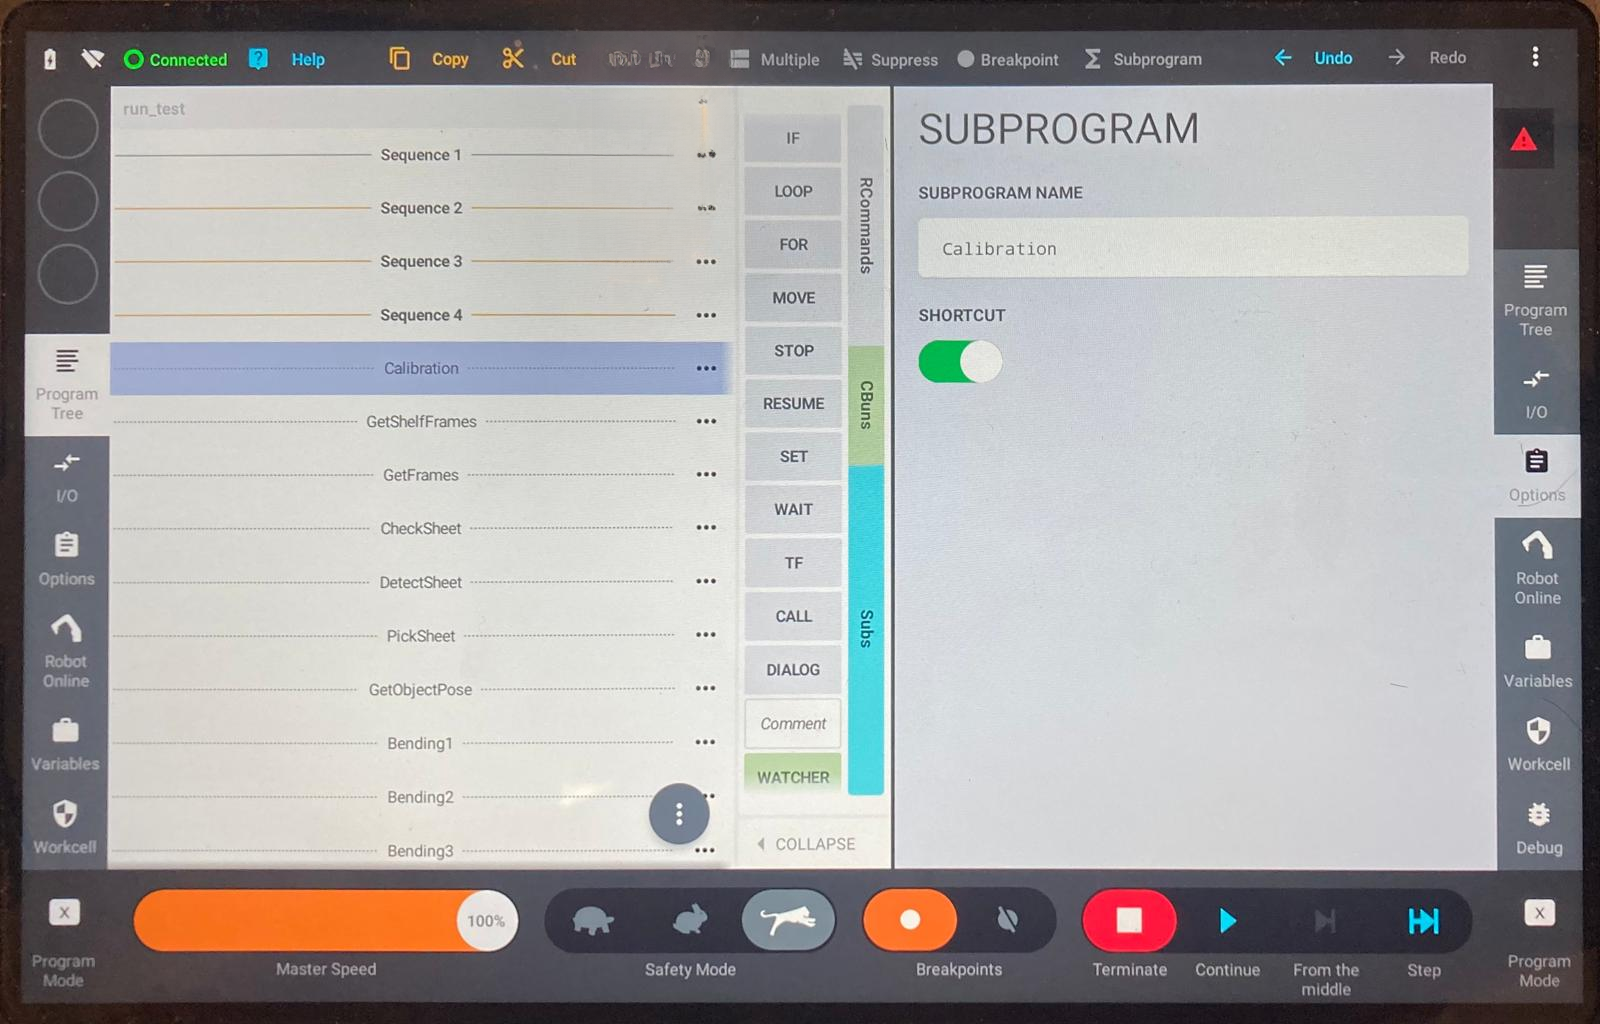
\includegraphics[width=\textwidth]{figures/programtree.png}
    \caption{Programming in teach pendant for a sheet metal part variant}
    \label{fig:programtree}
\end{figure}


The programming of \hyperref[acro:KR]{KR1410} is done in the program tree for one sheet metal part variant.
It is done to test the bending process using the \hyperref[acro:KR]{KR1410}.
The program tree of the workcell consists of four sequences which runs in parallel.
Sequence 1 is the main program which runs all the pick-place and bending operations.
Sequence 2 and 3 looks for a signal from \hyperref[acro:PLC]{PLC} for pausing and terminating the current program
respectively. Sequence 4 controls the robotic and unloading station grippers using a push button
for manual operation of the gripper in case of emergency.

The robot is programmed using a number of subprograms such that a subprogram
can be quickly imported in the sequence and is intuitive to understand as shown in figure \ref{fig:programtree}
Besides normal RCommands like IF, LOOP, FOR, MOVE, WAIT and so on, there are a number of CBun devices
from Kassow Robots
imported like the IK, FK and WATCHER devices. IK is used to get the inverse
kinematics from a pose and FK is used to get the forward kinematics
from a joint configuration.
Custom made CBuns modules for \hyperref[acro:VISOR]{VISOR}\textsuperscript{\textregistered}
are also used for auto-calibration and for getting the pose in the
robot frame of a detected object in the workspace using the \hyperref[acro:VISOR]{VISOR}\textsuperscript{\textregistered} vision sensor.



\subsection{Web UI}
\label{subsec:web-ui}

\subsubsection{Front-end technologies}
\label{subsubsec:frontend}
Front-end development is the development of visual and interactive elements of a website that users interact with directly. It's a combination
of HTML, CSS and JavaScript, where HTML provides the structure, CSS the styling and layout, and JavaScript the dynamic behaviour and interactivity.
\cite{frontend}

\paragraph{Reactjs}
\label{par:reactjs}
is the most popular front-end JavaScript library for building user interfaces. React can also render on the server using Node and power mobile
apps using React Native. It user interfaces out of individual pieces called components written in JavaScript.
\cite{reactjs}

\subsubsection{Backend technologies}
\label{subsubsec:backend}

Backend development refers to the server-side aspect of web development, focusing on creating and managing the server logic, databases,
and APIs. It involves handling user authentication, authorization, and processing user requests, typically using backend development
languages such as Python, Java, JavaScript (Node.js), and .NET. \cite{backend}

\paragraph{Node.js}
\label{par:nodejs}
is an open-source, cross-platform JavaScript runtime environment that lets developers create servers, web application etc.
The web application for robotic workcell is built and hosted on a Node.js server. \cite{nodejs}

\paragraph{npm}
\label{par:npm}
is a package manager for Node.js. It stands for Node Package Manager. Through this, ROS web tools for server-side runtime are installed like
roslib, ros3djs. \cite{npm}

\subsubsection{ROS Web Tools}
\label{subsubsec:rosweb}

Robot Web Tools are open-source libraries and tools for building web-based robot apps with ROS. Rosbridge, roslibjs, ros3Djs, and visualization-rwt packages
are used for building the web application which are part of ROS Web Tools. \cite{webtools} Rosbridge and visualization-rwt are installed on the ROS workspace
for robotic workcell. Roslibjs and ros3Djs are libraries for building the web application and are installed on the server built on Node.js.

\paragraph{Rosbridge}
\label{par:rosbridge}
The WebSocket makes it possible to open a two-way interactive communication session between the user's browser and a server.
With this API, messages can be sent to a server and received through event-driven responses without having to poll the server for a reply. \cite{websocket}
Rosbridge provides a websocket interface to ROS systems. It will provide interface to front-end technologies like ReactJs which builds the UI
and publishes a web application. Rosbridge suite is a meta-package containing rosbridge, various front end packages for Rosbridge 
like a WebSocket package, and helper packages. \cite{rosbridge}

\paragraph{roslibjs}
\label{par:roslibjs}
provides base dependencies and support libraries for ROS. roslib contains many of the common data structures and tools that are shared across
ROS client library implementations. \cite{roslib} It will provides support to interact with basic ROS functionalities like topics, services, parameter servers and others.

\paragraph{ros3djs}
\label{par:ros3djs}
is the standard JavaScript 3D visualization manager for ROS. It is build ontop of roslibjs and utilizes the power of three.js \cite{threejs}.
Many standard ROS features like interactive markers, URDFs, and maps are included as part of this library. \cite{ros3djs}

\paragraph{visualization-rwt}
\label{par:visualization-rwt}
package is a suite of nodes for web based robot visualization. It provides nodes for controlling the robot using MoveIt through web application.
\cite{visualization-rwt}





\section*{Chapter 4: Hardware Integration}

\chapter{Software Development}

\setcounter{section}{0}
\setcounter{subsection}{0}

\section{Control Software}

\section{Camera 1: Feature Detection}

\section{Camera 2: Inspection and Quality Control}

\section{Web Interface Design}



\chapter{System Integration and Testing}
\label{chap:testing}

\setcounter{section}{0}
\setcounter{subsection}{0}

\section{Integration Tests}
\subsection{Sheet Pickup}
\label{subsec:sheet-pickup}
The picking up of sheet metal part is the first step in the automated bending operation. In this phase, the robot arm (KR1410) approaches the raw sheet metal part gripped by the unloading station gripper. The unloading station is equipped with target marker which ensures that the robot reaches the correct scanning position which is perpendicularly over the sheet. (Figure \ref{fig:sheet-pickup})


\begin{figure}[h]
    \centering
    \begin{subfigure}[b]{0.48\textwidth}
        \centering
        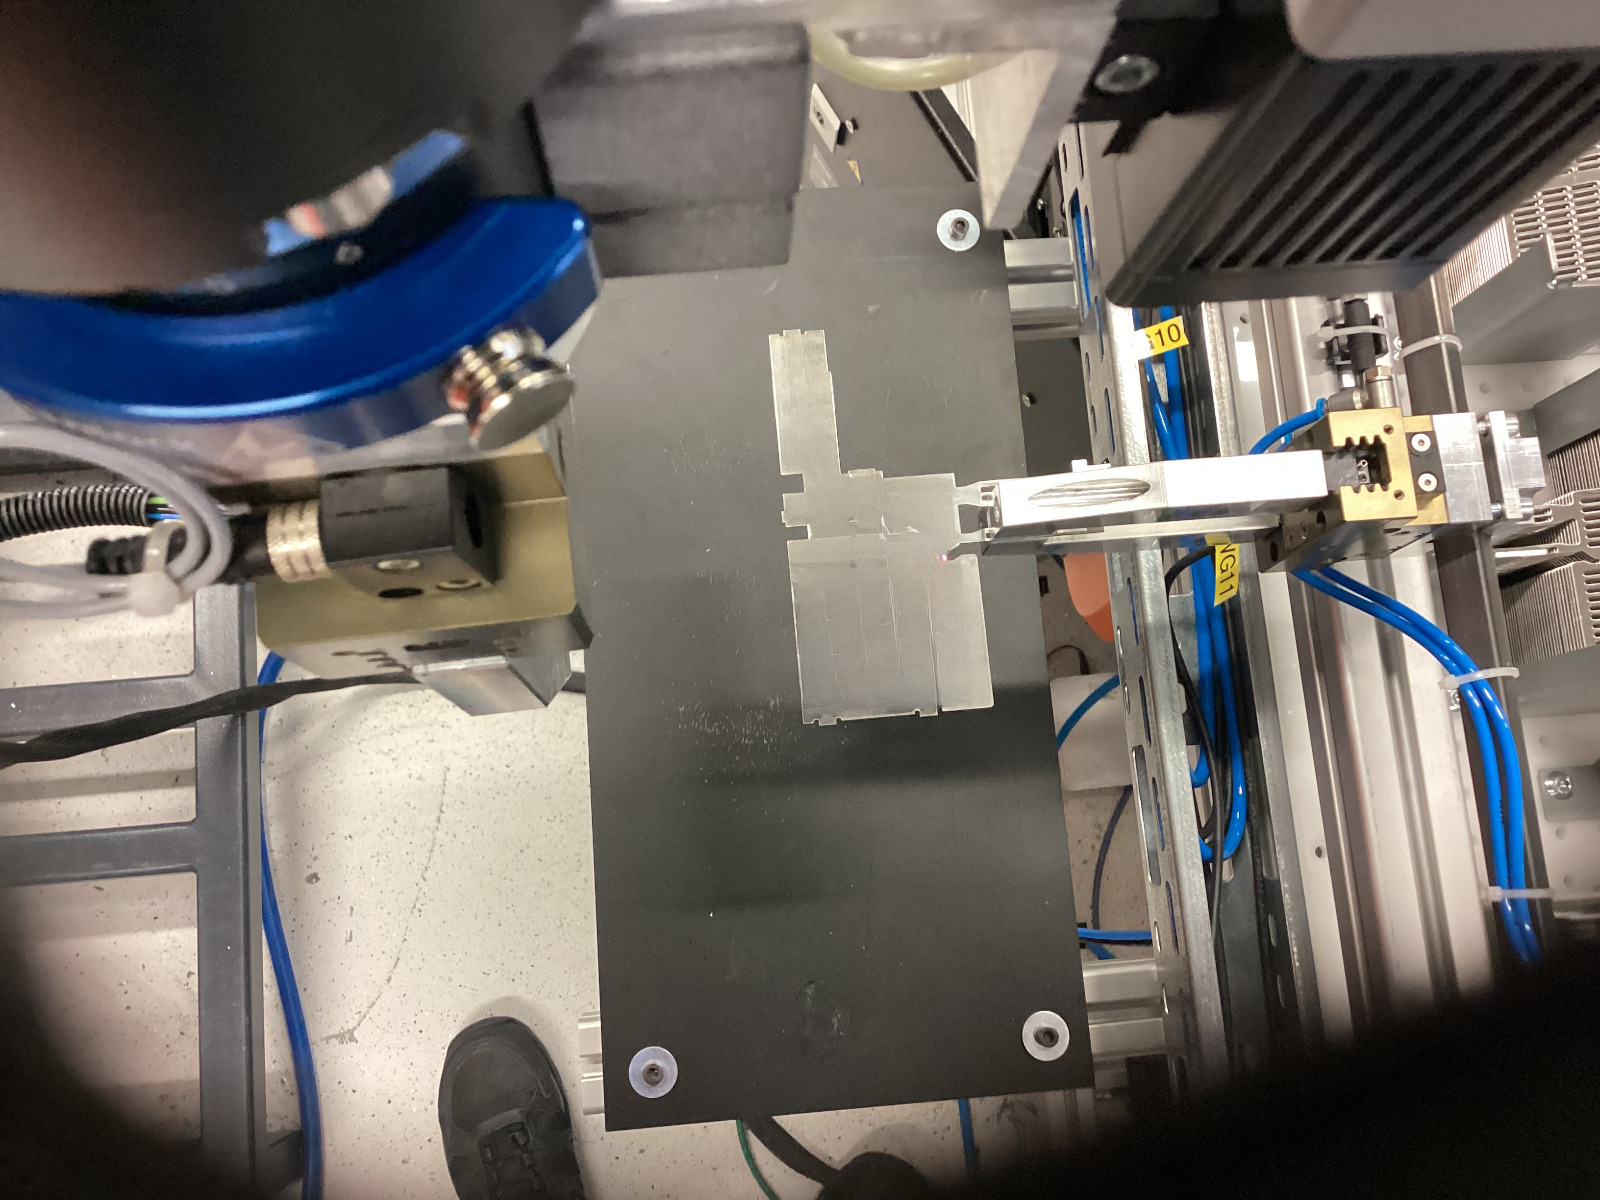
\includegraphics[width=\textwidth]{figures/sheet-pickup/scan.png}
        \caption{Scan sheet pattern using contour detector}
        \label{subfig:sheet-scan}
    \end{subfigure}\hspace{0.1cm}
    \begin{subfigure}[b]{0.48\textwidth}
        \centering
        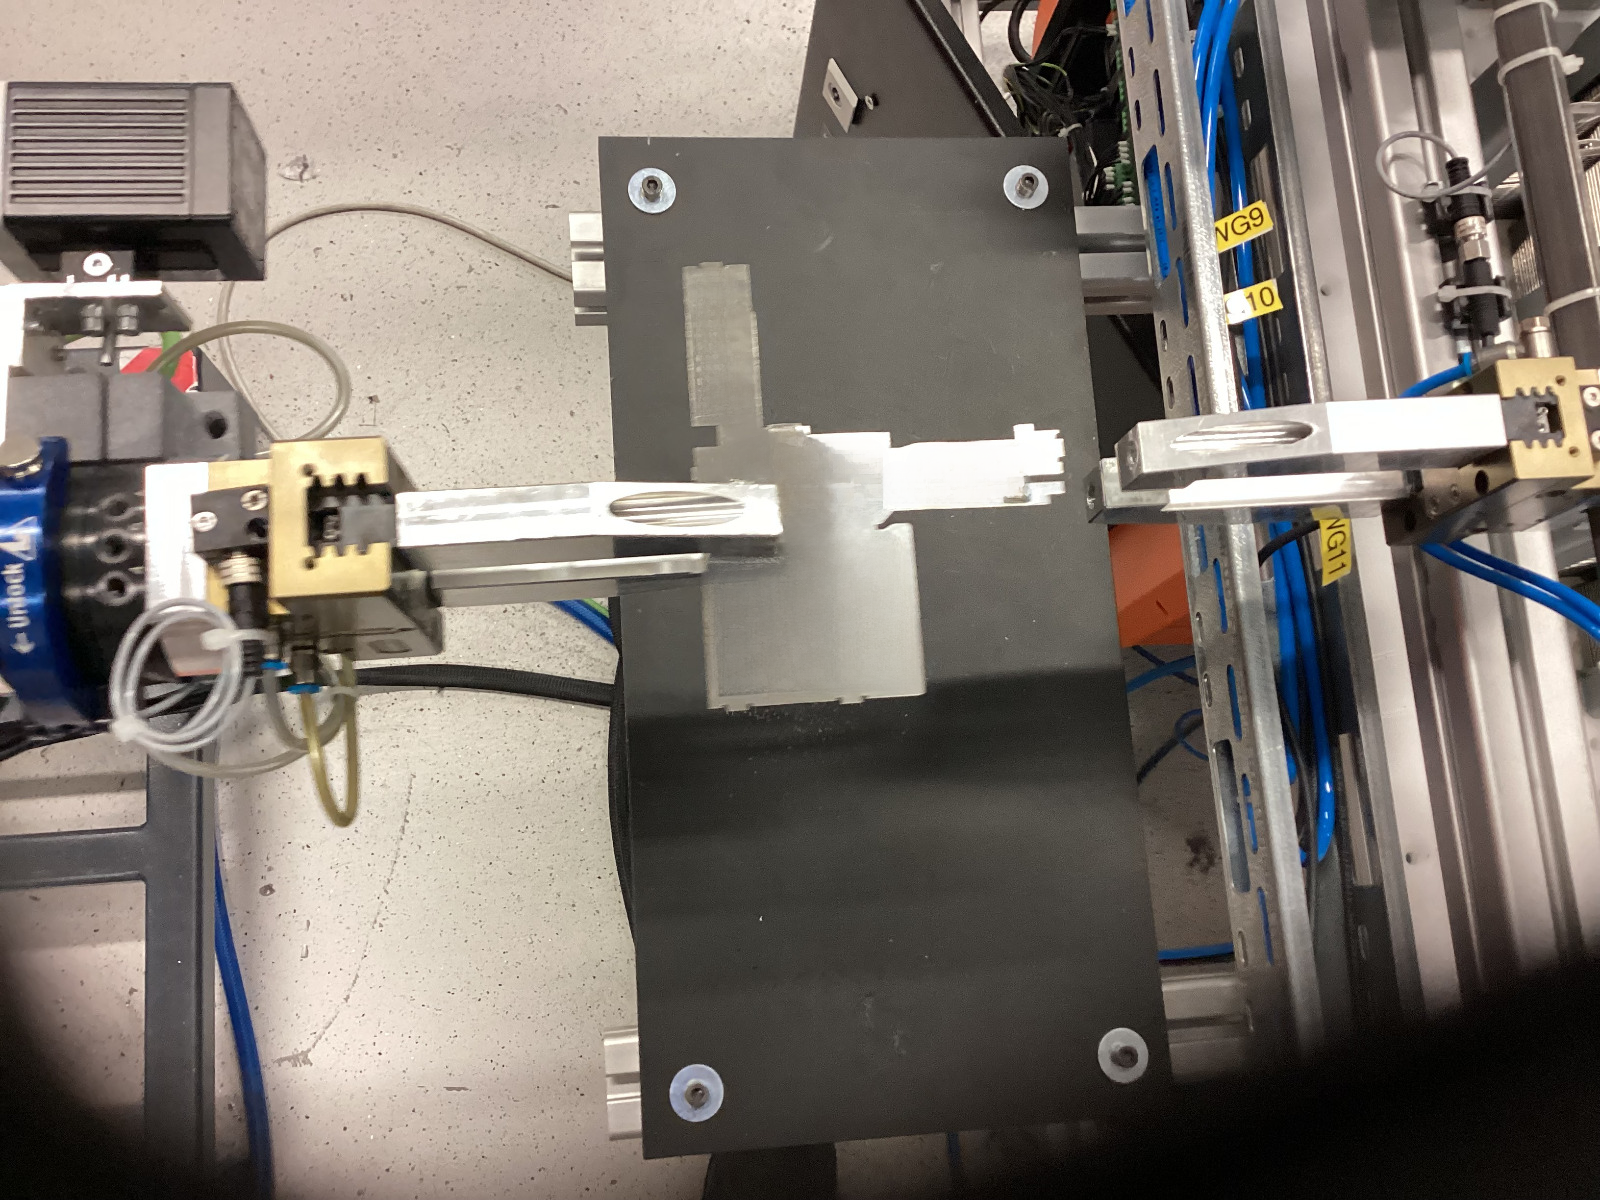
\includegraphics[width=\textwidth]{figures/sheet-pickup/taken.png}
        \caption{collect the sheet}
        \label{subfig:sheet-taken}
    \end{subfigure}
    \caption{Sheet pickup using robotic gripper}
    \label{fig:sheet-pickup}
\end{figure}

\begin{figure}[h]
    \centering
    \begin{subfigure}[b]{0.48\textwidth}
        \centering
        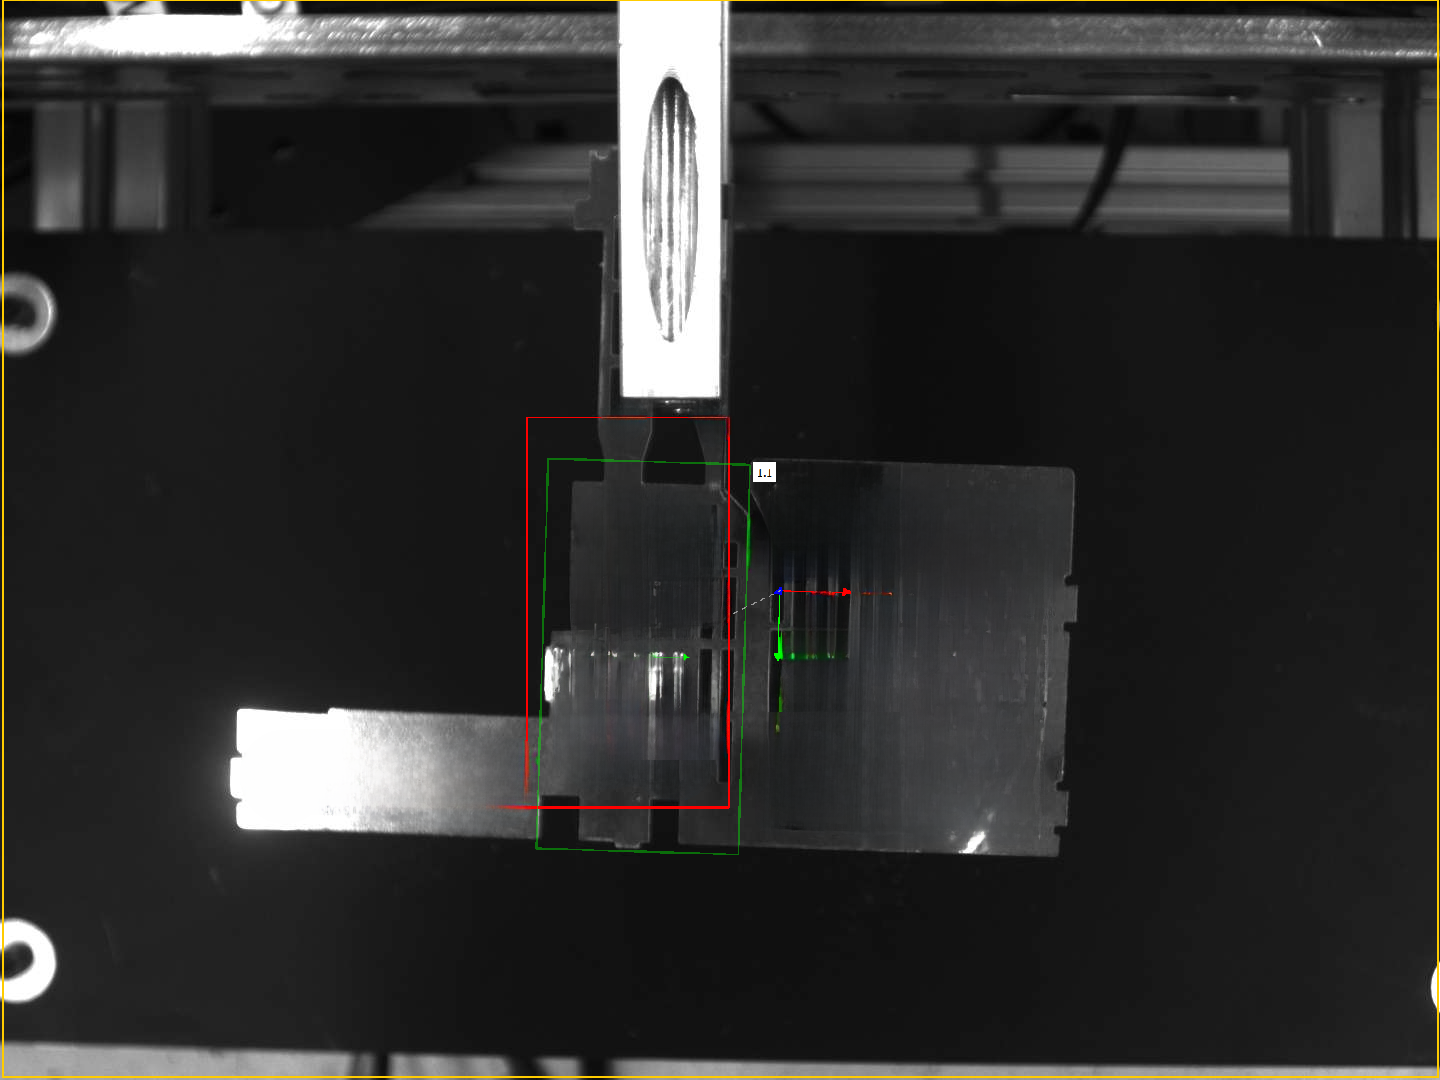
\includegraphics[width=\textwidth]{figures/sheet-pickup/camera-align.png}
        \caption{align camera}
        \label{subfig:sheet-1}
    \end{subfigure}\hspace{0.1cm}
    \begin{subfigure}[b]{0.48\textwidth}
        \centering
        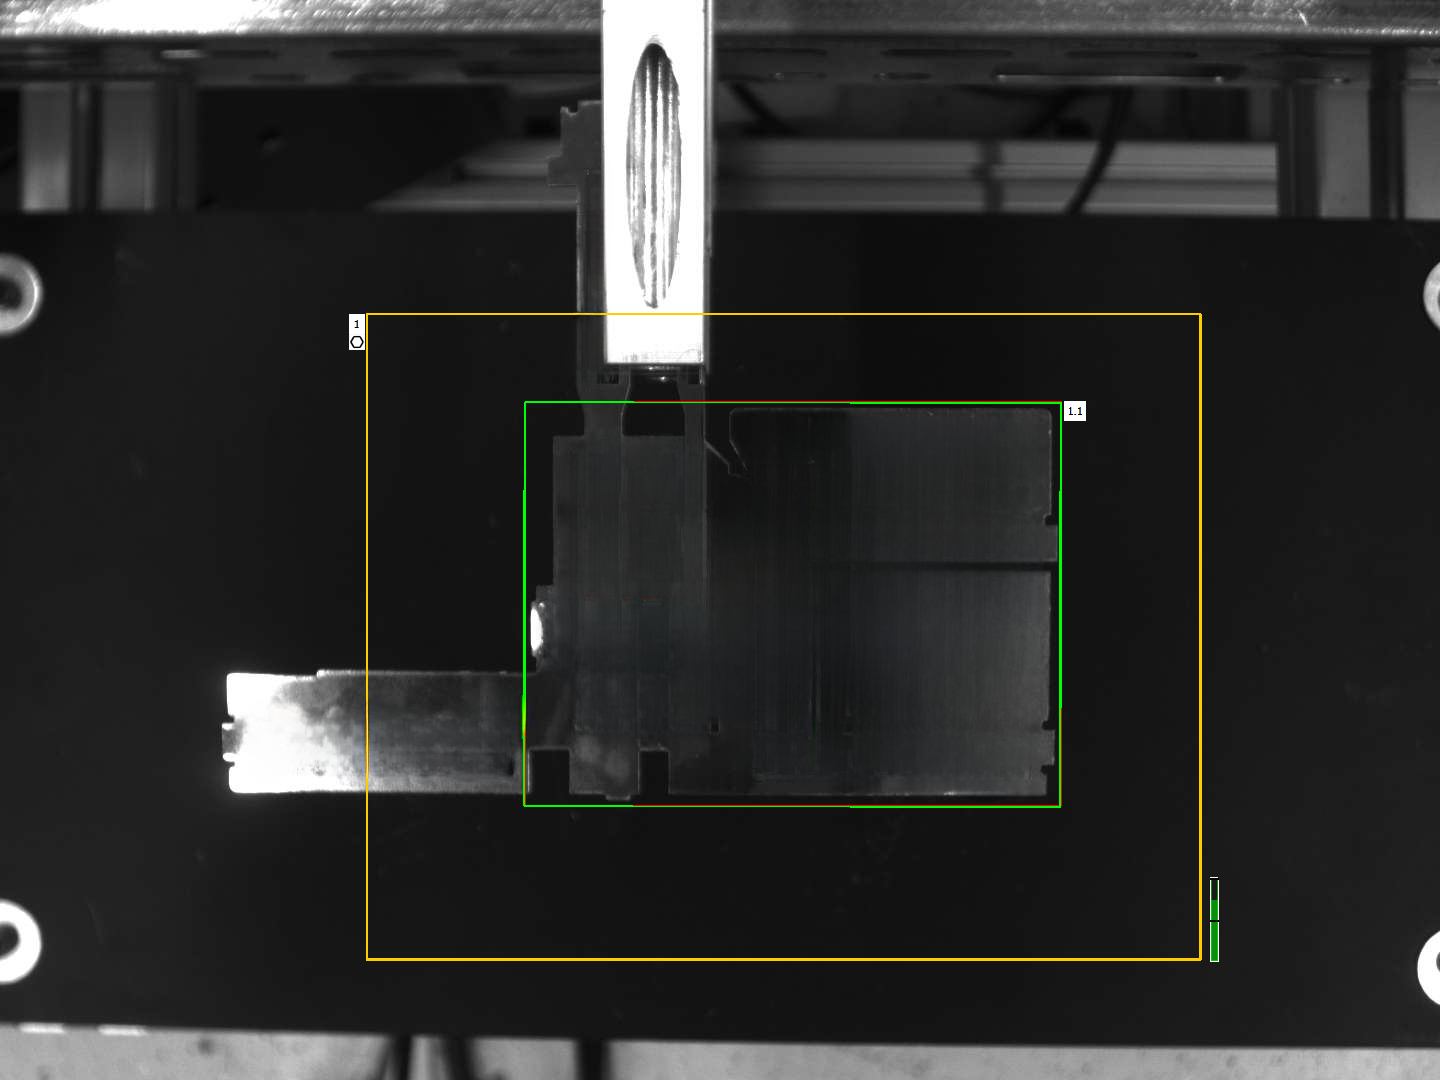
\includegraphics[width=\textwidth]{figures/sheet-pickup/sheet-pose.png}
        \caption{send sheet pose to pickup the sheet}
        \label{subfig:sheet-0}
    \end{subfigure}
    \caption{Sheet pattern detection using detector contour}
    \label{fig:sheet-scanning}
\end{figure}

The KR1410 uses the camera to detect and then securely pick the sheet. There are two stages of scanning as shown in figure \ref{fig:sheet-scanning}. A first scan aligns the camera perfectly with the sheet pattern. The second image capture detects the sheet with high accuracy in this way and sends the pose to the robot in world frame as shown in figure \ref{fig:sensoconfig-pattern}. Both stages uses detector contour to get the sheet pose.
The accuracy of the pickup is crucial for the success of the subsequent bending operations. Any misalignment at this stage could lead to errors in the final dimensions of the bent part.

\begin{figure}[h]
    \centering
    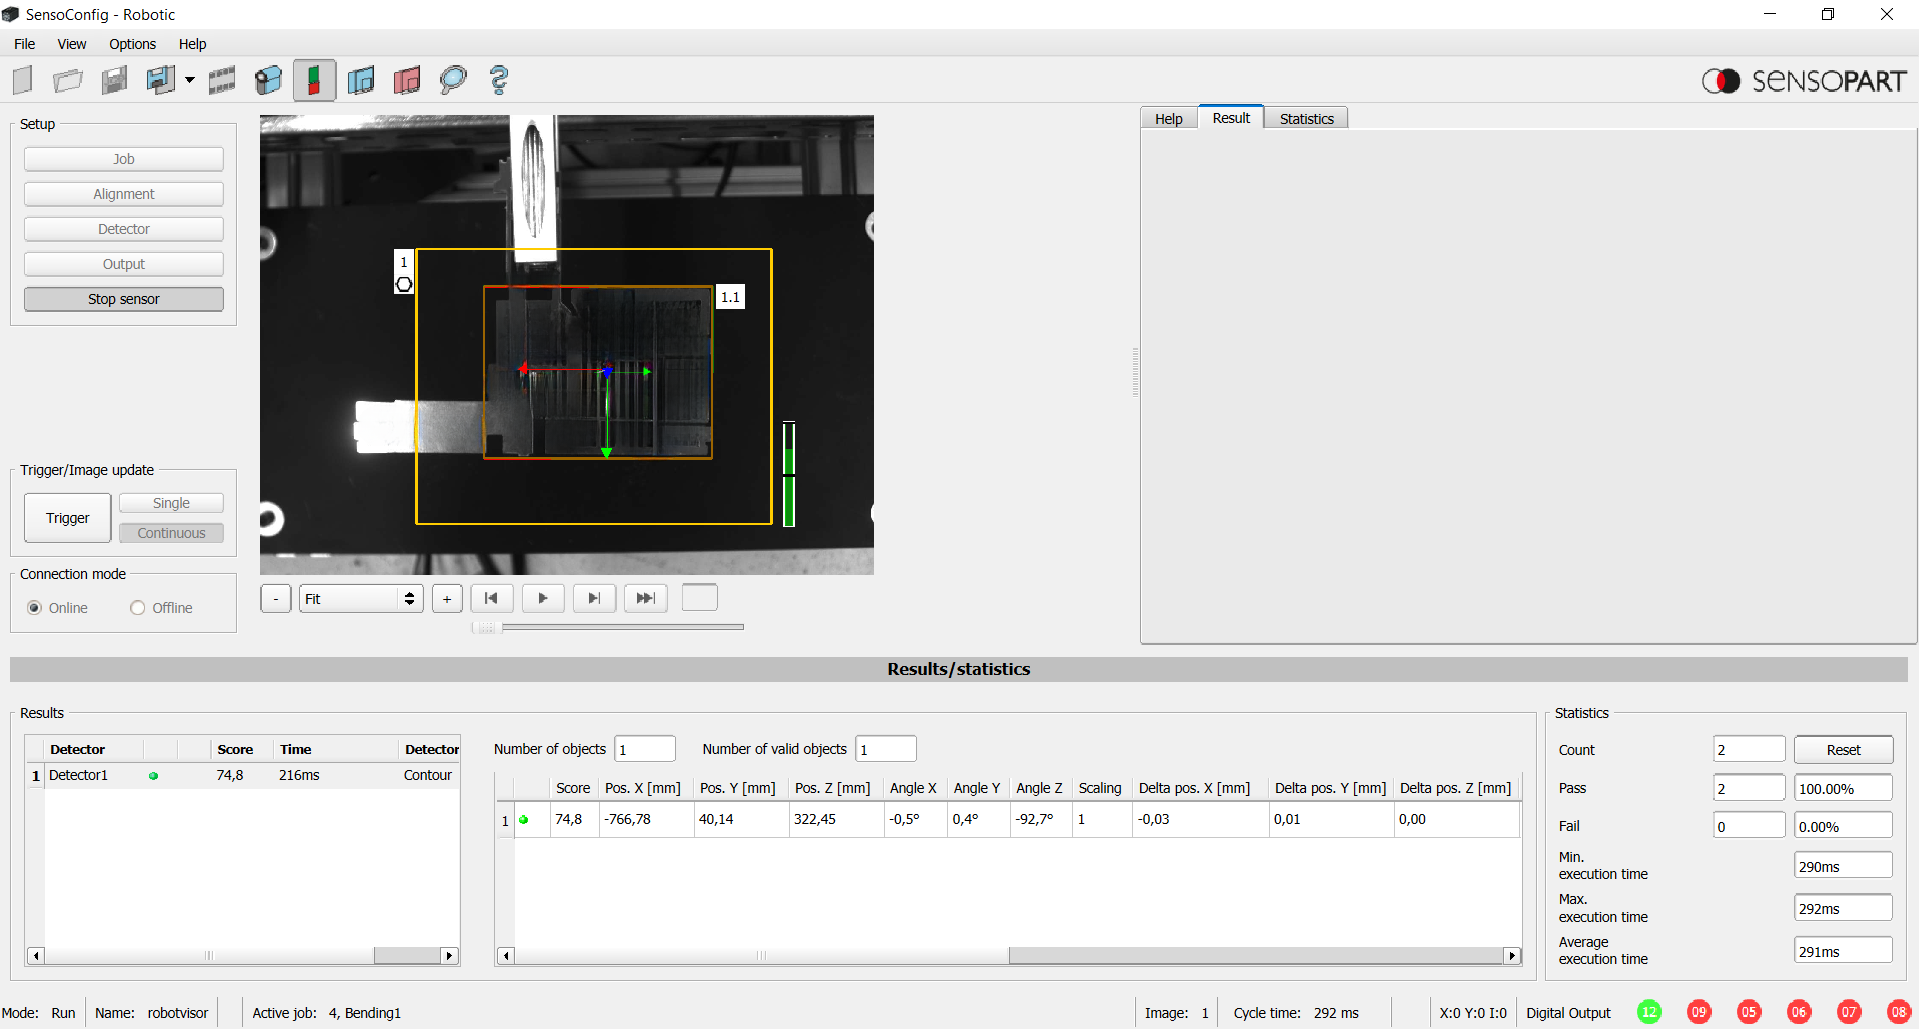
\includegraphics[width=\textwidth]{figures/sheet-pickup/sensoconfig.PNG}
    \caption{Detection and sending of sheet pose using telegram (SensoConfig)}
    \label{fig:sensoconfig-pattern}
\end{figure}

In some instances, to avoid collisions during next bending operation or for better handling of part, regripping of the sheet from a different position is required. This is where the unloading station gripper plays a crucial role in repositioning the sheet. The unloading station gripper is controlled from the KR1410 robot if the robot program state Int[0] is $\ge$3. (See table \ref{tab:kr1410-to-plc}). Otherwise the unloading station gripper is controlled by the PLC. 
\vspace{1\baselineskip}

First, the robot transfers the bent sheet to the unloading station gripper. Then, it is the same process as the sheet pickup in the first step of the bending cycle. The robot moves to the scanning pose, scans and aligns with the sheet, detects and grips the sheet and finally move out the part from the unloading station gripper.
Figure \ref{fig:sheet-pickup-before-placement} illustrates the step-by-step process of regrasping of sheet metal part for sheet placement in the storage station after all the bending operations are complete.


\begin{figure}[h]
    \centering
    \begin{subfigure}[b]{0.32\textwidth}
        \centering
        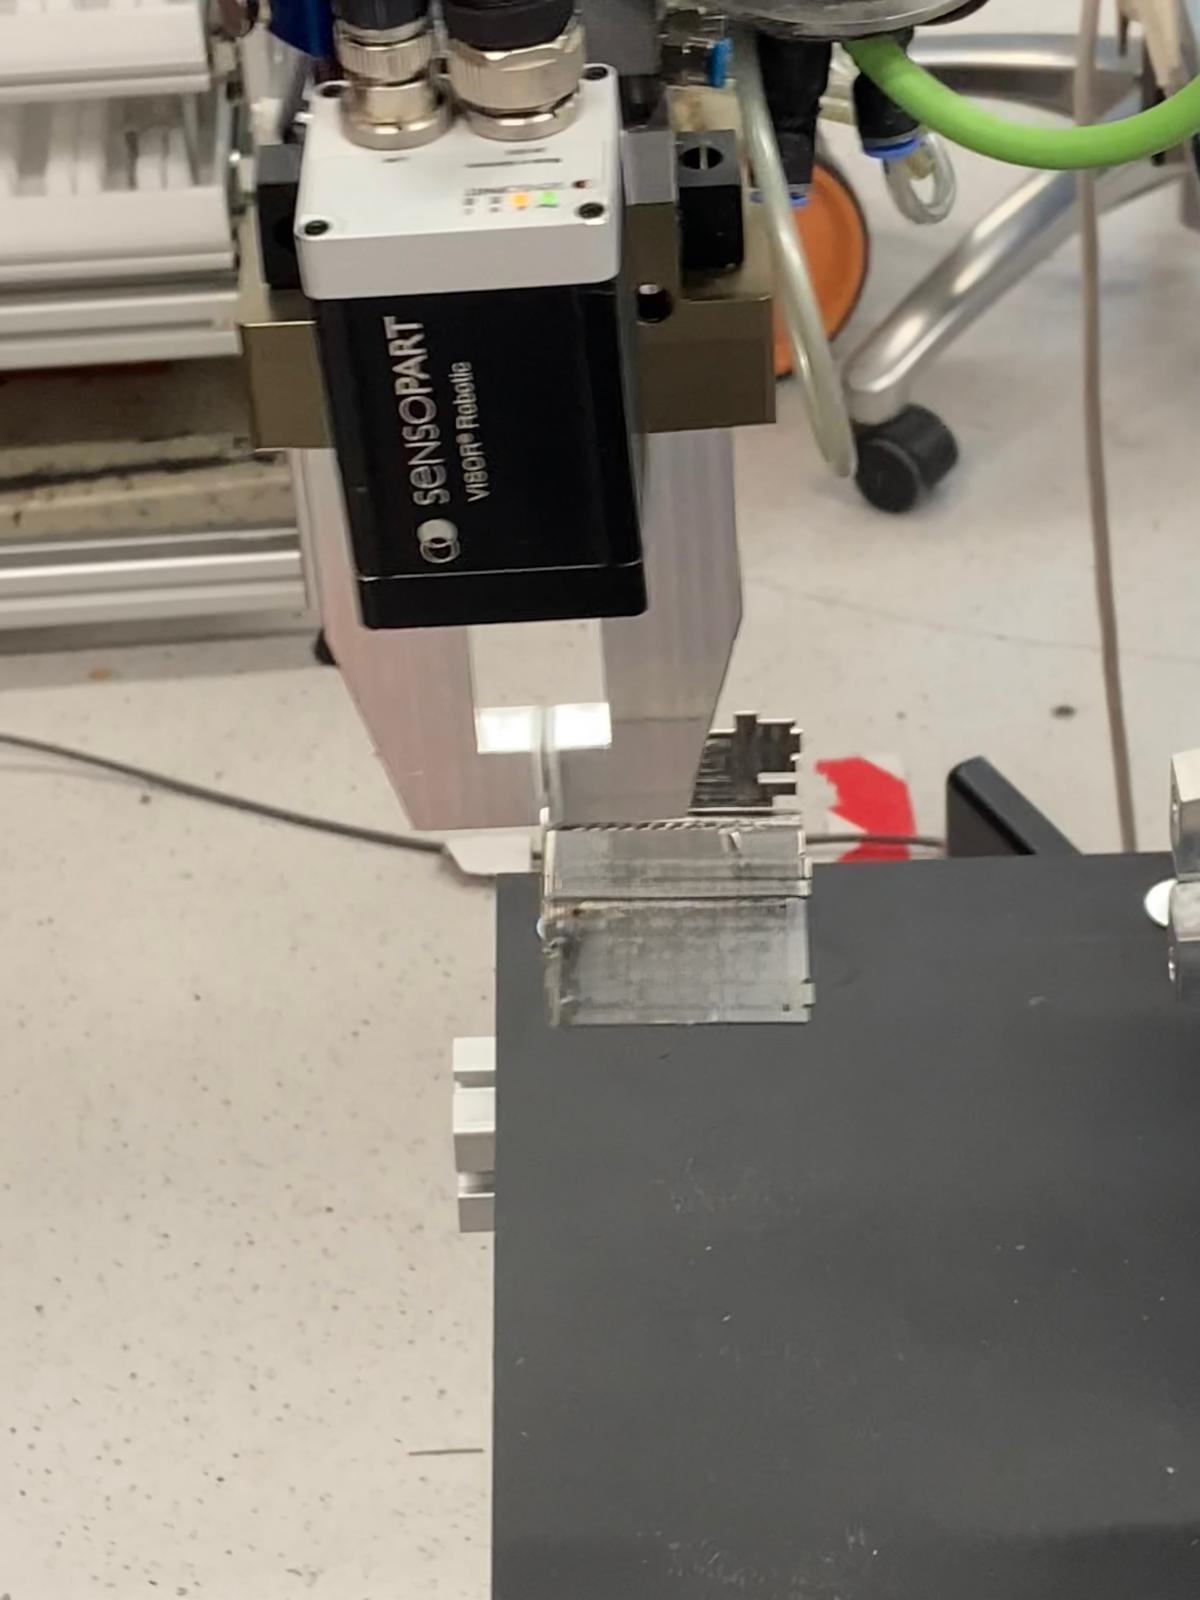
\includegraphics[width=\textwidth]{figures/sheet-pickup/sheet-placement01.png}
        \caption{Go to unloading station gripper}
        \label{subfig:sheet-placement01}
    \end{subfigure}\hspace{0.1cm}
    \begin{subfigure}[b]{0.32\textwidth}
        \centering
        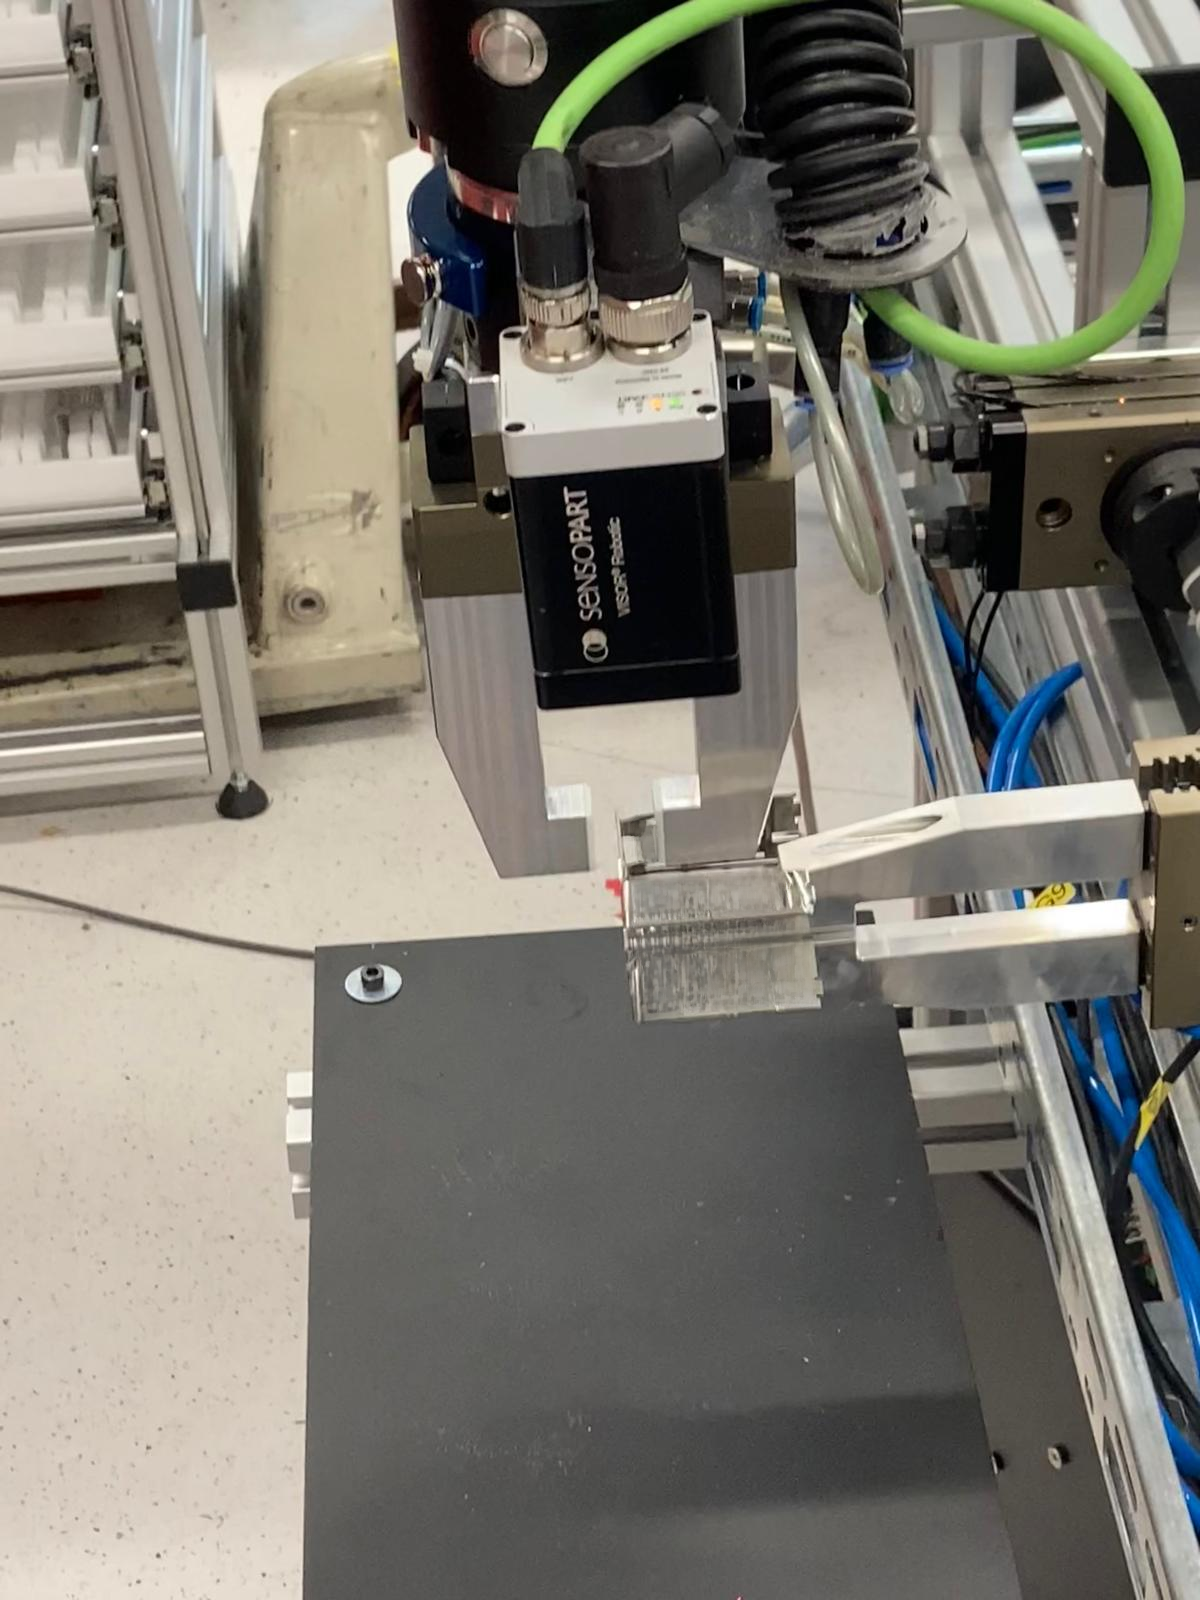
\includegraphics[width=\textwidth]{figures/sheet-pickup/sheet-placement02.png}
        \caption{transfer sheet to unloading station gripper}
        \label{subfig:sheet-placement02}
    \end{subfigure}\hspace{0.1cm}
    \vspace{1cm}
    \begin{subfigure}[b]{0.32\textwidth}
        \centering
        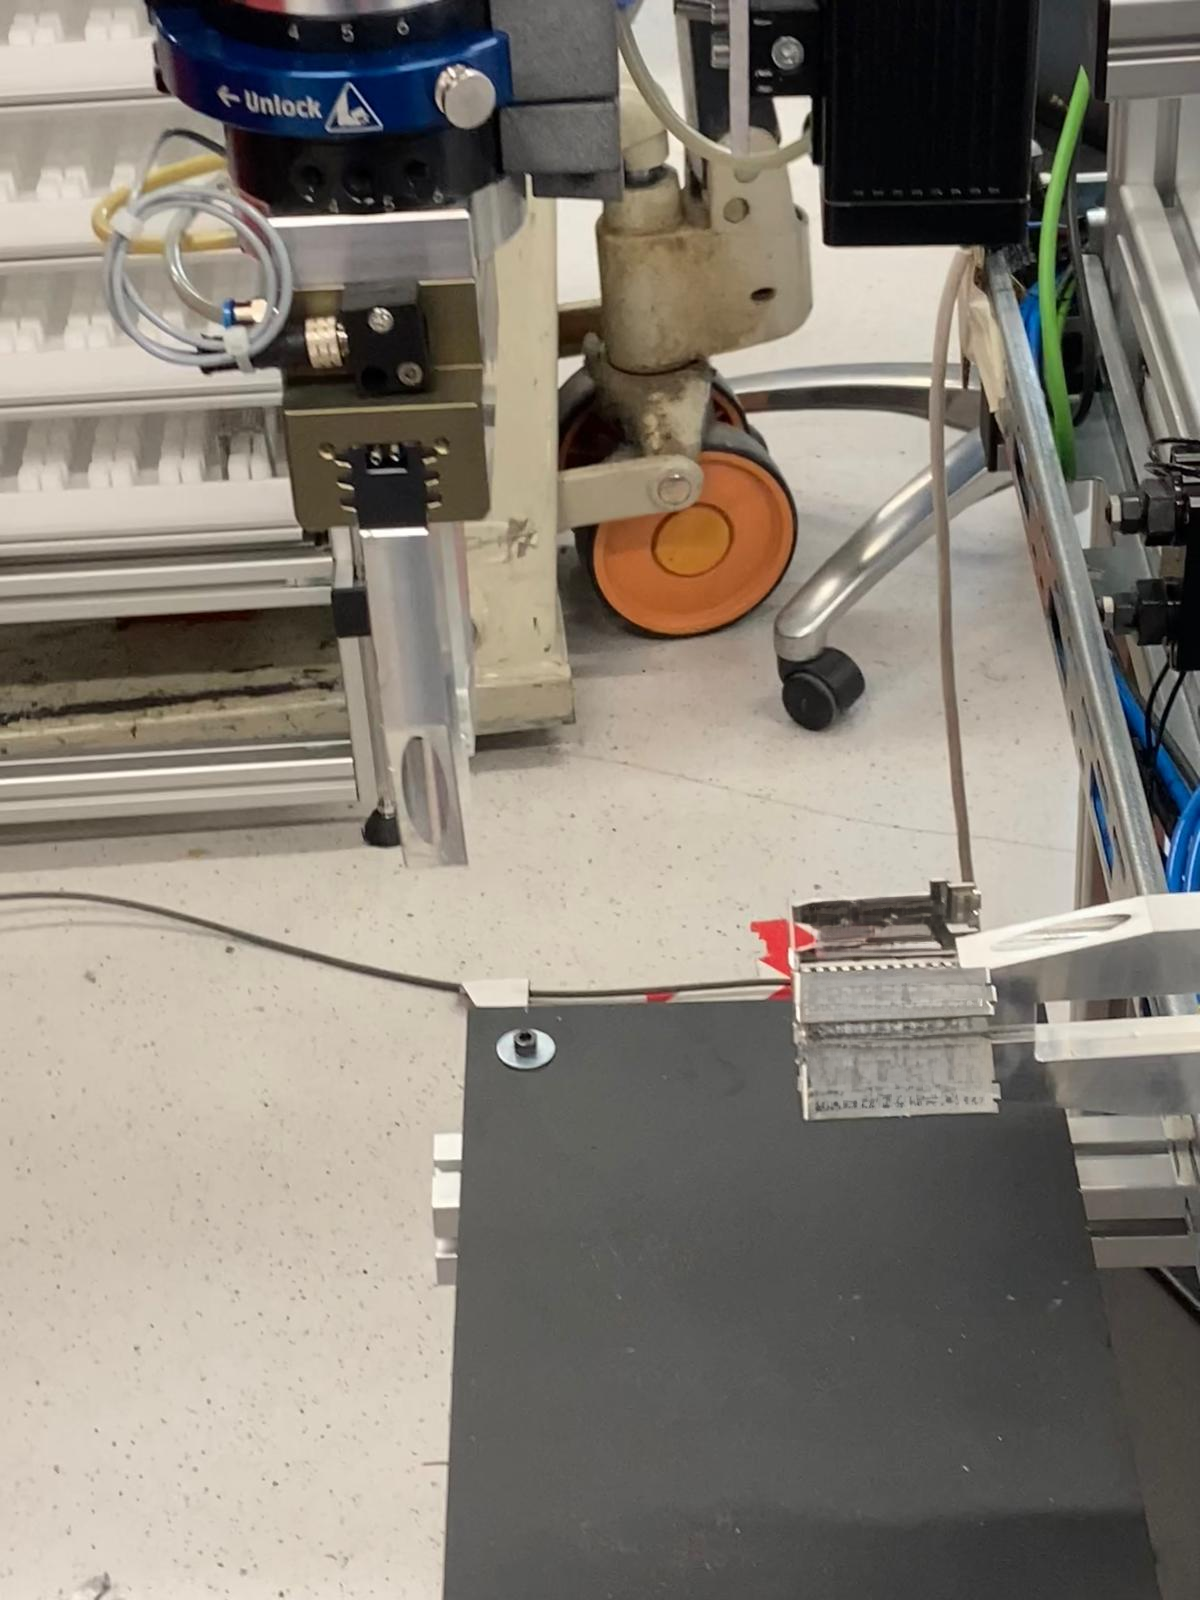
\includegraphics[width=\textwidth]{figures/sheet-pickup/sheet-placement03.png}
        \caption{Scan sheet pattern and align camera}
        % \vspace{-0.45cm}
        \label{subfig:sheet-placement03}
    \end{subfigure}\hspace{0.1cm}
    \begin{subfigure}[b]{0.32\textwidth}
        \centering
        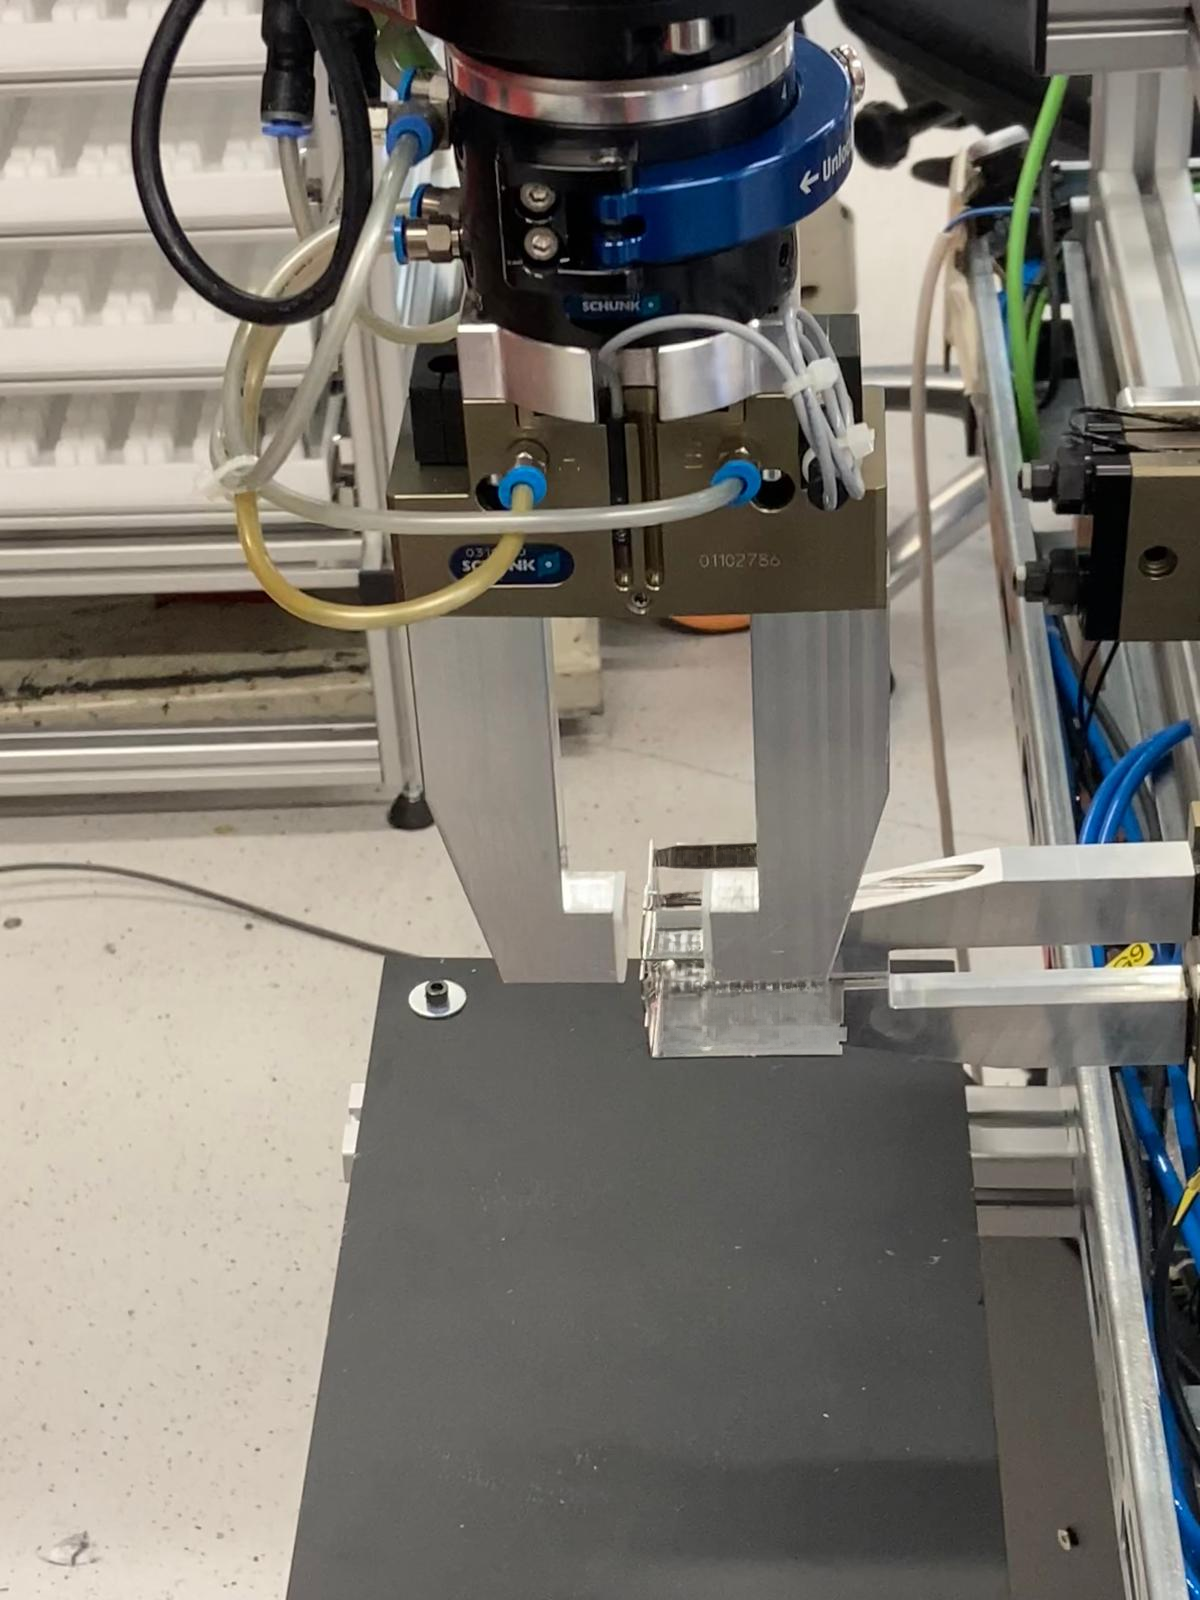
\includegraphics[width=\textwidth]{figures/sheet-pickup/sheet-placement04.png}
        \caption{Scan again for sheet detection}
        \label{subfig:sheet-placement04}
    \end{subfigure}\hspace{0.1cm}
    \vspace{0.75cm}
    \begin{subfigure}[b]{0.32\textwidth}
        \centering
        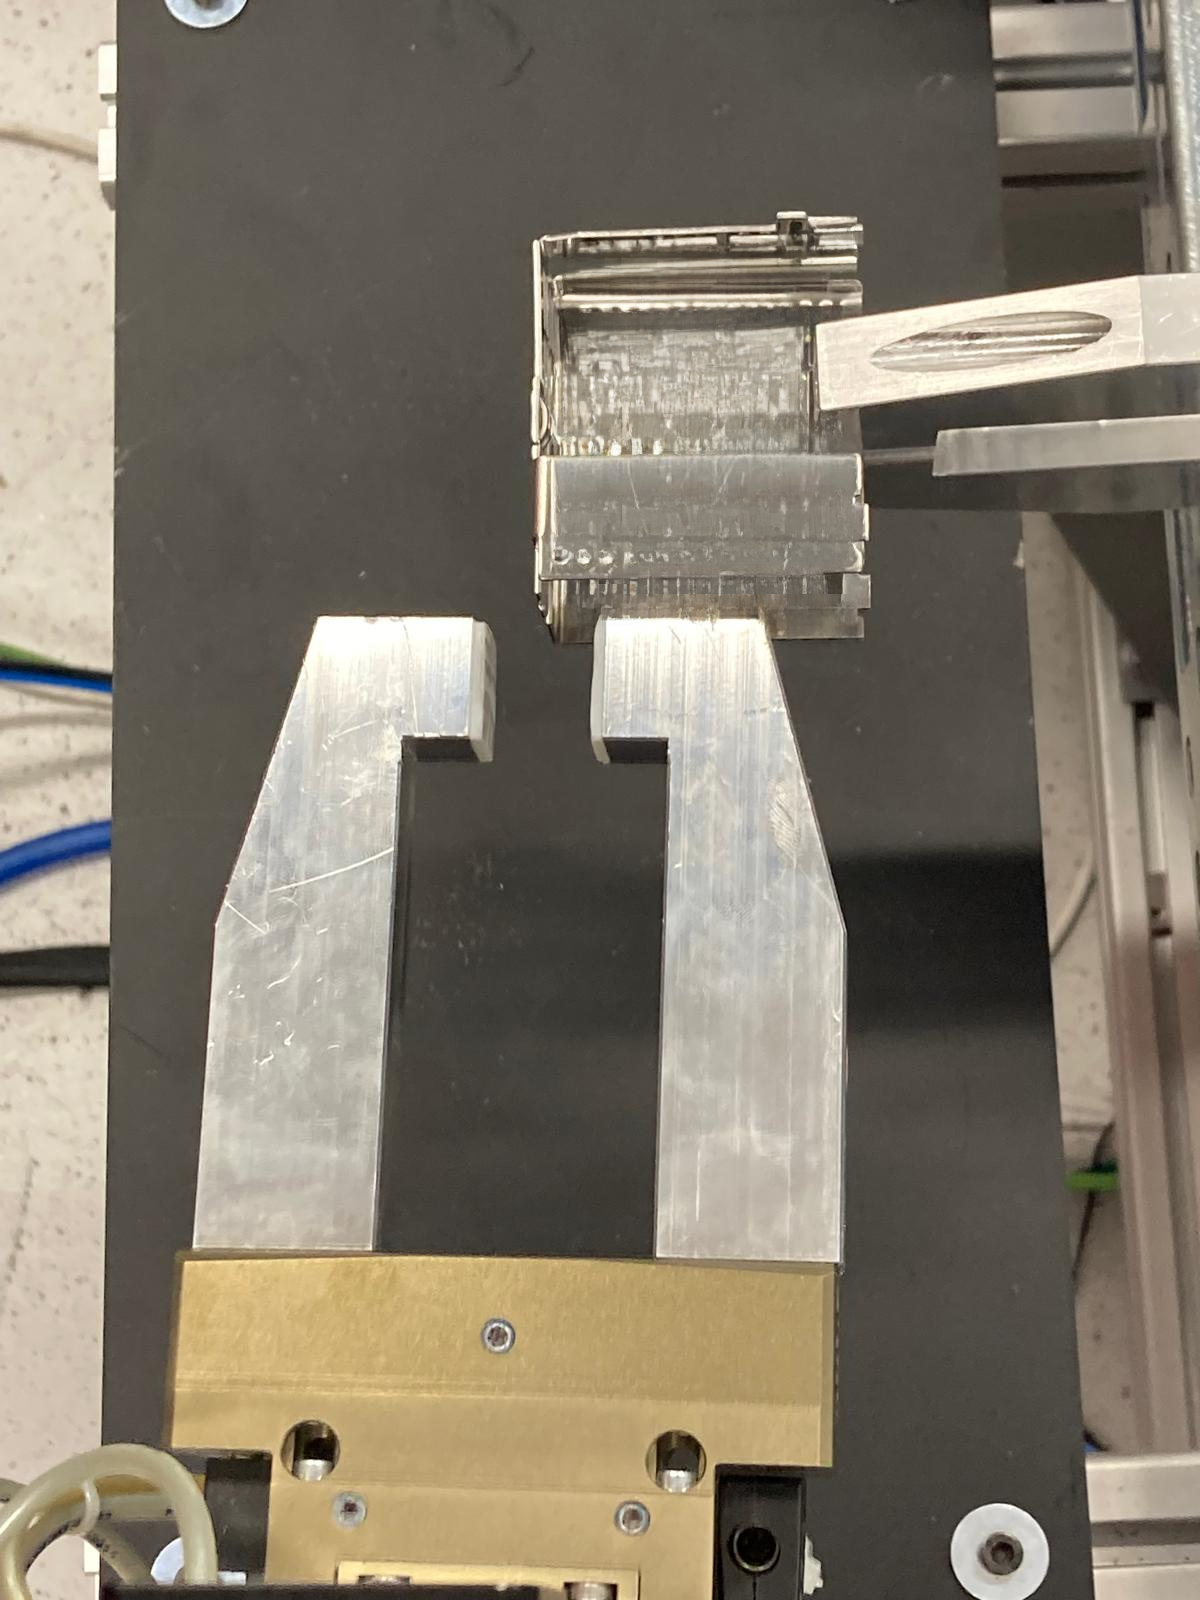
\includegraphics[width=\textwidth]{figures/sheet-pickup/sheet-placement05.png}
        \caption{Grasp sheet from unloading station gripper}
        \label{subfig:sheet-placement05}
    \end{subfigure}\hspace{0.1cm}
    \begin{subfigure}[b]{0.32\textwidth}
        \centering
        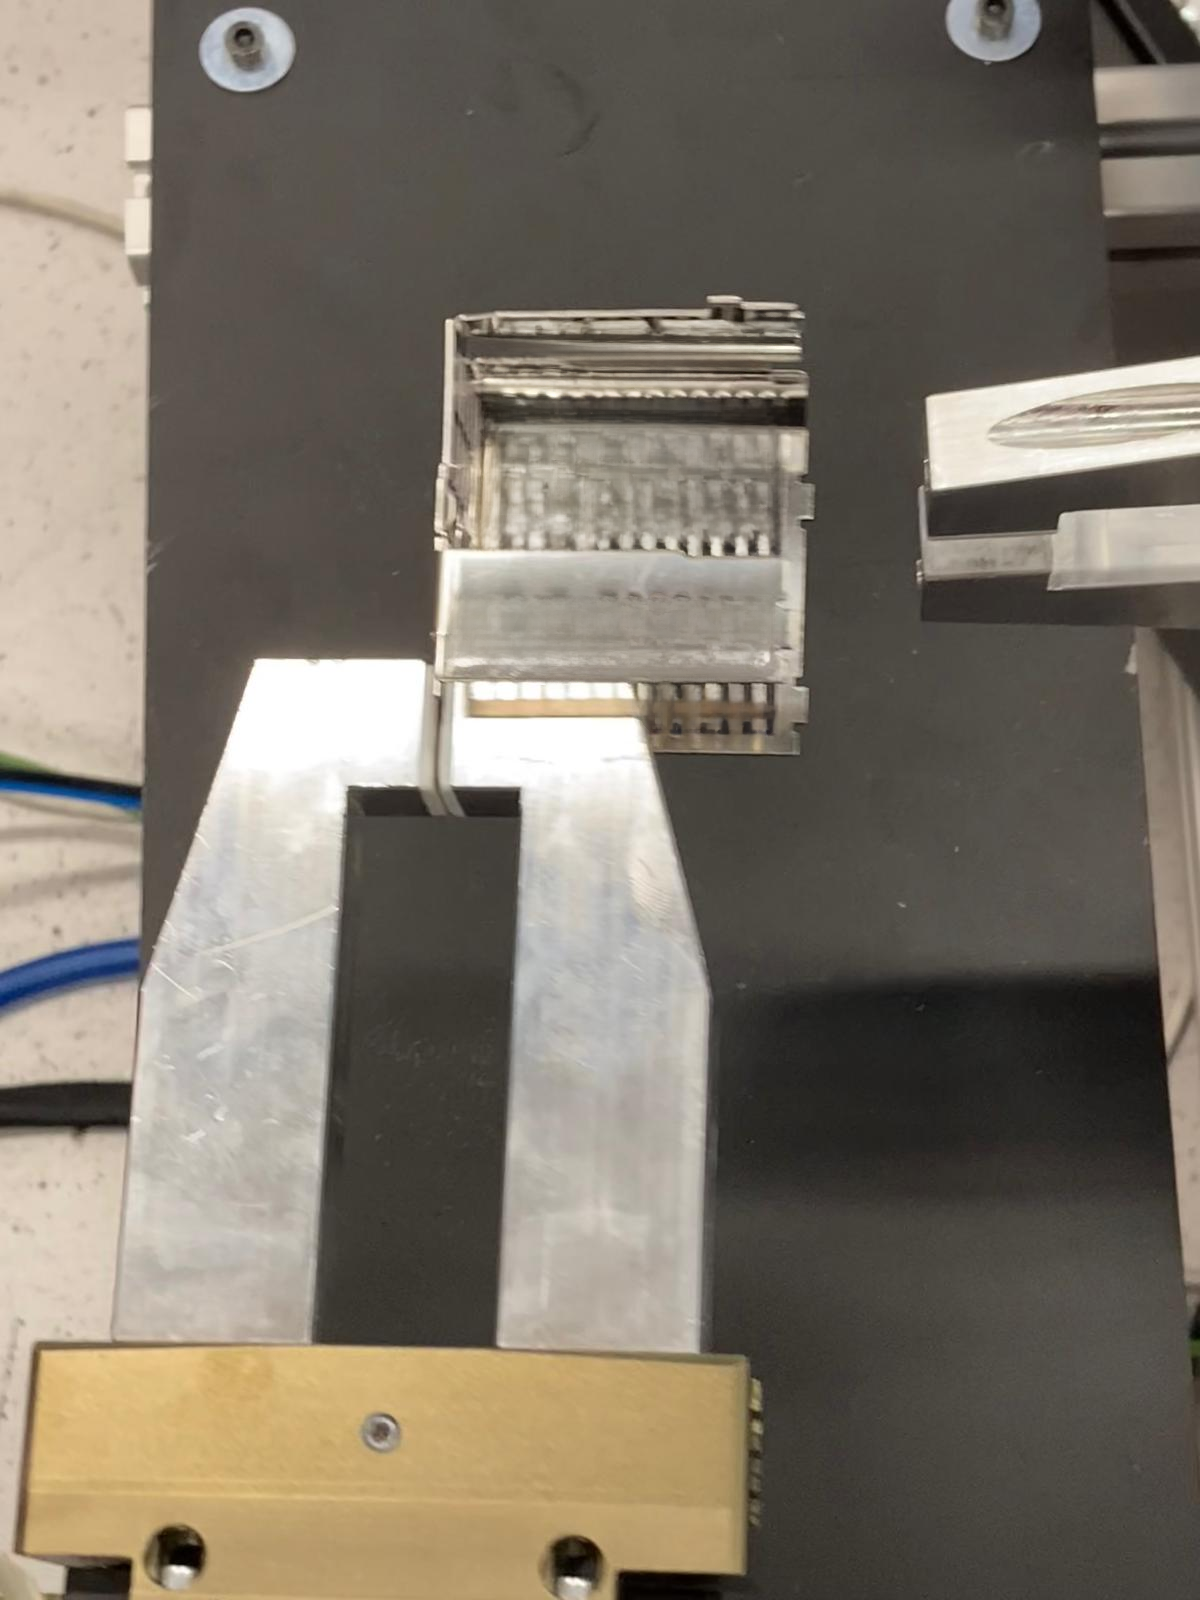
\includegraphics[width=\textwidth]{figures/sheet-pickup/sheet-placement06.png}
        \caption{Move out}
        \label{subfig:sheet-placement06}
        \vspace{0.45cm}
    \end{subfigure}\hspace{0.1cm}
    \caption{Regrasping bent sheet from a different position before placement in drawer}
    \label{fig:sheet-pickup-before-placement}
\end{figure}


\subsection{Bending Operation}
\label{subsec:bending-operation}
% Bending operations

The test part undergoes a sequence of six bendings, with different angles and setups. Specifically, bending operations 1, 5, and 6 are performed at bending station 1 and undergoes a bending of 90° angle, whereas bending operations 2 and 3 are performed at bending station 2 with a bending of 135°, and the fourth bending operation is simply done to flatten the sheet metal part.

The first step before the bending for all bending operations is the correct alignment of the part in the backgauges of the bending machine. The bending machine program is automatically set by the terminal operating robot. Once the correct sequence is selected in the terminal of the bending machine, PLC send a signal to the KR1410 robot which gives permission to align the sheet in the backgauges.
Then only the KR1410 arm secures the part in the backgauges of the bending machine.

\begin{figure}[h]
    \centering
    \begin{subfigure}[b]{0.32\textwidth}
        \centering
        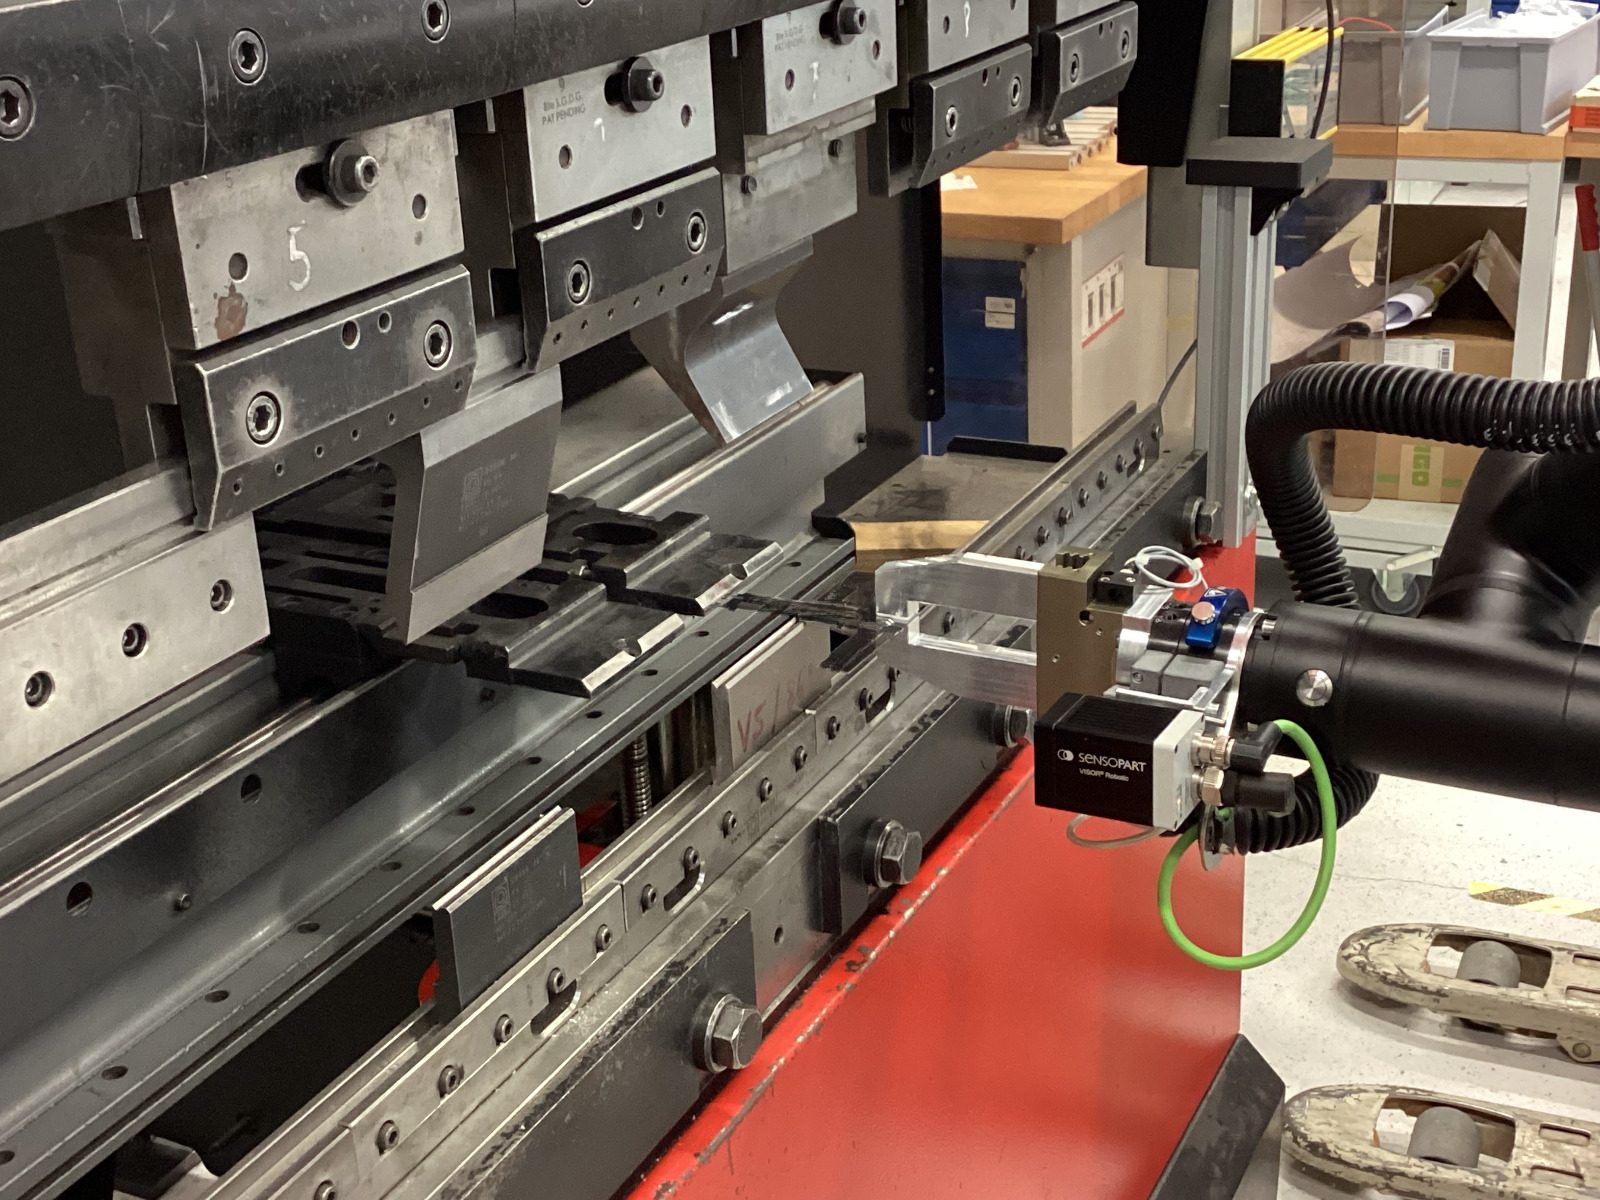
\includegraphics[width=\textwidth]{figures/bending/bending1-002.png}
        \caption{Go to bending station 1}
        \label{subfig:bending1-before}
    \end{subfigure}\hspace{0.1cm}
    \begin{subfigure}[b]{0.32\textwidth}
        \centering
        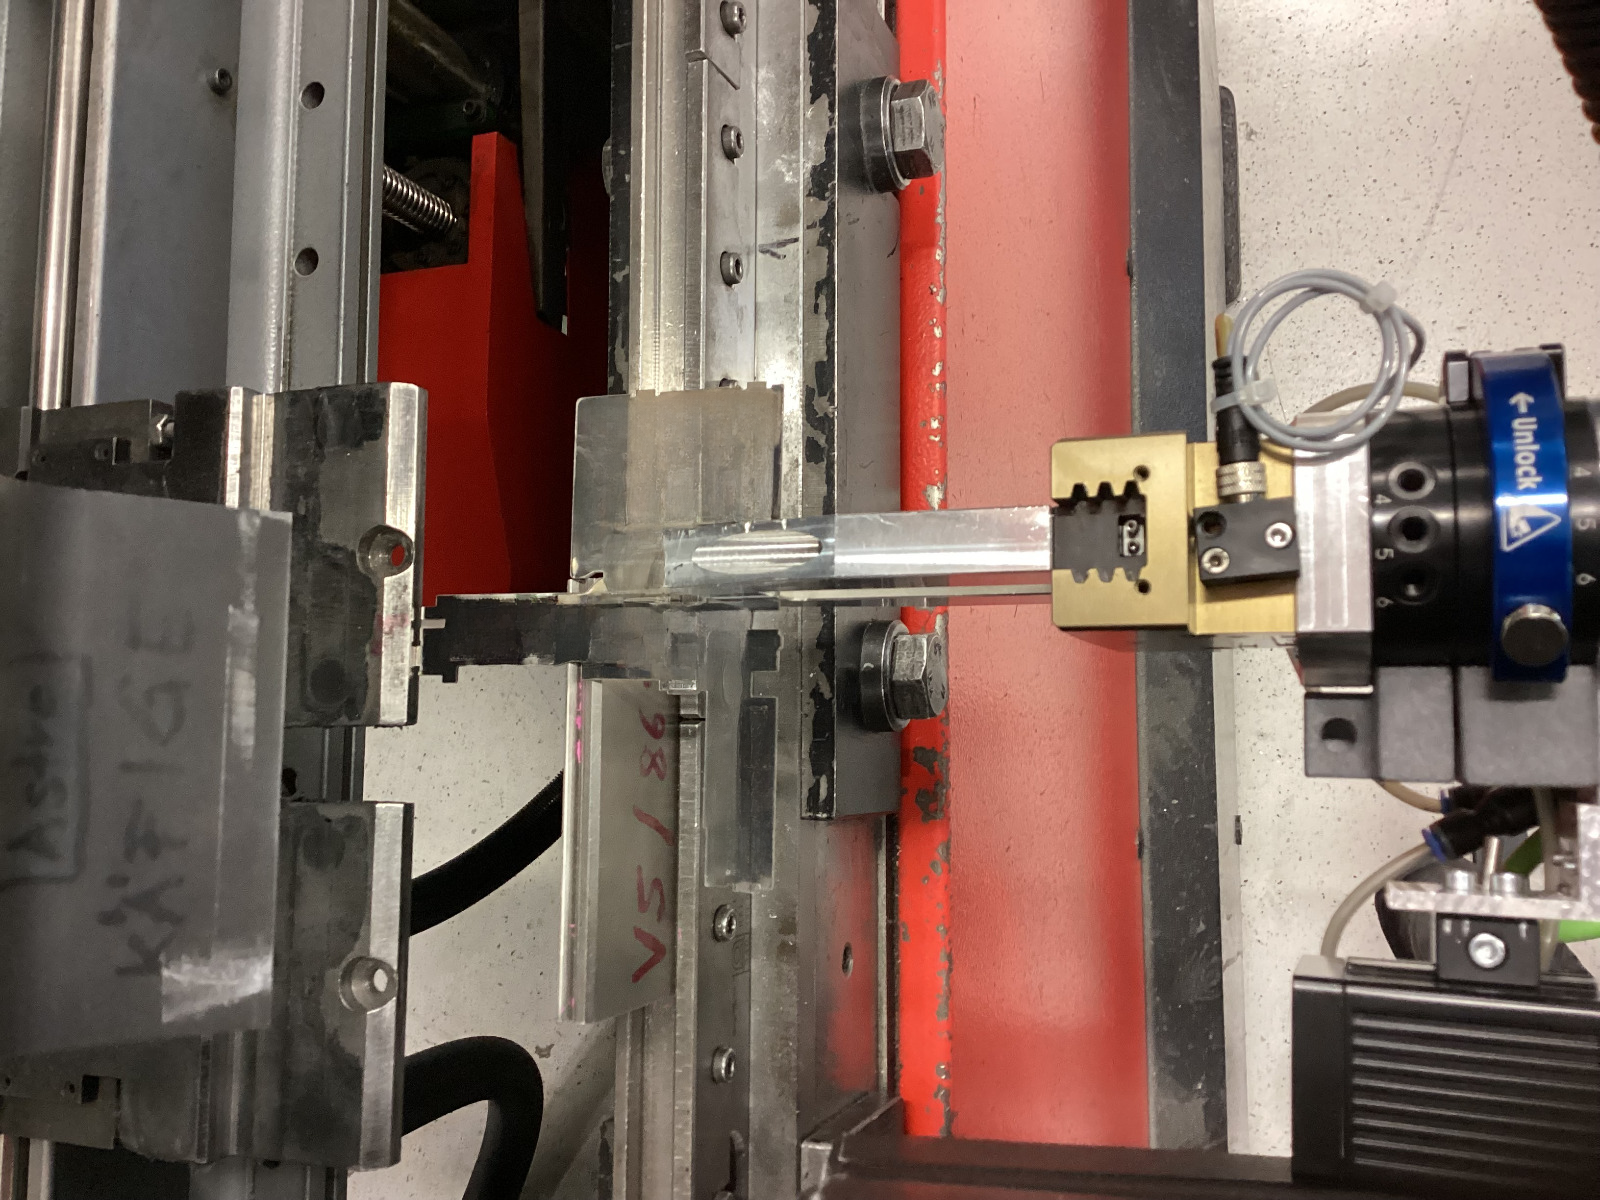
\includegraphics[width=\textwidth]{figures/bending/bending1-003.png}
        \caption{bend the sheet metal part}
        \label{subfig:bending1}
    \end{subfigure}\hspace{0.1cm}
    \begin{subfigure}[b]{0.32\textwidth}
        \centering
        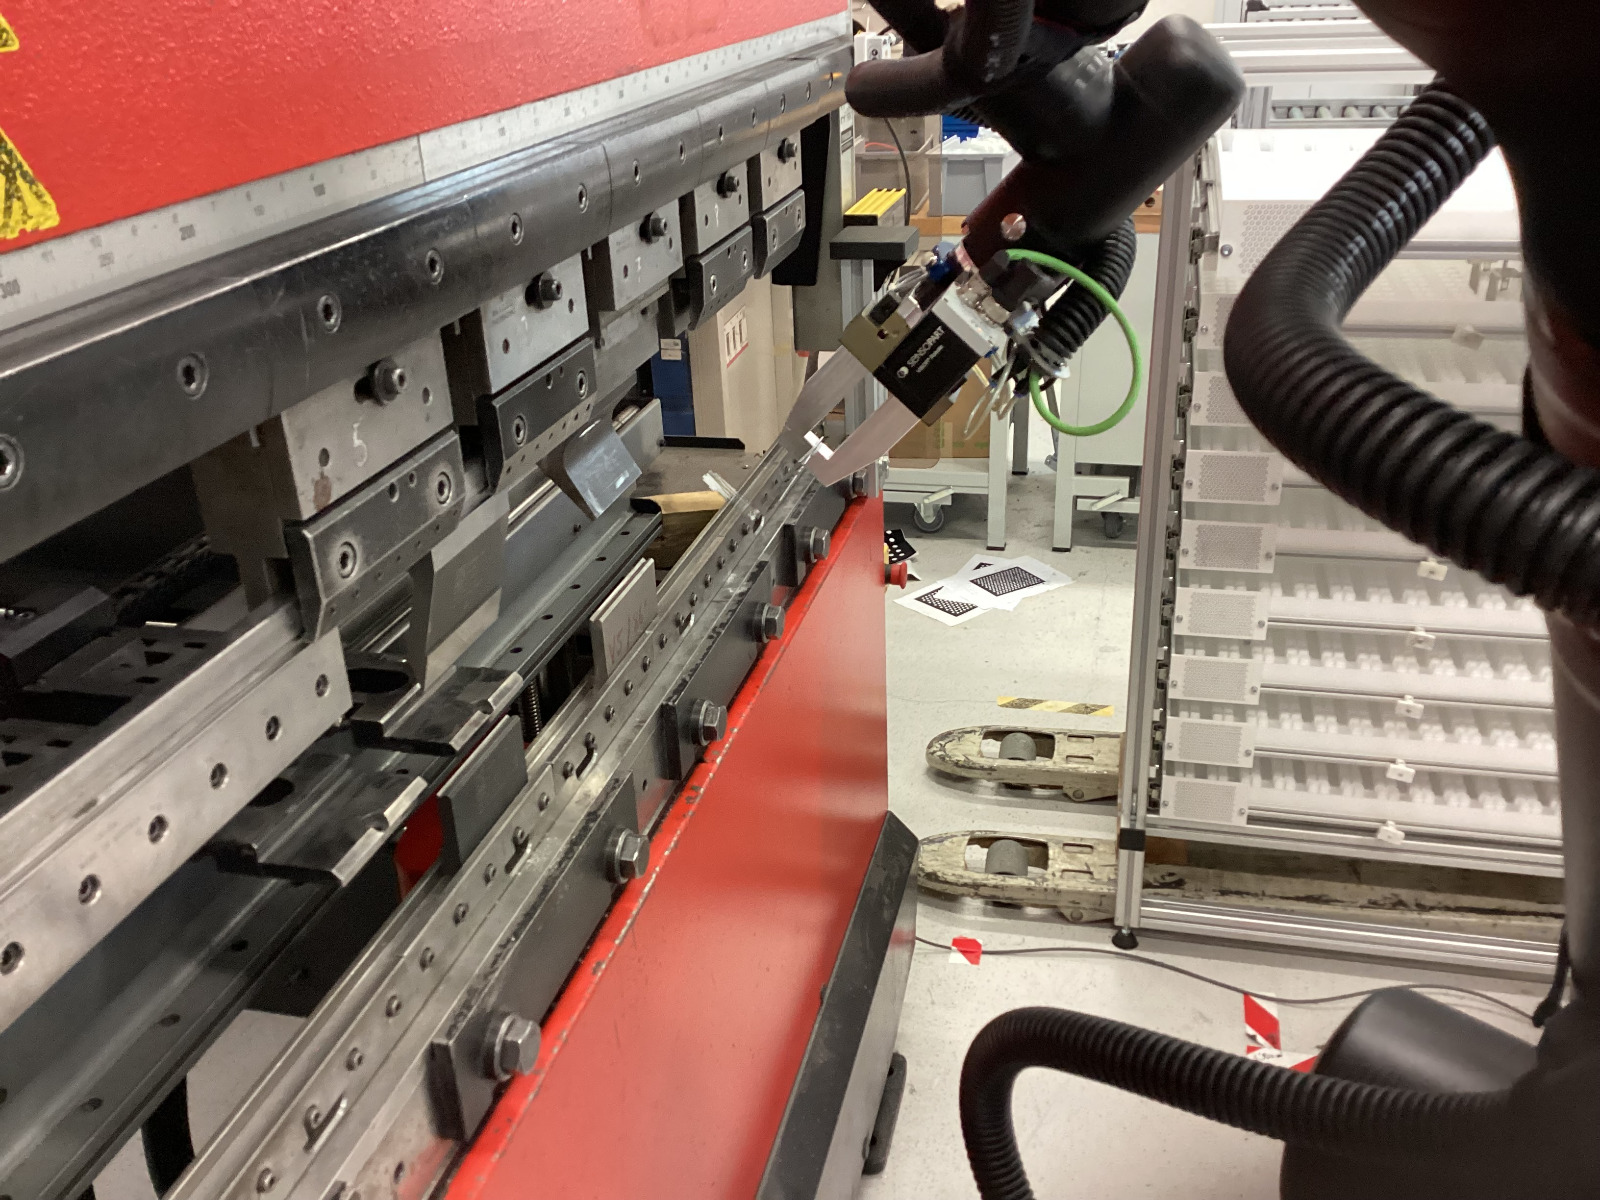
\includegraphics[width=\textwidth]{figures/bending/bending1-001.png}
        \caption{take away the bent sheet}
        \label{subfig:bending1-after}
    \end{subfigure}\hspace{0.1cm}
    \caption{Bending operation number 1 at bending station 1}
    \label{fig:bending-operation-1}
\end{figure}

\begin{figure}[h]
    \centering
    \begin{subfigure}[b]{0.32\textwidth}
        \centering
        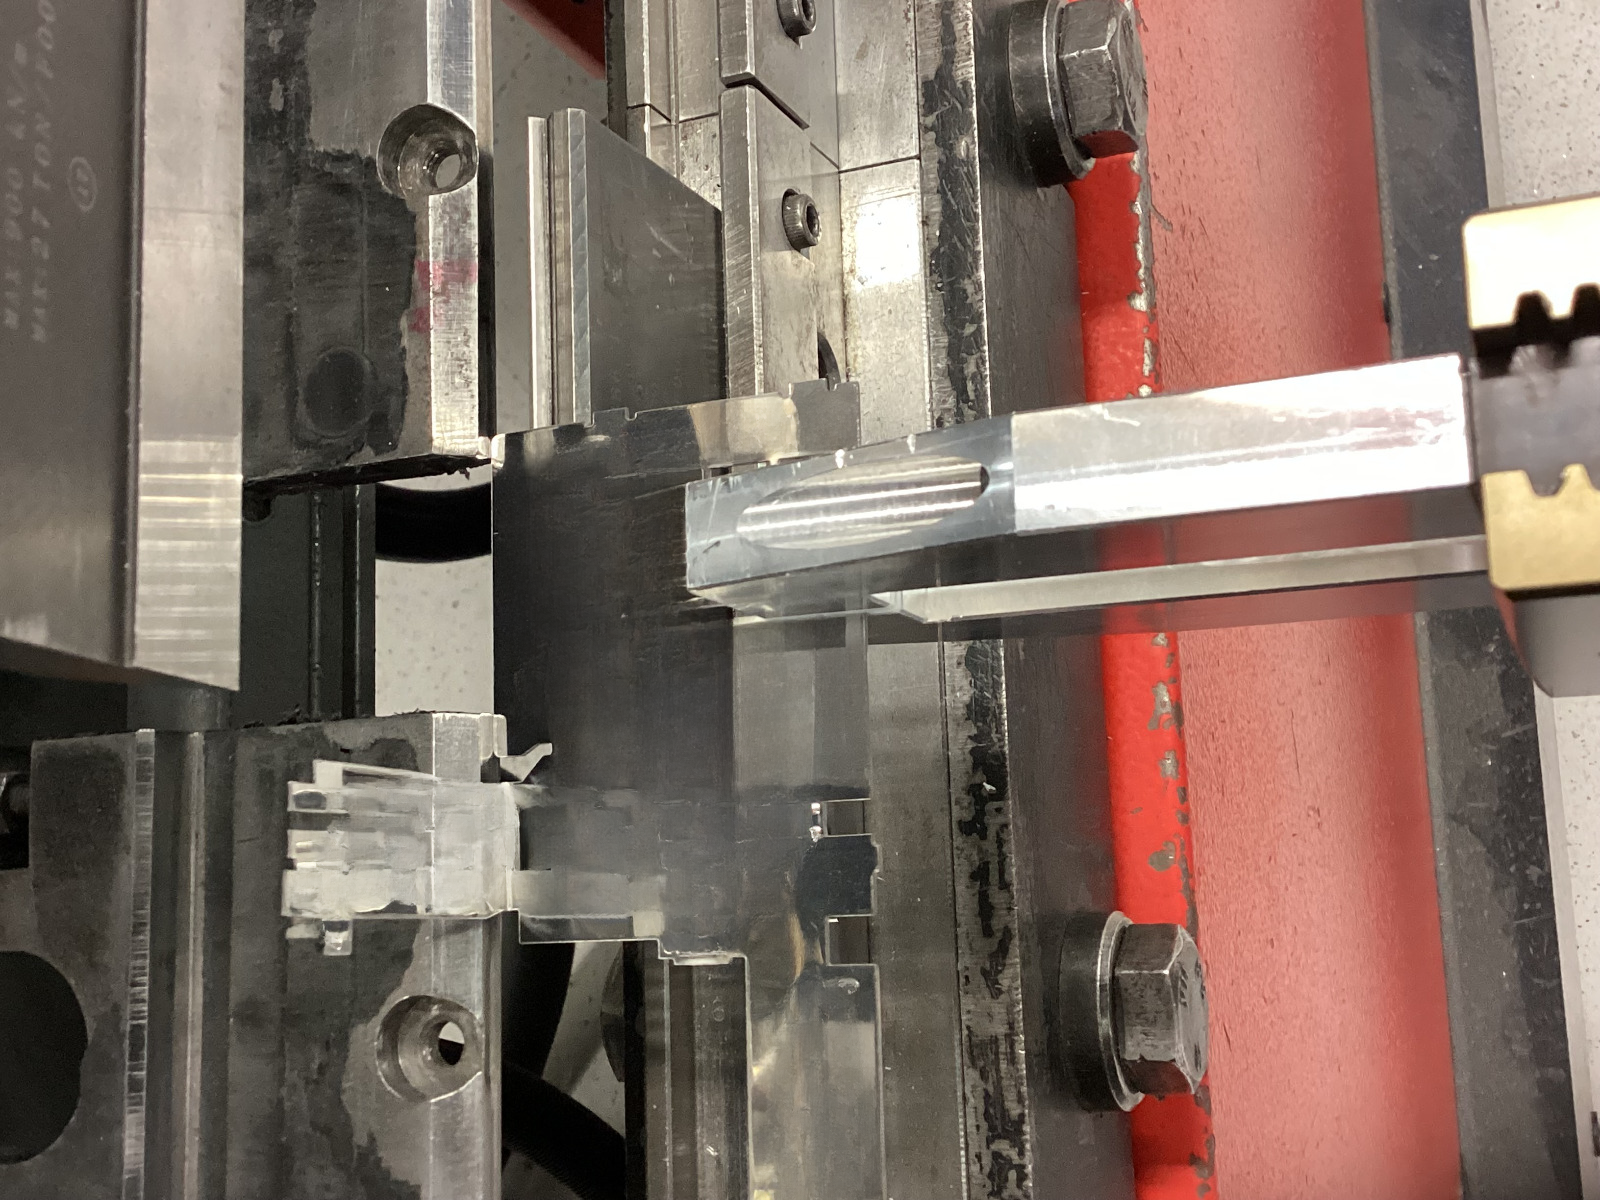
\includegraphics[width=\textwidth]{figures/bending/bending2-003.png}
        \caption{Go to bending station 2}
        \label{subfig:bending2-before}
    \end{subfigure}\hspace{0.1cm}
    \begin{subfigure}[b]{0.32\textwidth}
        \centering
        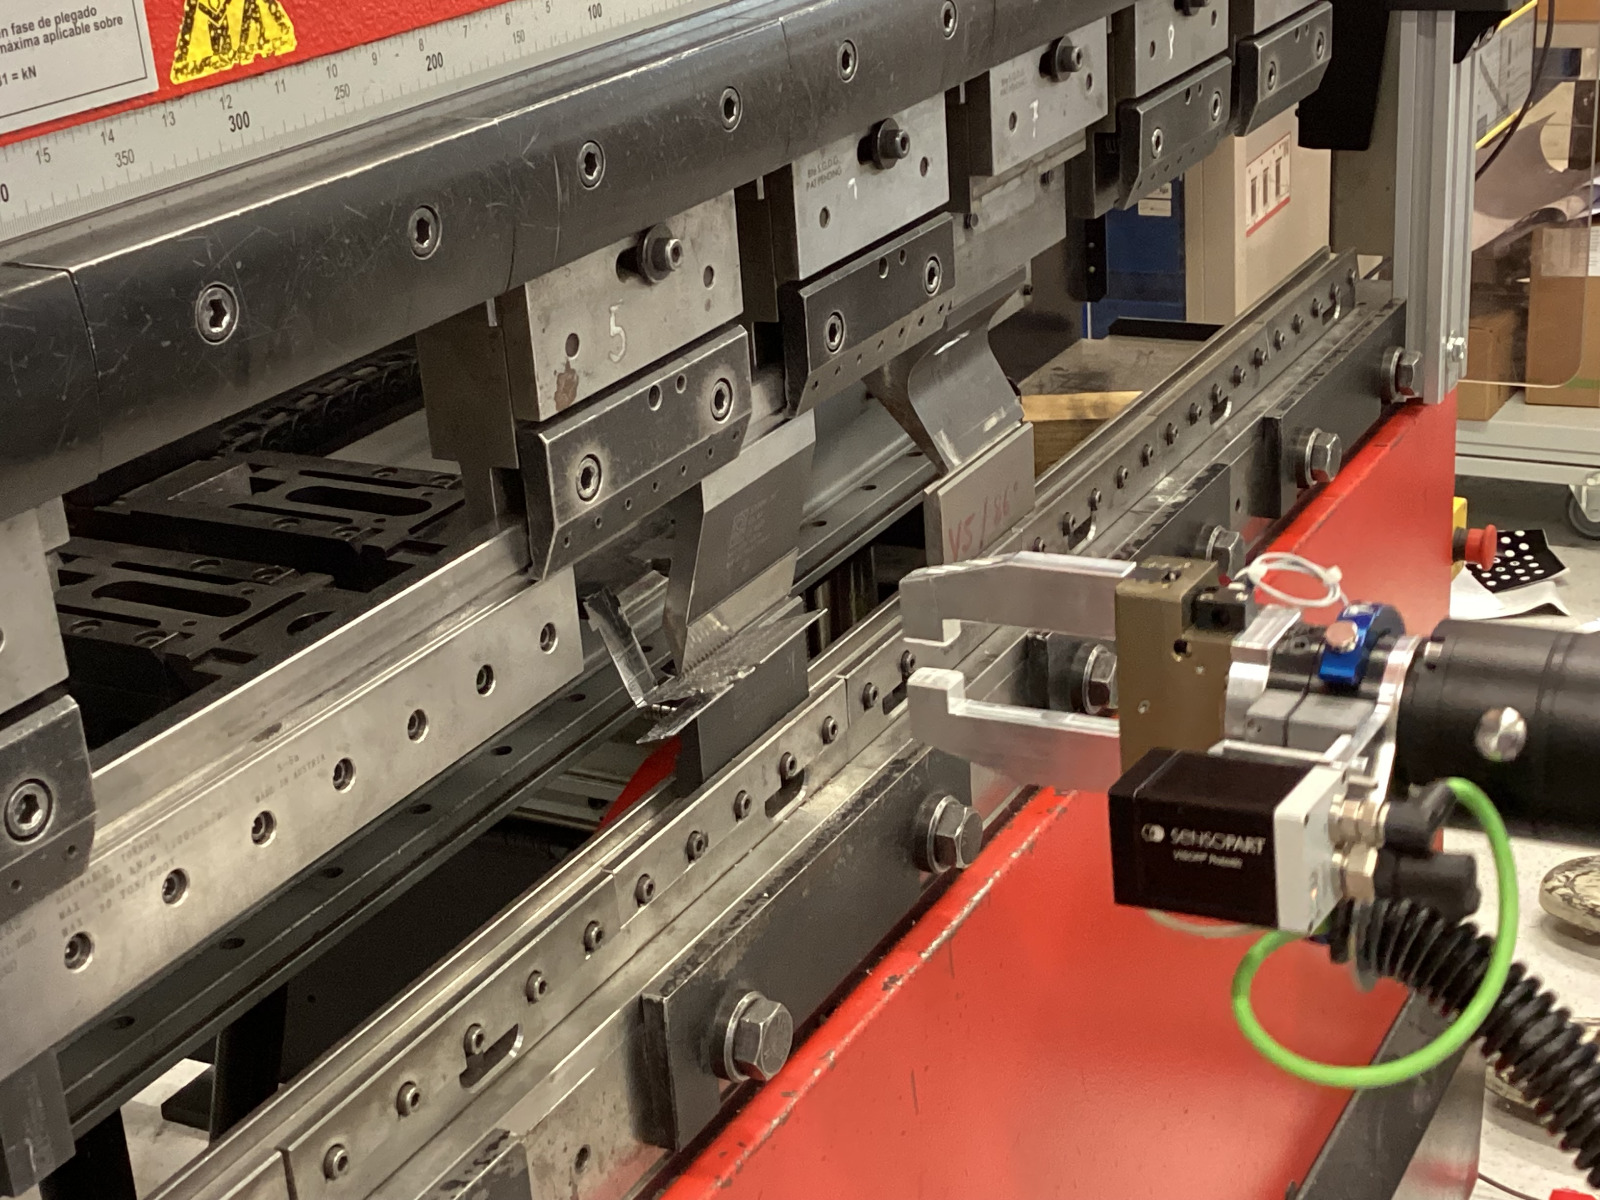
\includegraphics[width=\textwidth]{figures/bending/bending2-001.png}
        \caption{bend the sheet metal part}
        \label{subfig:bending2}
    \end{subfigure}\hspace{0.1cm}
    \begin{subfigure}[b]{0.32\textwidth}
        \centering
        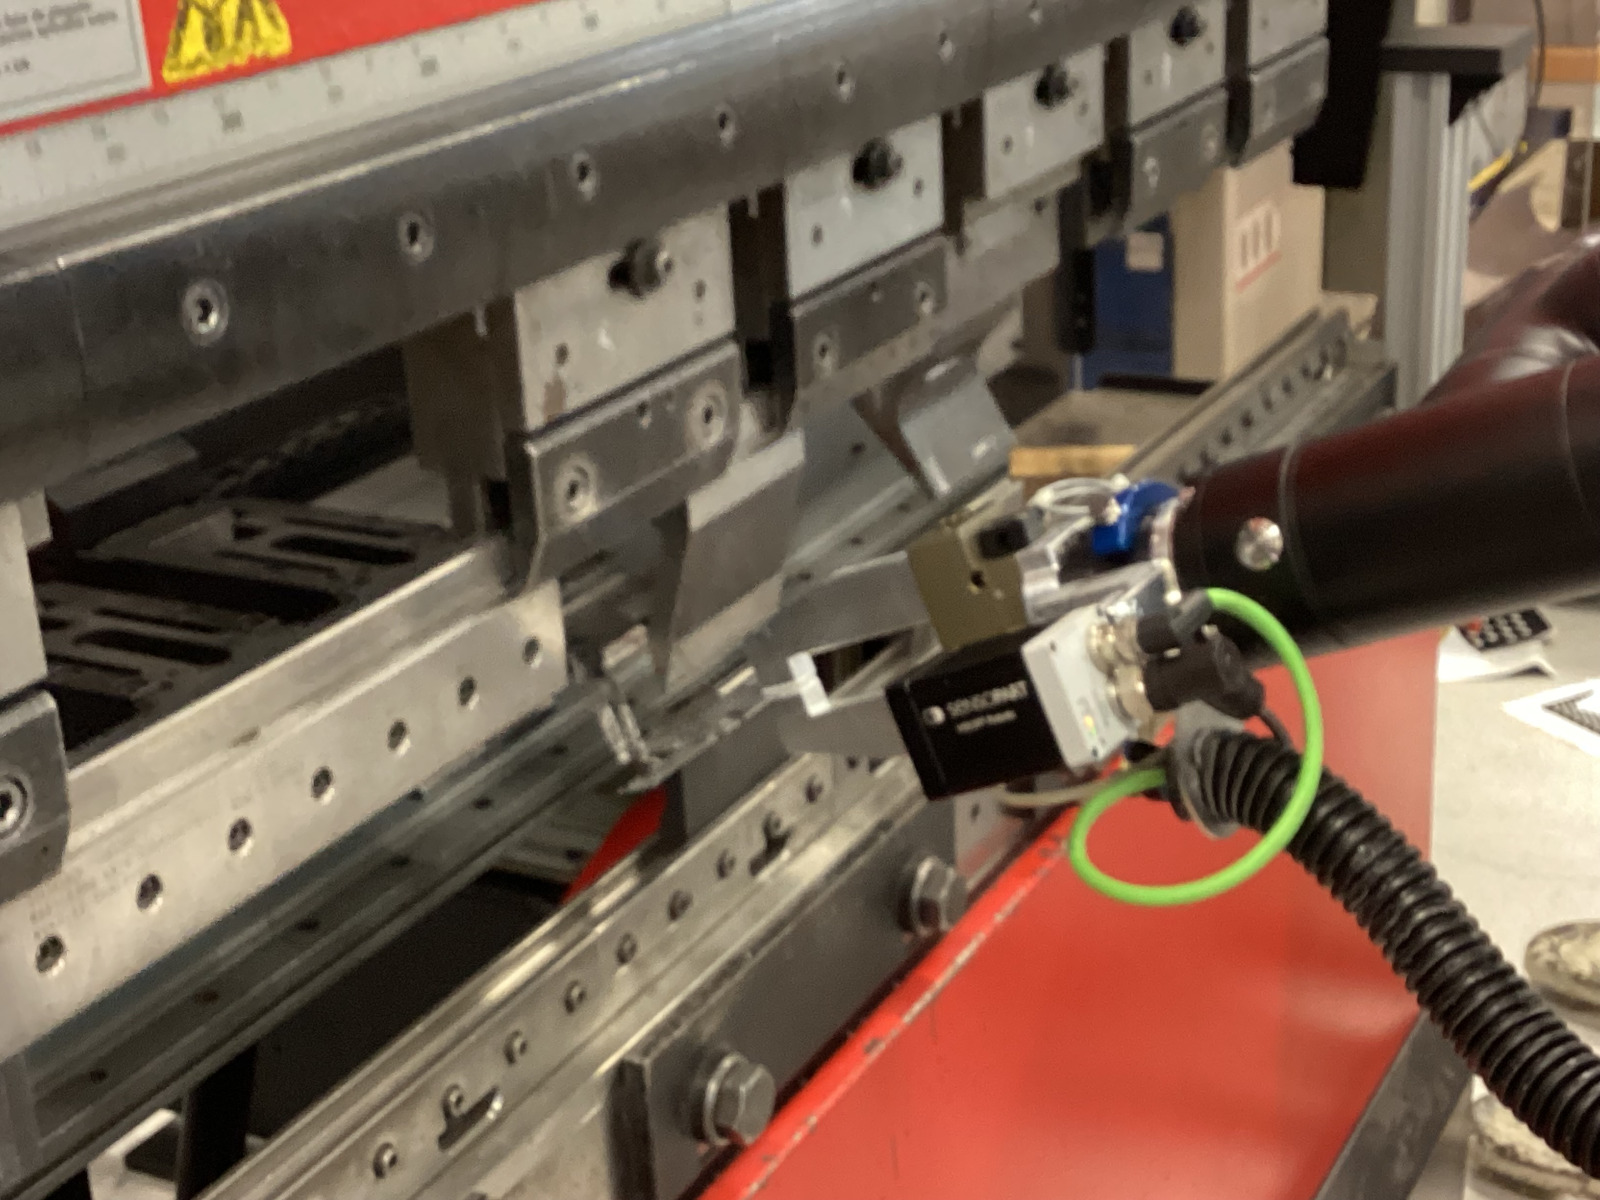
\includegraphics[width=\textwidth]{figures/bending/bending2-002.png}
        \caption{take away the bent sheet}
        \label{subfig:bending2-after}
    \end{subfigure}\hspace{0.1cm}
    \caption{Bending operation number 2 at bending station 2}
    \label{fig:bending-operation-2}
\end{figure}


Figure \ref{fig:bending-operation-1} shows the transfer of sheet metal part to the first bending station where a 90° bend is performed. The handling robot secures the sheet first. A signal is sent by KR1410 robot to PLC to start bending. The robot opens the gripper as soon as the tool of the bending machine hits the sheet. The sheet is secured by the bending machine and the robot moves to a different pose. From there, the robot moves back to the bent part and grip it. Another signal is sent to PLC to move the tool upwards. Once the tool is clear of the part, robot goes to the inspection camera for angle measurement. Bending machine open height measurement laser sensor is responsible for the timings of the opening and closing of bending machine signals. It helps in making robot work together with the bending machine and avoid any collision.


Figures \ref{fig:bending-operation-2} and \ref{fig:bending-operation-3} shows the bending of part at bending station 2. The process is similar to the first bending. The robot leaves the part during bending and regrip it once the bending is complete. For bending number 3, an inspection is not done, because the bending is done very close to the edge, and the small edge is not measurable by the inspection camera.


\begin{figure}[h]
    \centering
    \begin{subfigure}[b]{0.32\textwidth}
        \centering
        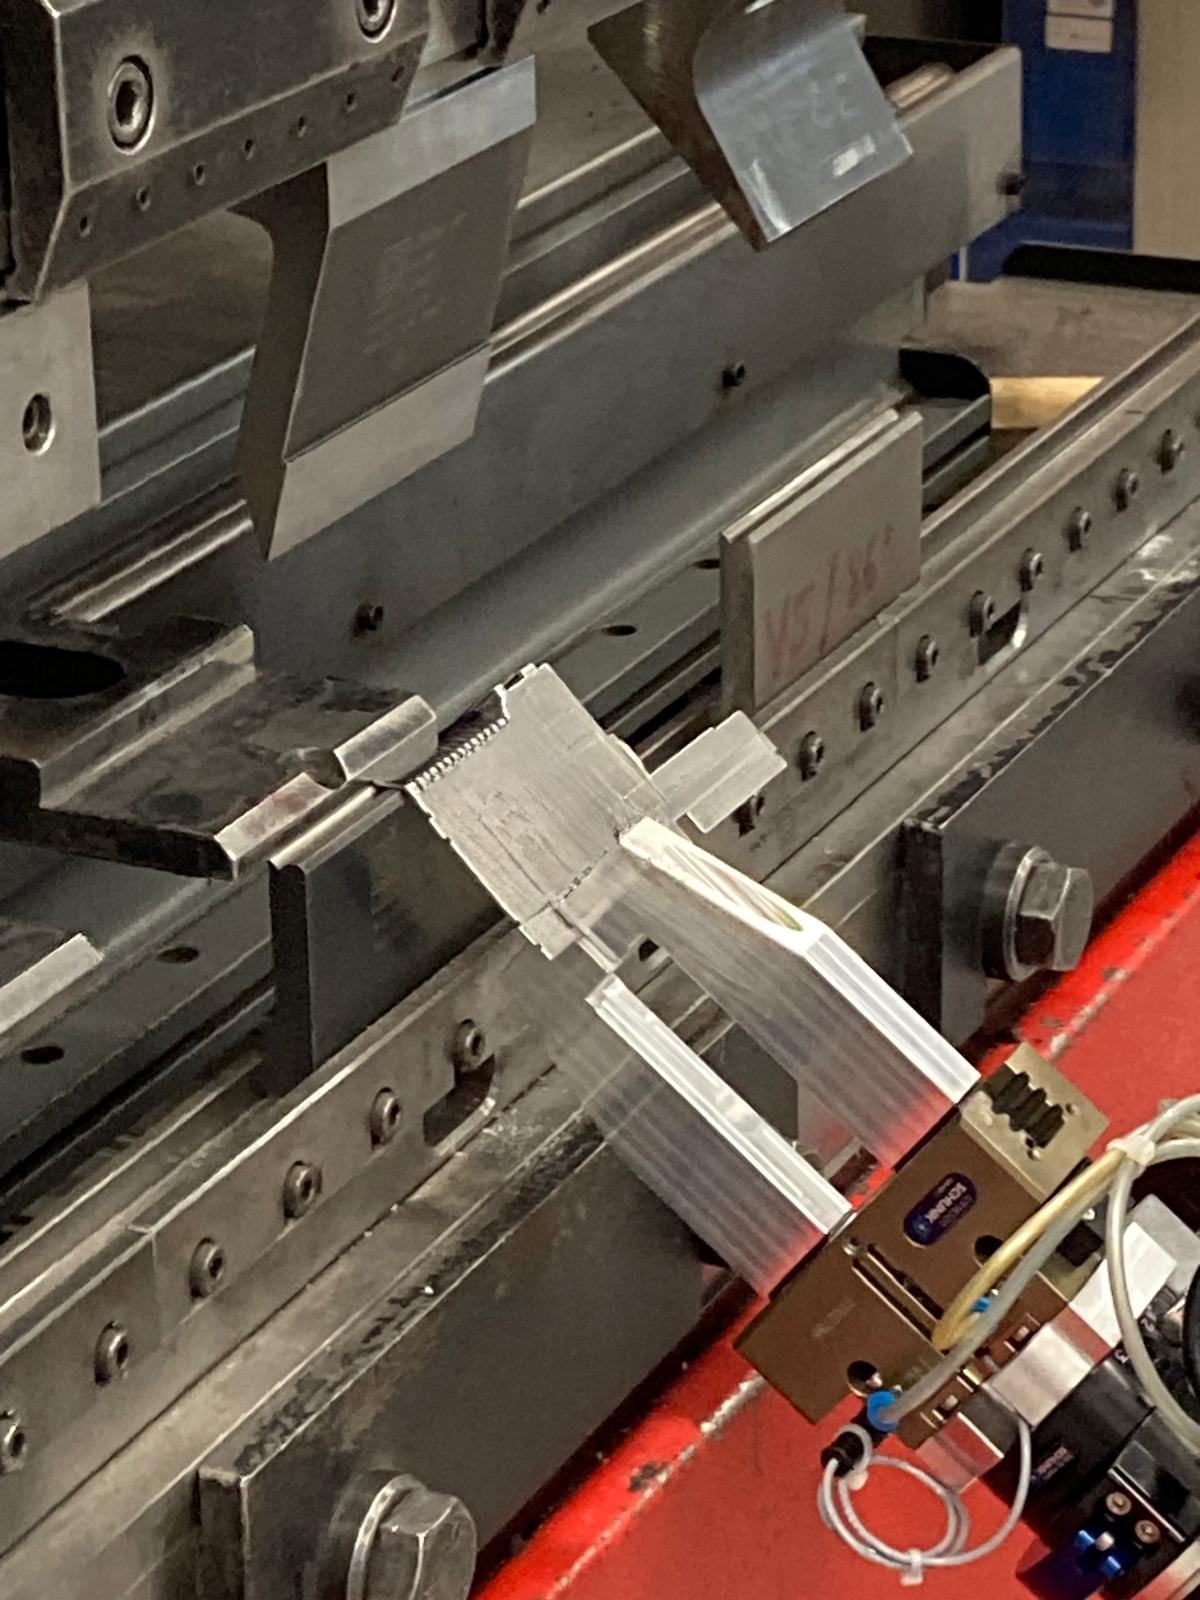
\includegraphics[width=\textwidth]{figures/bending/bending3-001.png}
        \caption{Go to bending station 2}
        \label{subfig:bending3-before}
    \end{subfigure}\hspace{0.1cm}
    \begin{subfigure}[b]{0.32\textwidth}
        \centering
        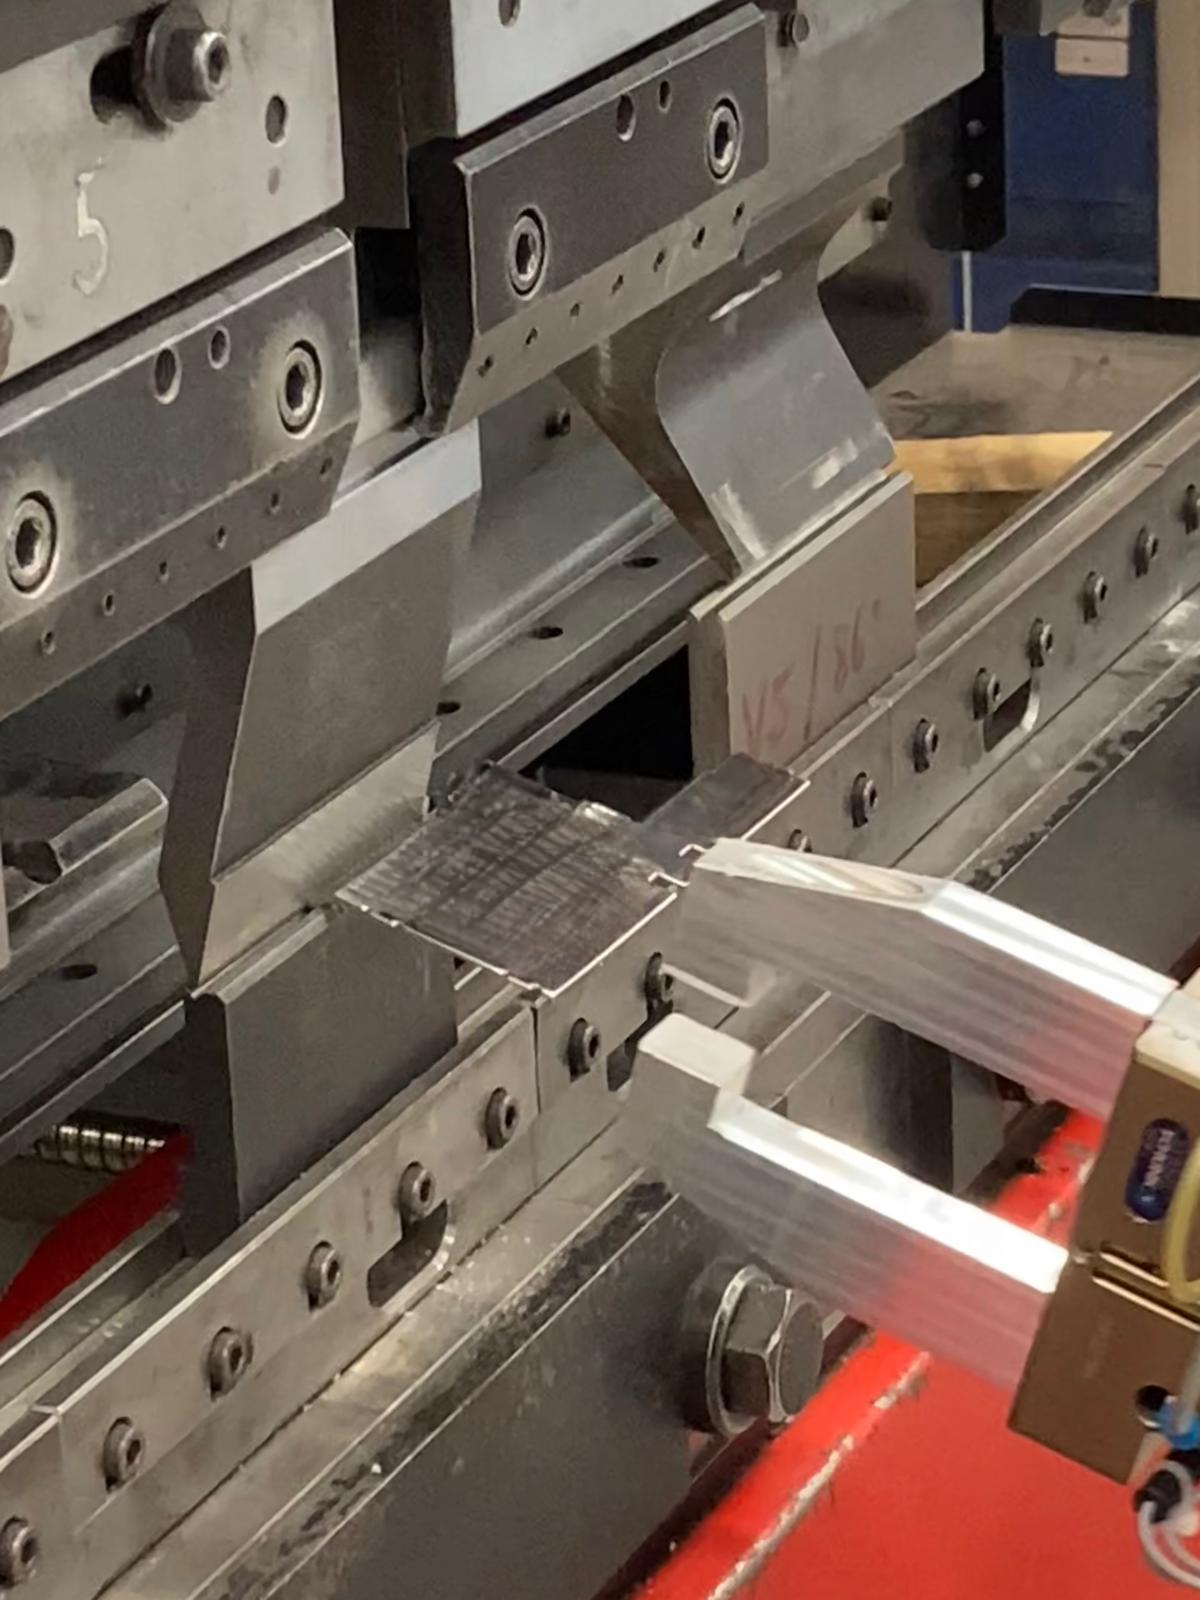
\includegraphics[width=\textwidth]{figures/bending/bending3-002.png}
        \caption{bend the sheet metal part}
        \label{subfig:bending3}
    \end{subfigure}\hspace{0.1cm}
    \begin{subfigure}[b]{0.32\textwidth}
        \centering
        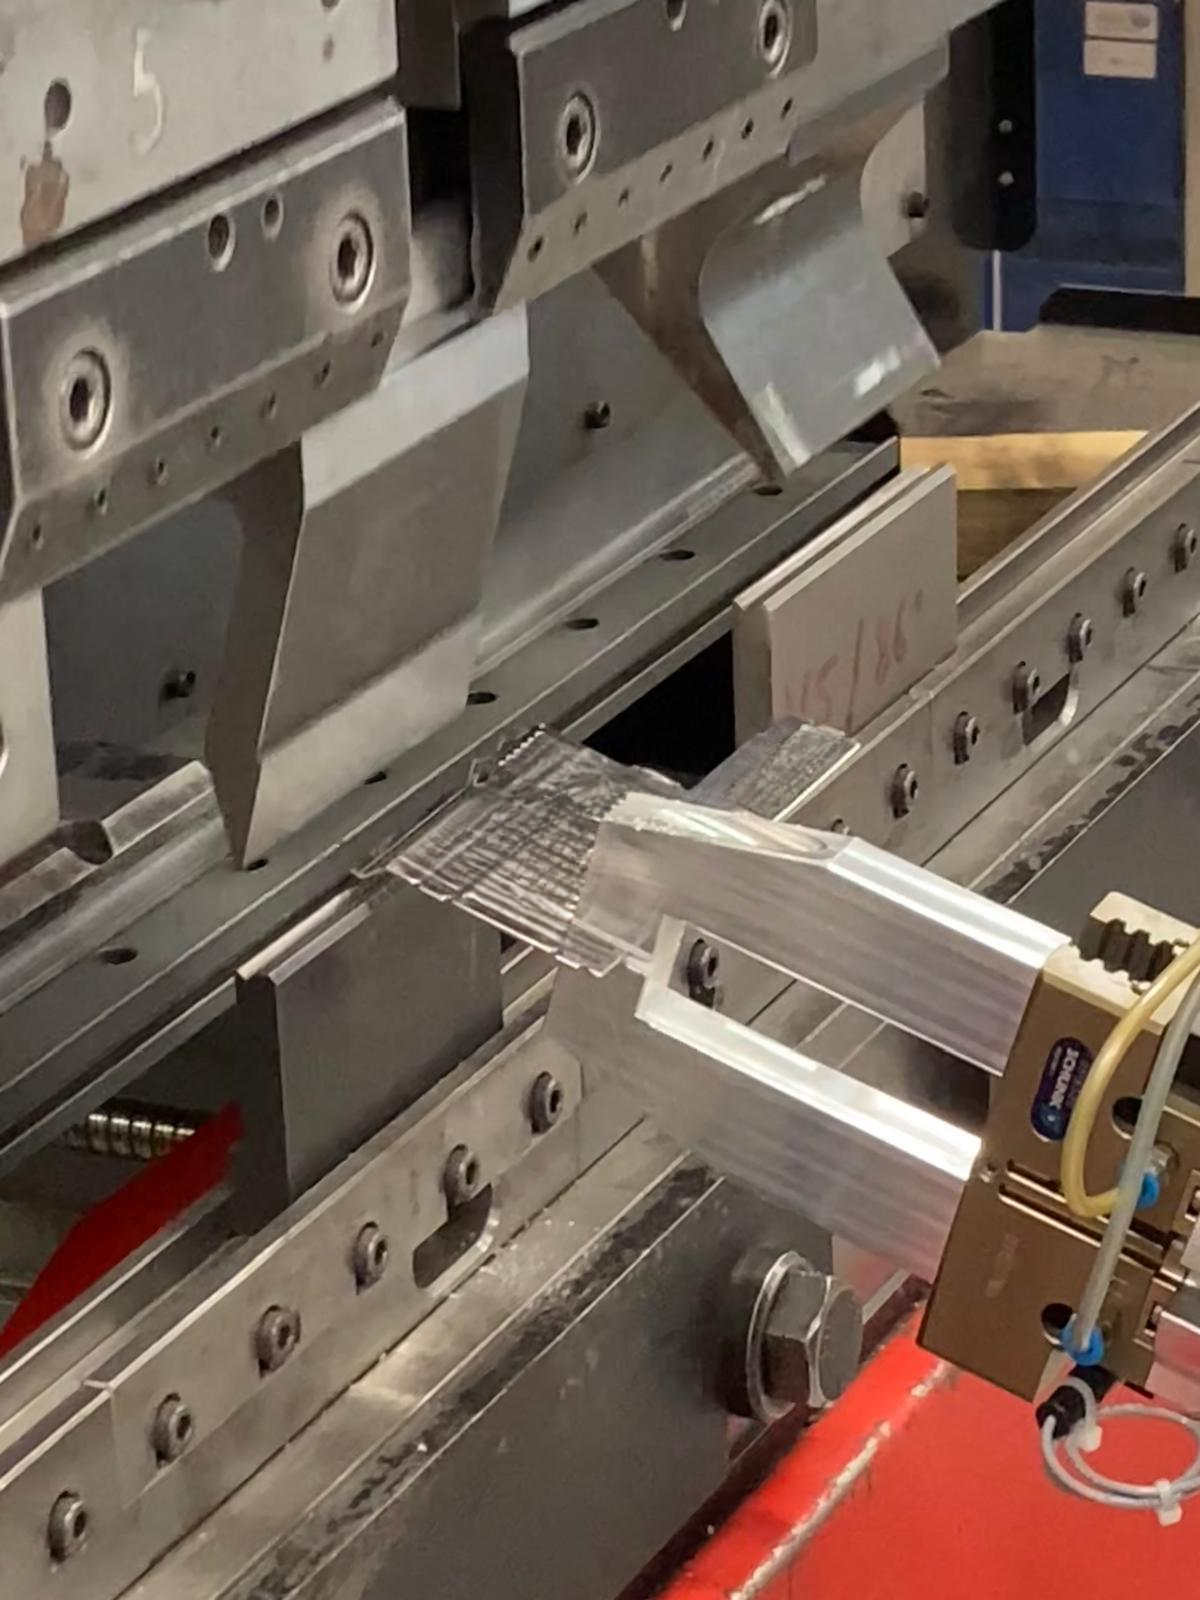
\includegraphics[width=\textwidth]{figures/bending/bending3-003.png}
        \caption{take away the bent sheet}
        \label{subfig:bending3-after}
    \end{subfigure}\hspace{0.1cm}
    \caption{Bending operation number 3 at bending station 2}
    \label{fig:bending-operation-3}
\end{figure}

\begin{figure}[h]
    \centering
    \begin{subfigure}[b]{0.32\textwidth}
        \centering
        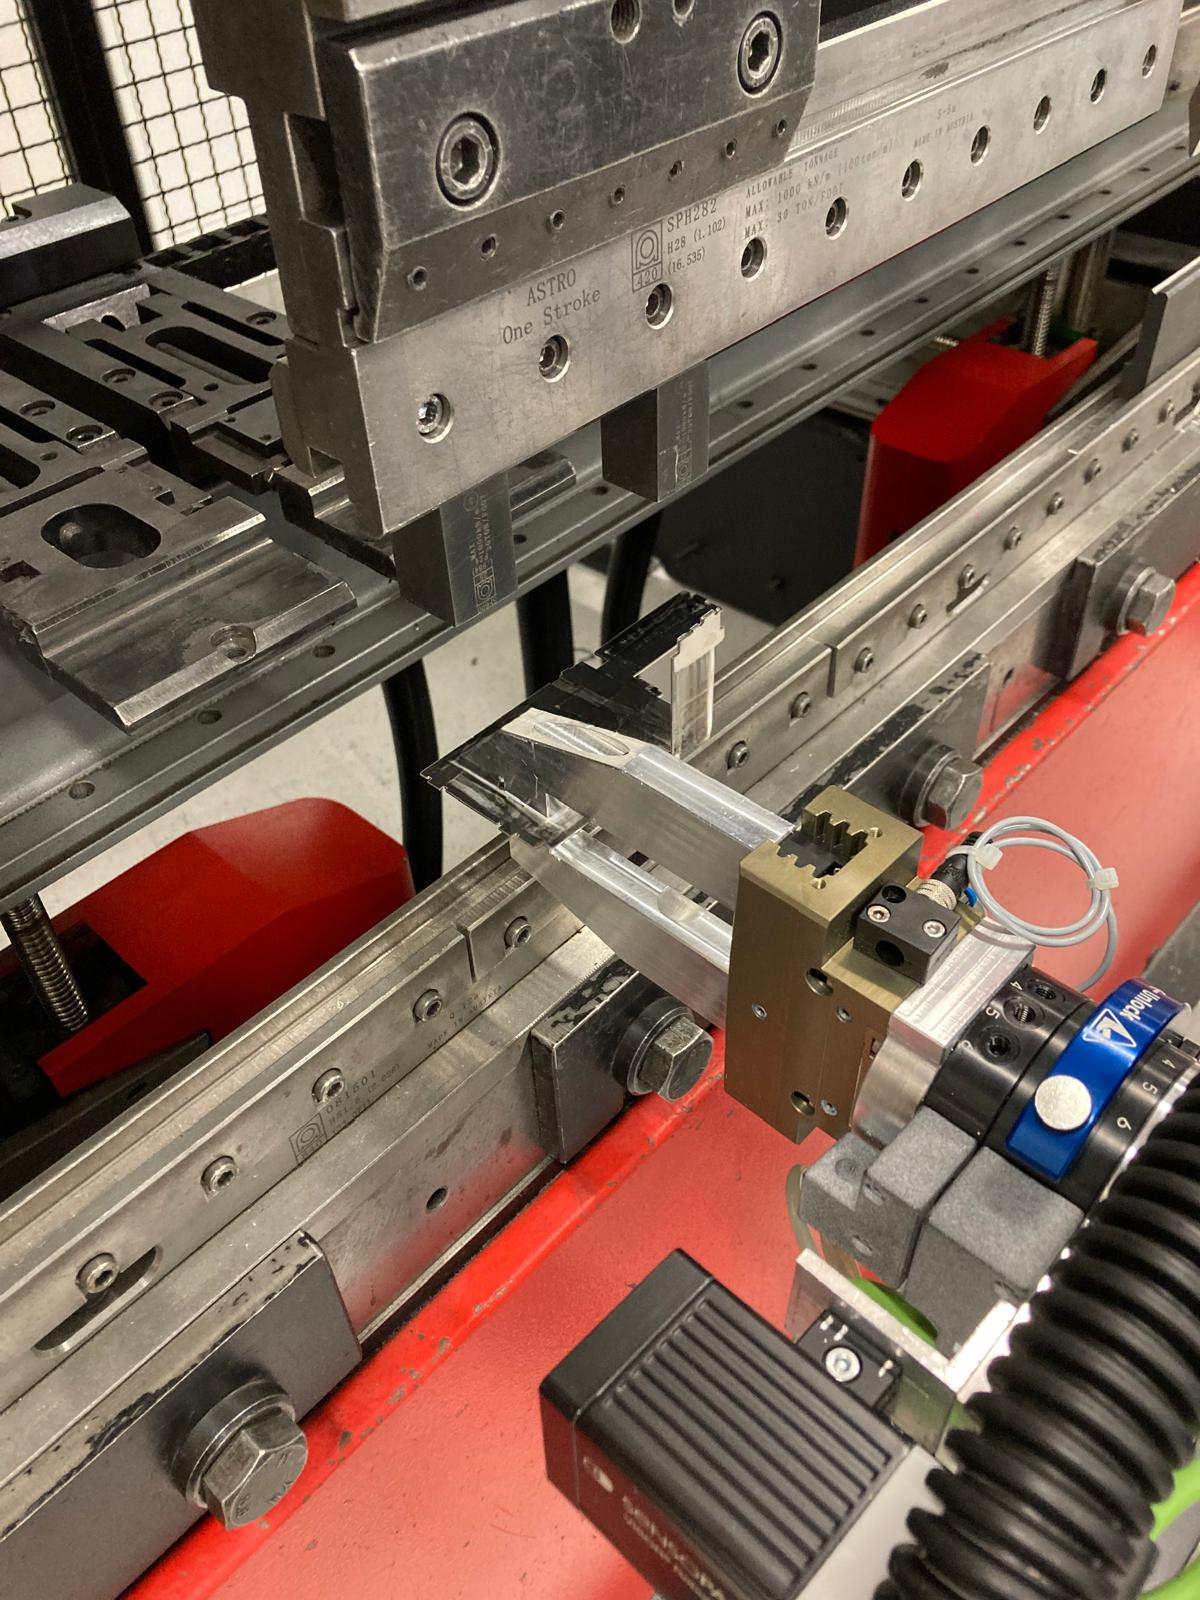
\includegraphics[width=\textwidth]{figures/bending/bending4-001.png}
        \caption{Go to bending station 3}
        \label{subfig:bending4-before}
    \end{subfigure}\hspace{0.1cm}
    \begin{subfigure}[b]{0.32\textwidth}
        \centering
        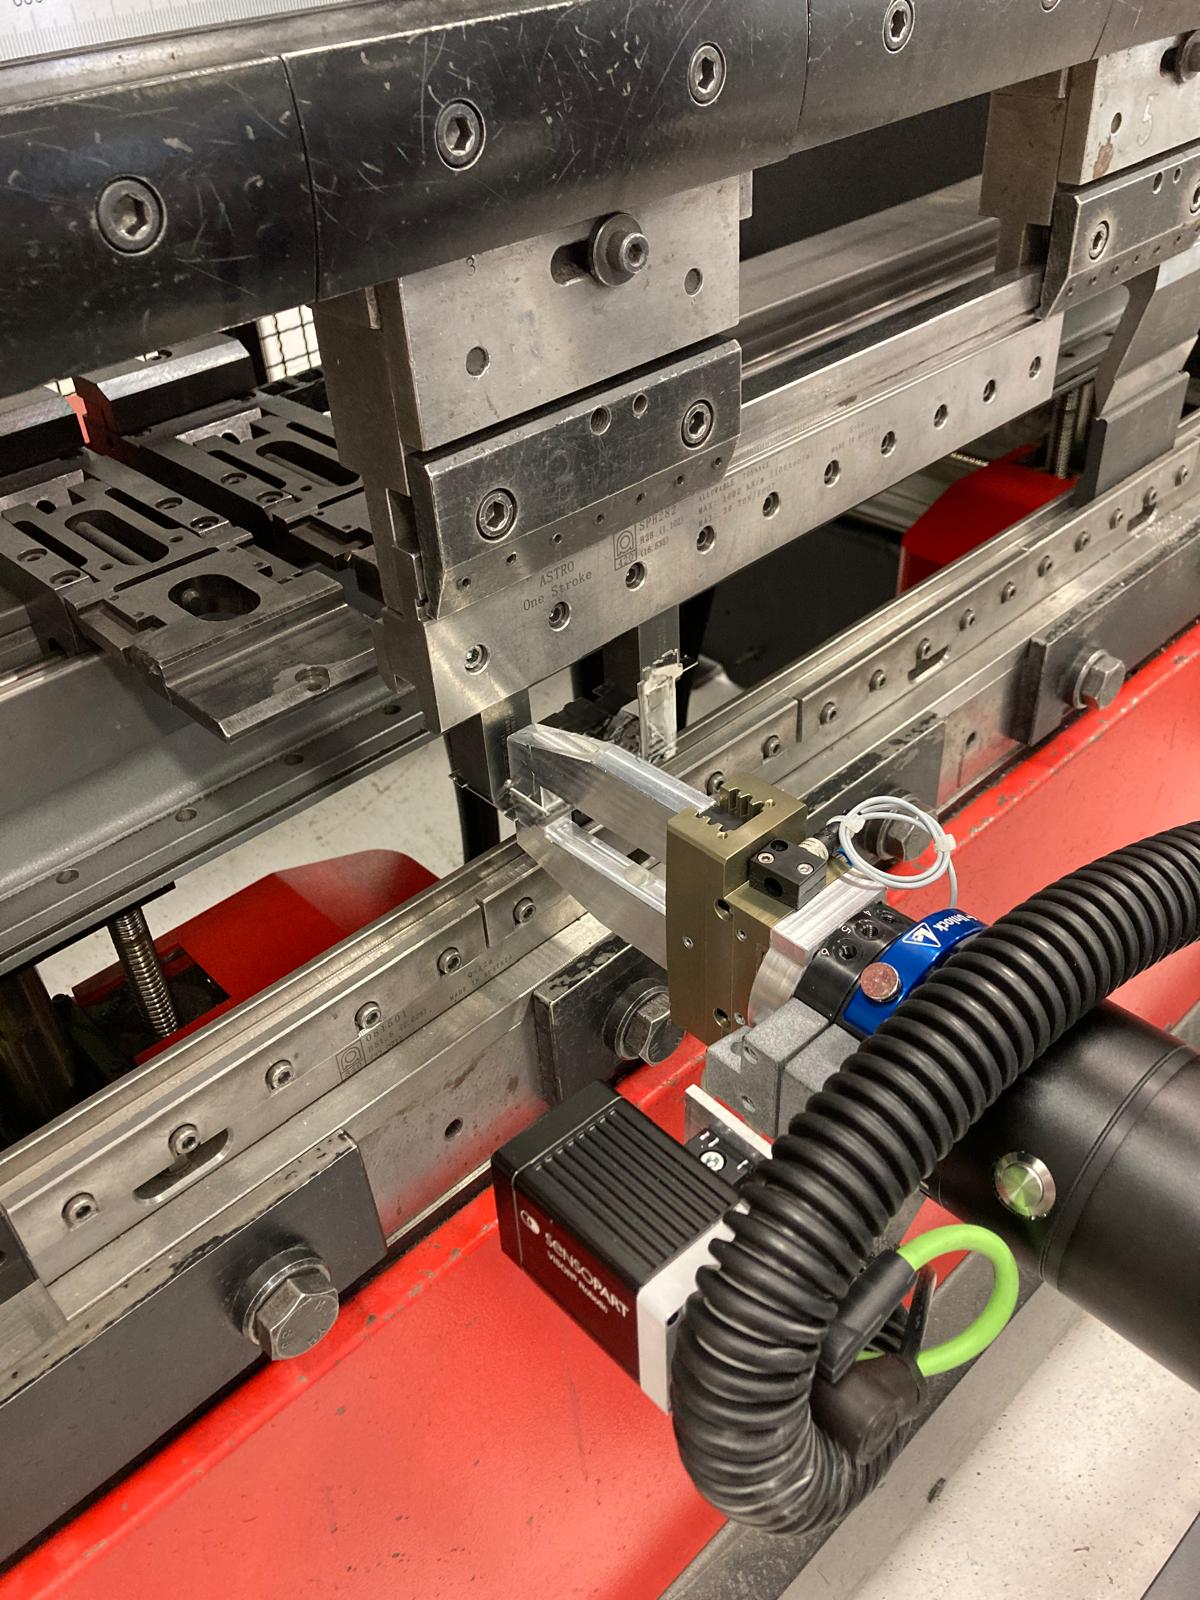
\includegraphics[width=\textwidth]{figures/bending/bending4-002.png}
        \caption{bend the sheet metal part}
        \label{subfig:bending4}
    \end{subfigure}\hspace{0.1cm}
    \begin{subfigure}[b]{0.32\textwidth}
        \centering
        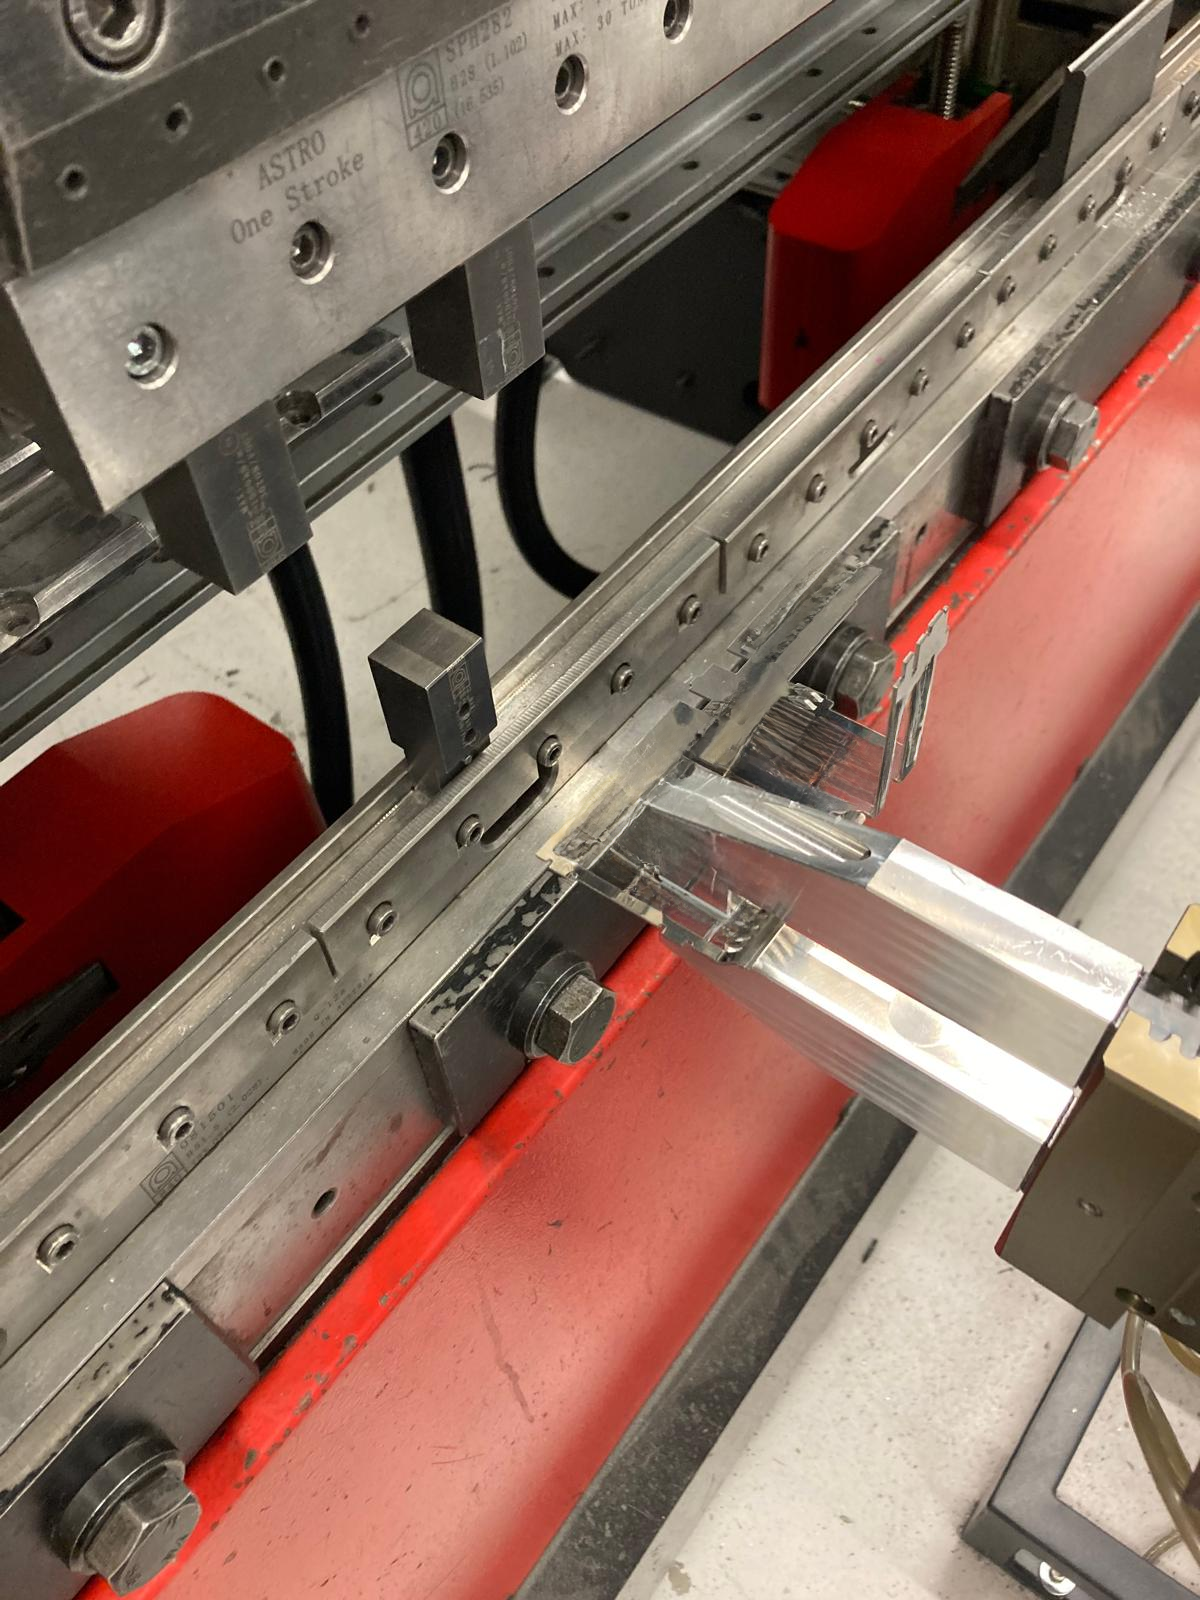
\includegraphics[width=\textwidth]{figures/bending/bending4-003.png}
        \caption{take away the bent sheet}
        \label{subfig:bending4-after}
    \end{subfigure}\hspace{0.1cm}
    \caption{Bending operation number 4 at bending station 3}
    \label{fig:bending-operation-4}
\end{figure}


Figure \ref{fig:bending-operation-4} shows the bending opertion number 4. Since the tool and die are only used for pressing the sheet to flatten it, the robotic gripper doesn't have to open the gripper during bending. Once the sheet is pressed for a specific duration, tool moves up and the robot takes the part out.  Again the inspection is not done, because there is no warping of sheet in this bending operation.


\begin{figure}[h]
    \centering
    \begin{subfigure}[b]{0.32\textwidth}
        \centering
        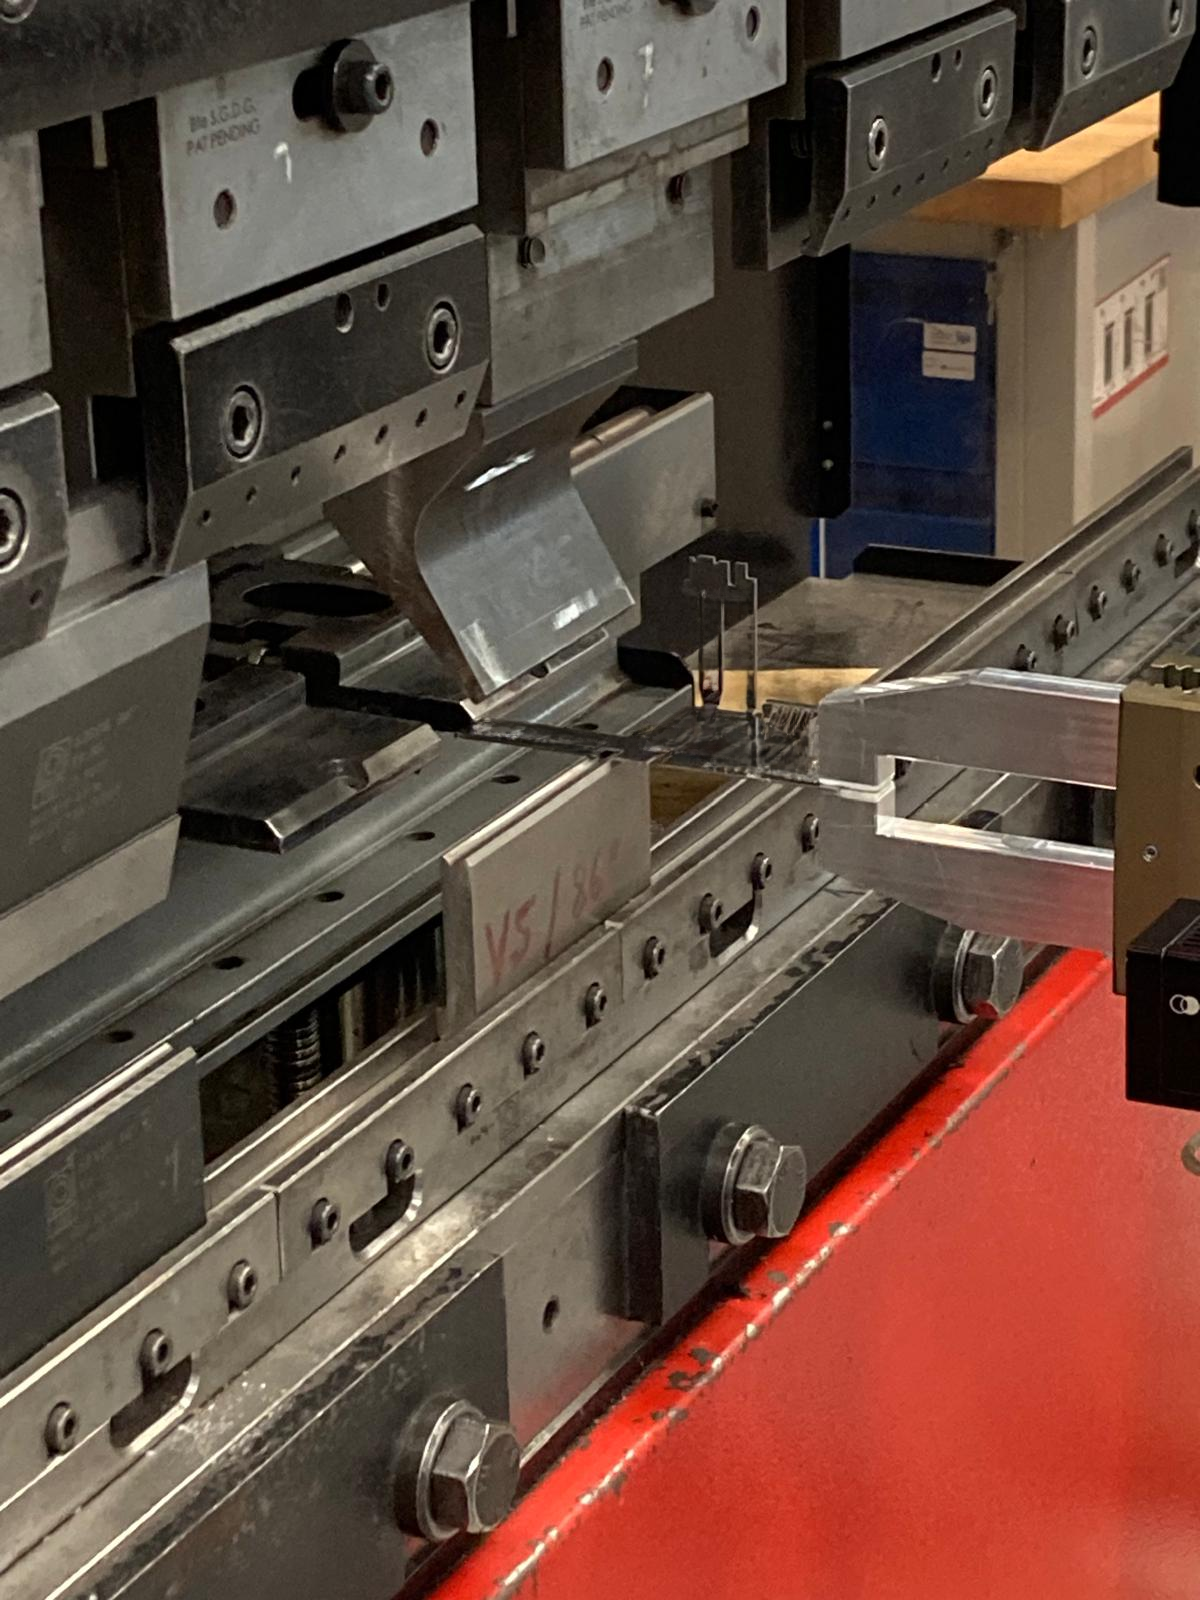
\includegraphics[width=\textwidth]{figures/bending/bending5-001.png}
        \caption{Go to bending station 1}
        \label{subfig:bending5-before}
    \end{subfigure}\hspace{0.1cm}
    \begin{subfigure}[b]{0.32\textwidth}
        \centering
        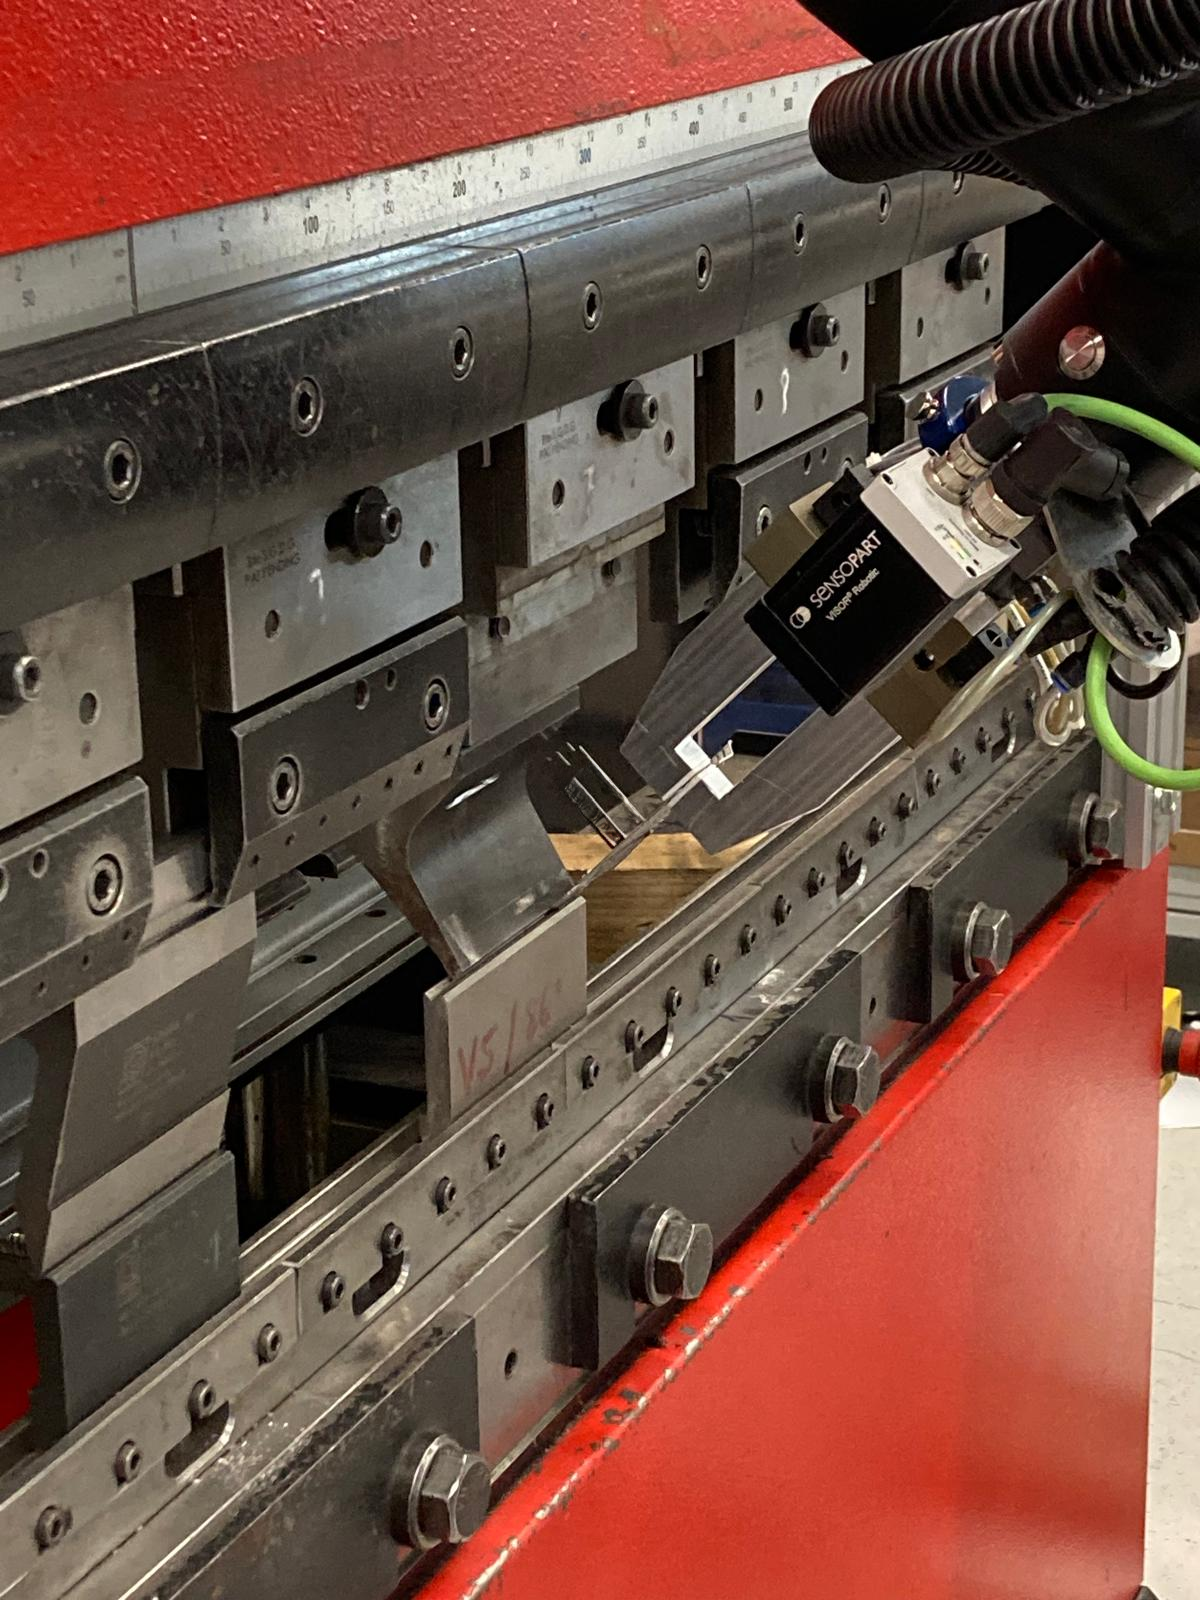
\includegraphics[width=\textwidth]{figures/bending/bending5-002.png}
        \caption{bend the sheet metal part}
        \label{subfig:bending5}
    \end{subfigure}\hspace{0.1cm}
    \begin{subfigure}[b]{0.32\textwidth}
        \centering
        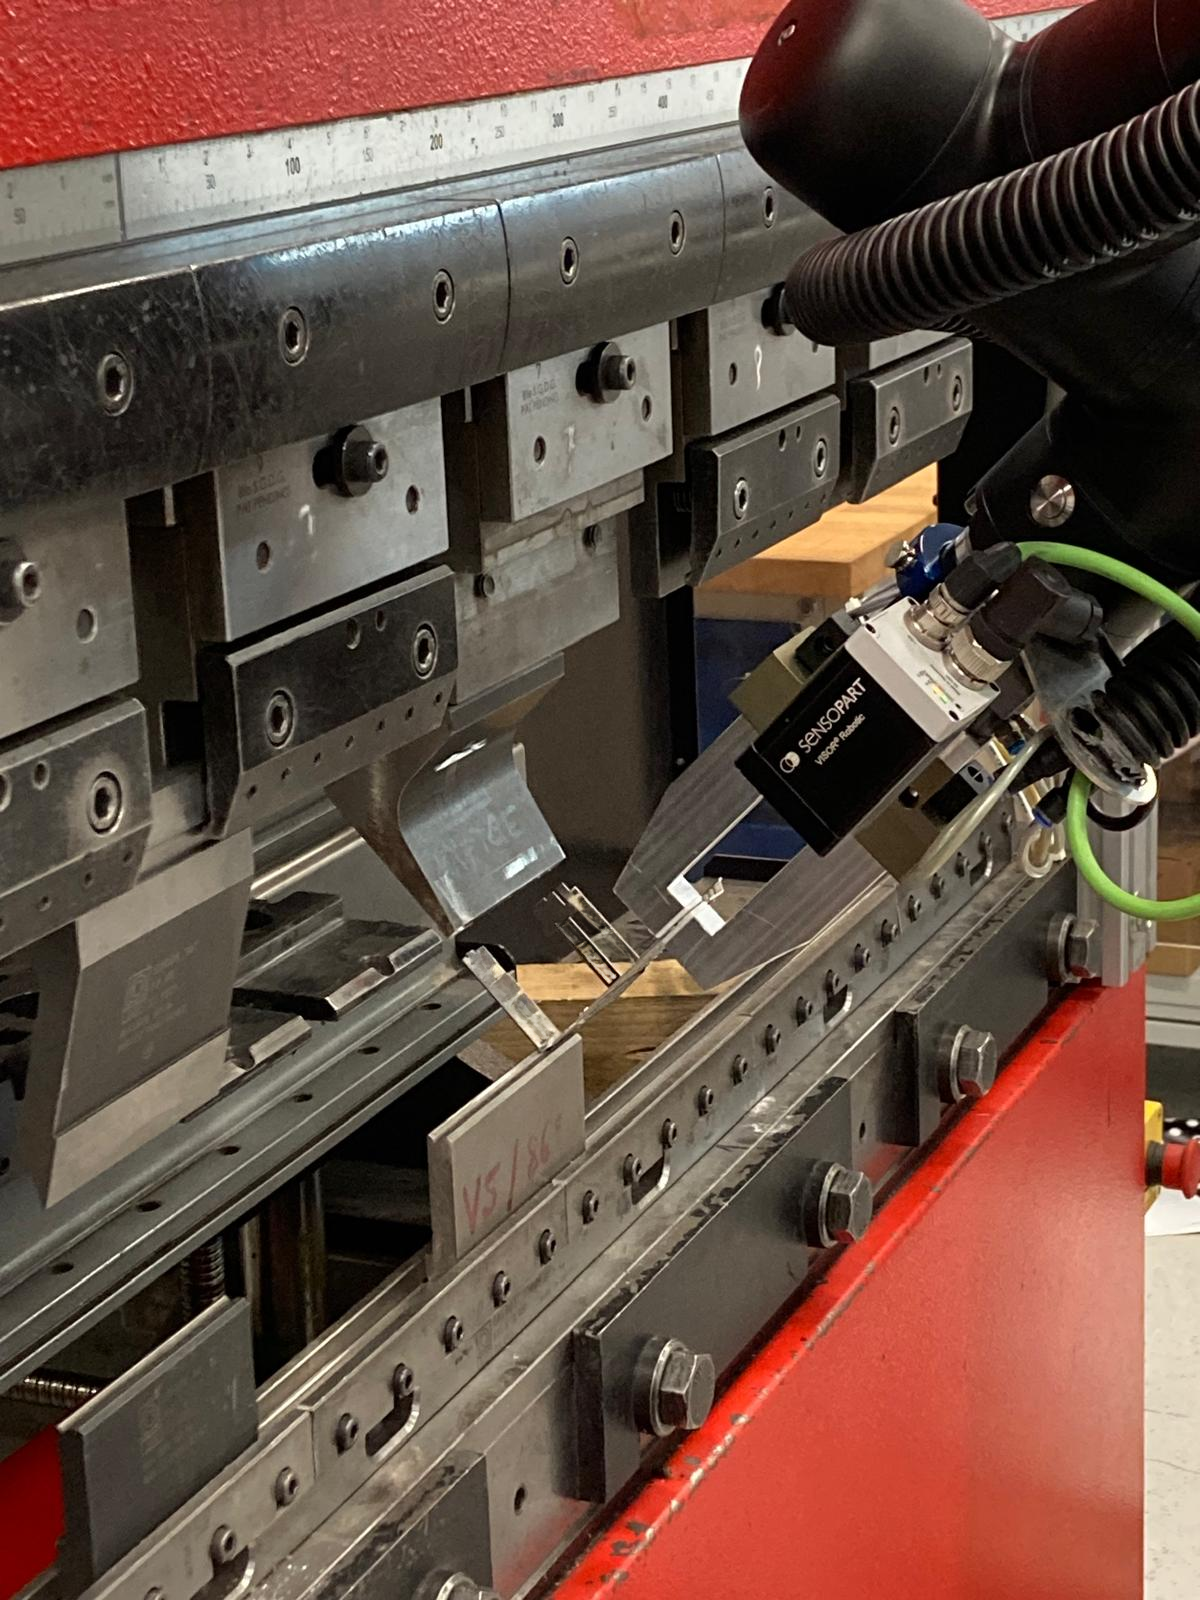
\includegraphics[width=\textwidth]{figures/bending/bending5-003.png}
        \caption{take away the bent sheet}
        \label{subfig:bending5-after}
    \end{subfigure}\hspace{0.1cm}
    \caption{Bending operation number 5 at bending station 1}
    \label{fig:bending-operation-5}
\end{figure}


\begin{figure}[h]
    \centering
    \begin{subfigure}[b]{0.32\textwidth}
        \centering
        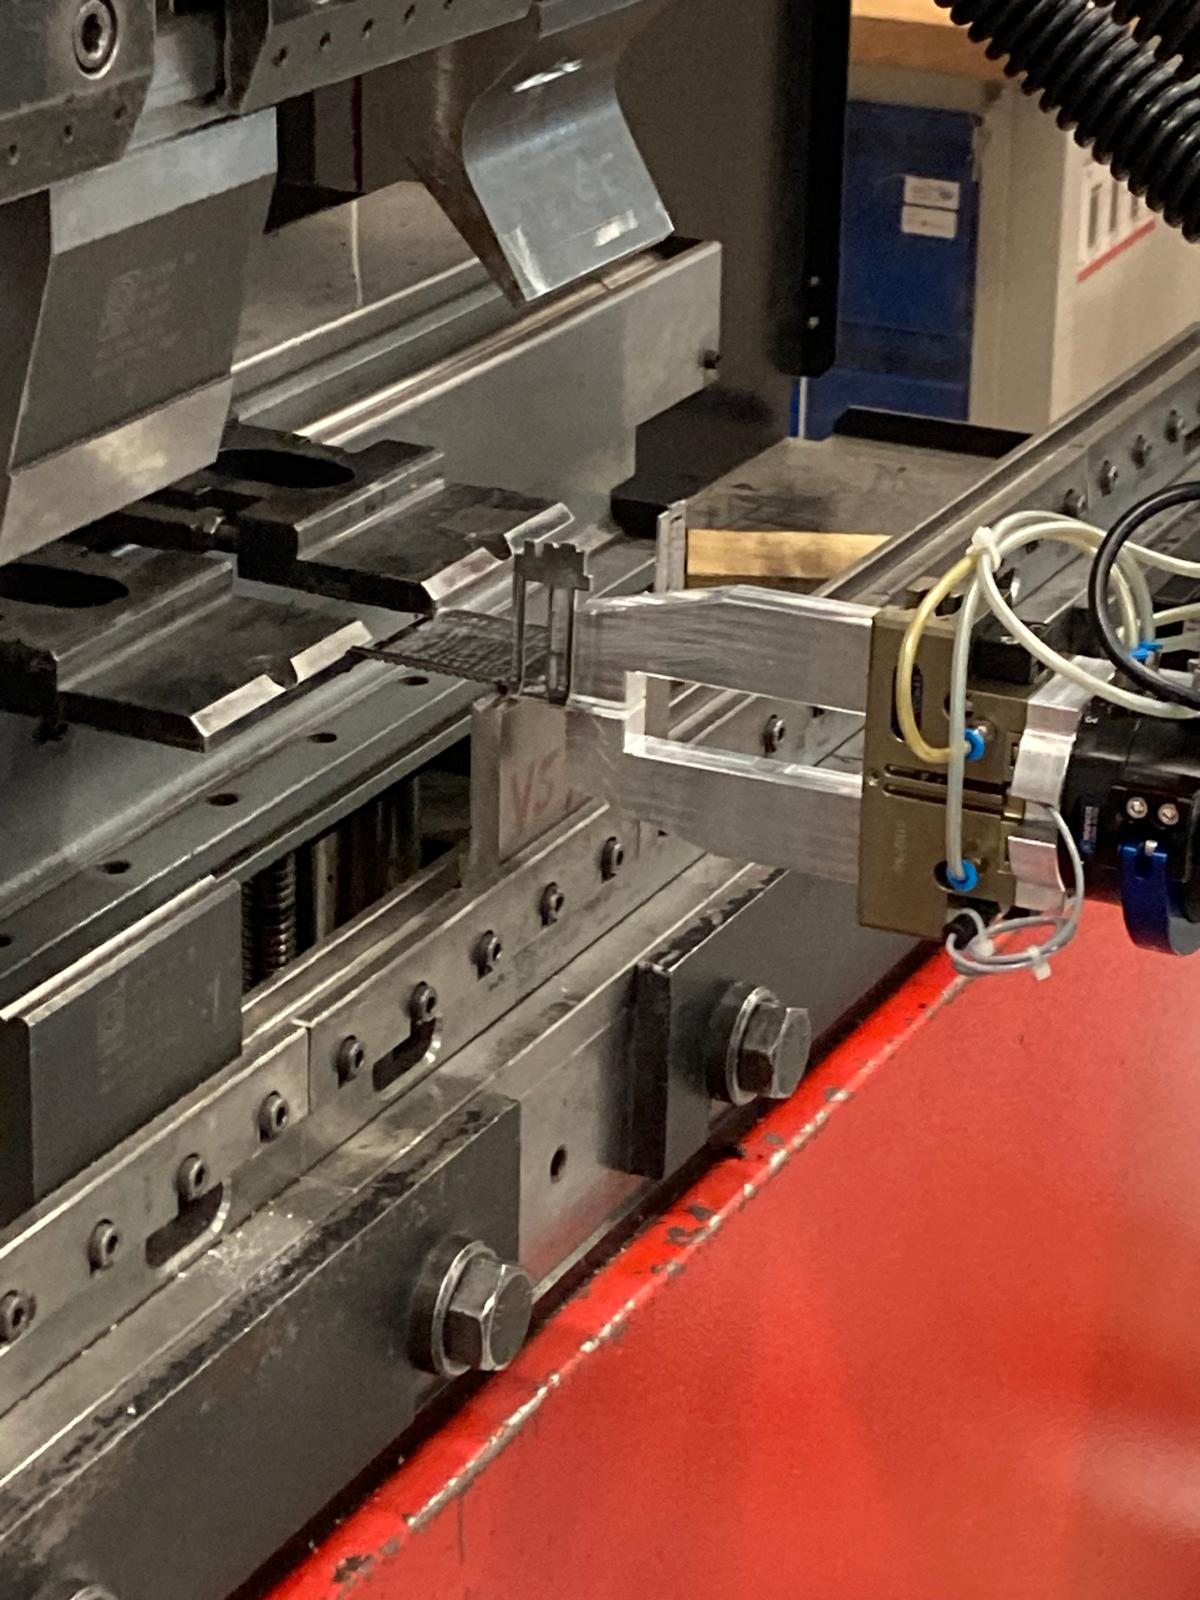
\includegraphics[width=\textwidth]{figures/bending/bending6-001.png}
        \caption{Go to bending station 1}
        \label{subfig:bending6-before}
    \end{subfigure}\hspace{0.1cm}
    \begin{subfigure}[b]{0.32\textwidth}
        \centering
        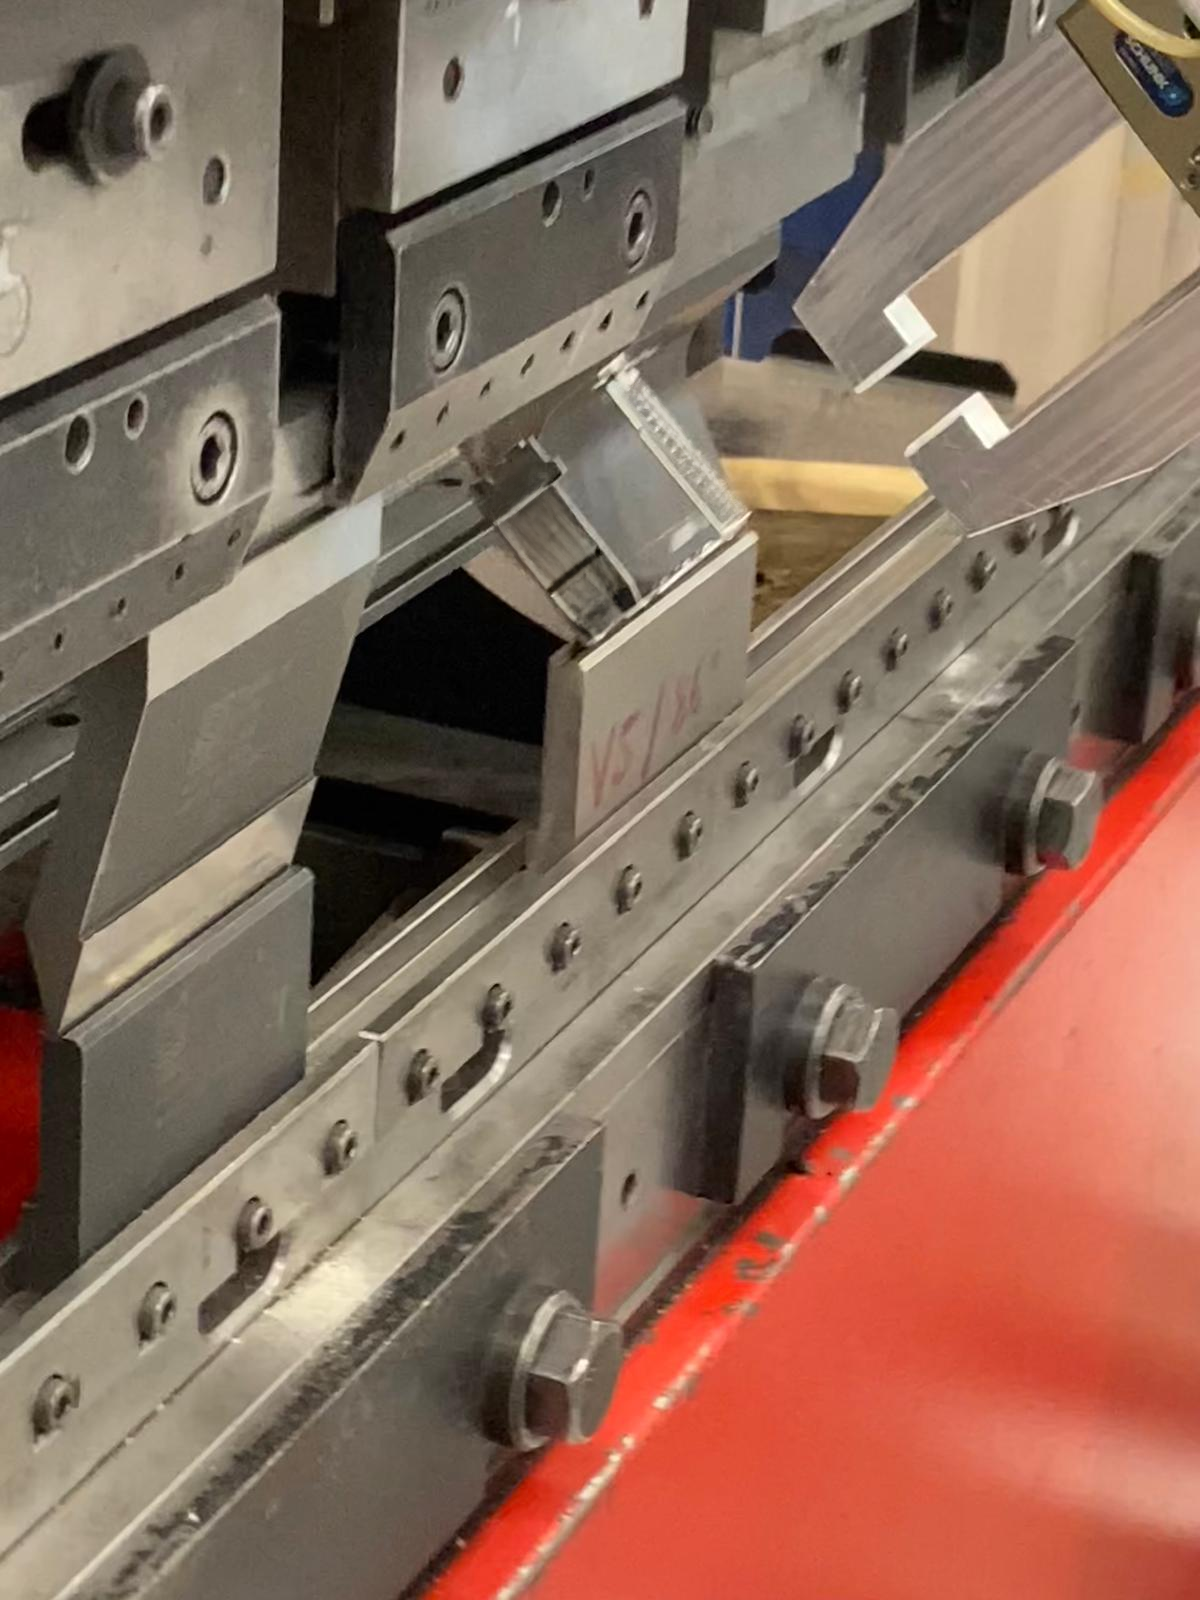
\includegraphics[width=\textwidth]{figures/bending/bending6-003.png}
        \caption{bend the sheet metal part}
        \label{subfig:bending6}
    \end{subfigure}\hspace{0.1cm}
    \begin{subfigure}[b]{0.32\textwidth}
        \centering
        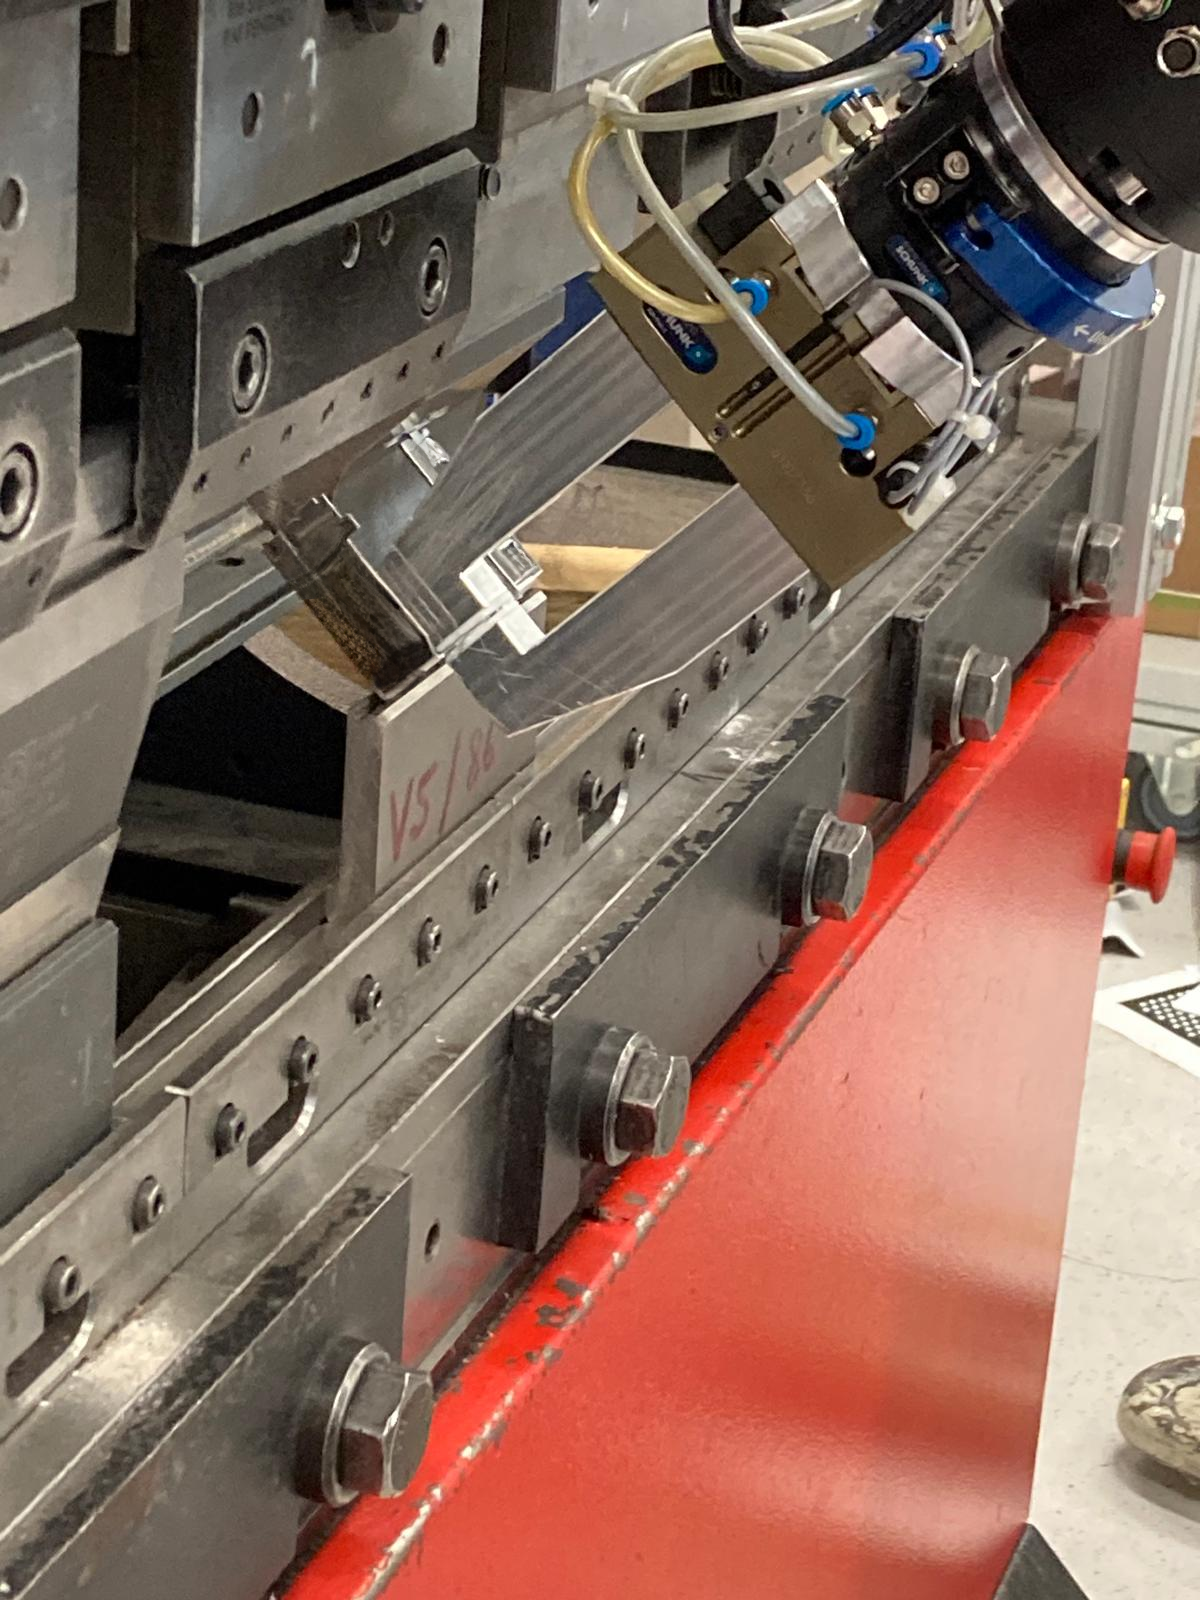
\includegraphics[width=\textwidth]{figures/bending/bending6-002.png}
        \caption{take away the bent sheet}
        \label{subfig:bending6-after}
    \end{subfigure}\hspace{0.1cm}
    \caption{Bending operation number 6 at bending station 1}
    \label{fig:bending-operation-6}
\end{figure}

Bending operation 5 and 6 are performed at bending station 1 as showing in figures \ref{fig:bending-operation-5} and \ref{fig:bending-operation-6} respectively. The process is similar to bending operation 1 as the robot doesn't hold the part during bending. Inspection is done after both bending operations. If after bending operation 6, the angle measurement is within tolerances, the current bending cycle is termed as successful.

\subsection{Shelf Control}
\label{subsec:shelf-control}

\begin{figure}[h]
    \centering
    \begin{subfigure}[b]{0.32\textwidth}
        \centering
        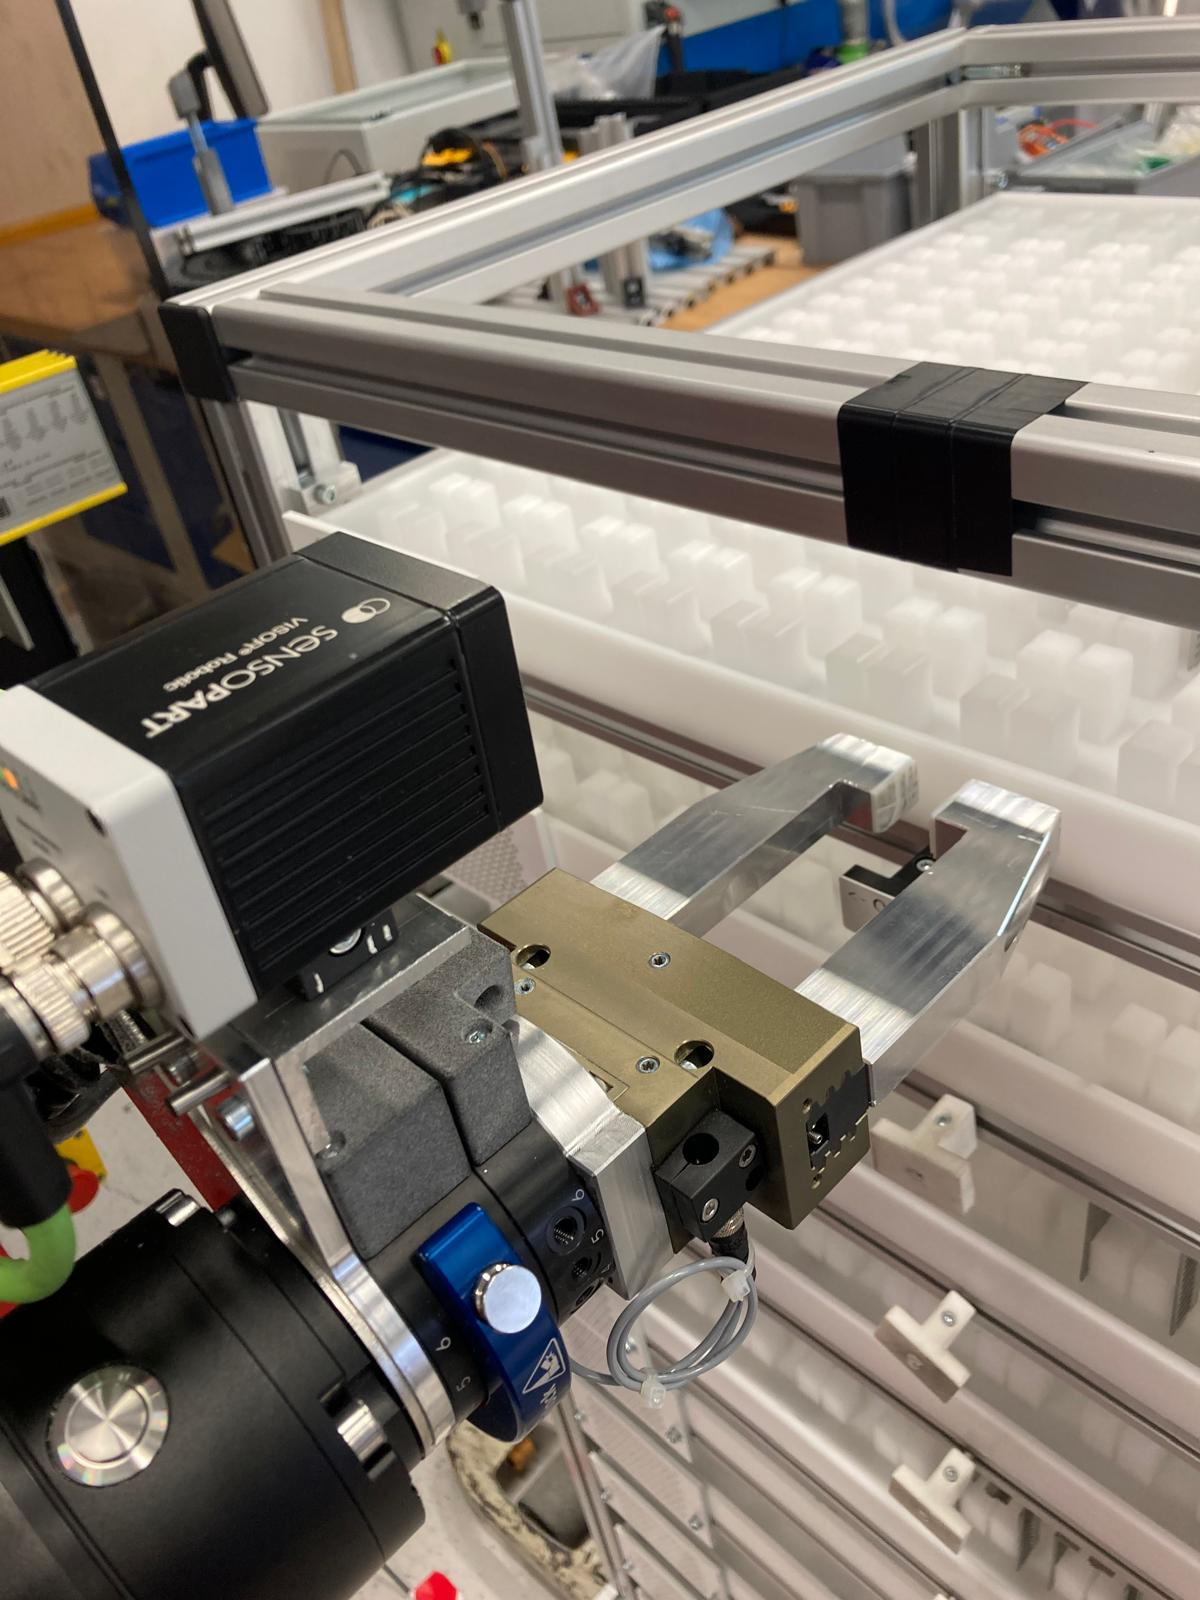
\includegraphics[width=\textwidth]{figures/shelf-control/reach-handle.jpeg}
        \caption{Reach shelf handle}
        \label{subfig:reach-handle}
    \end{subfigure}\hspace{0.1cm}
    \begin{subfigure}[b]{0.32\textwidth}
        \centering
        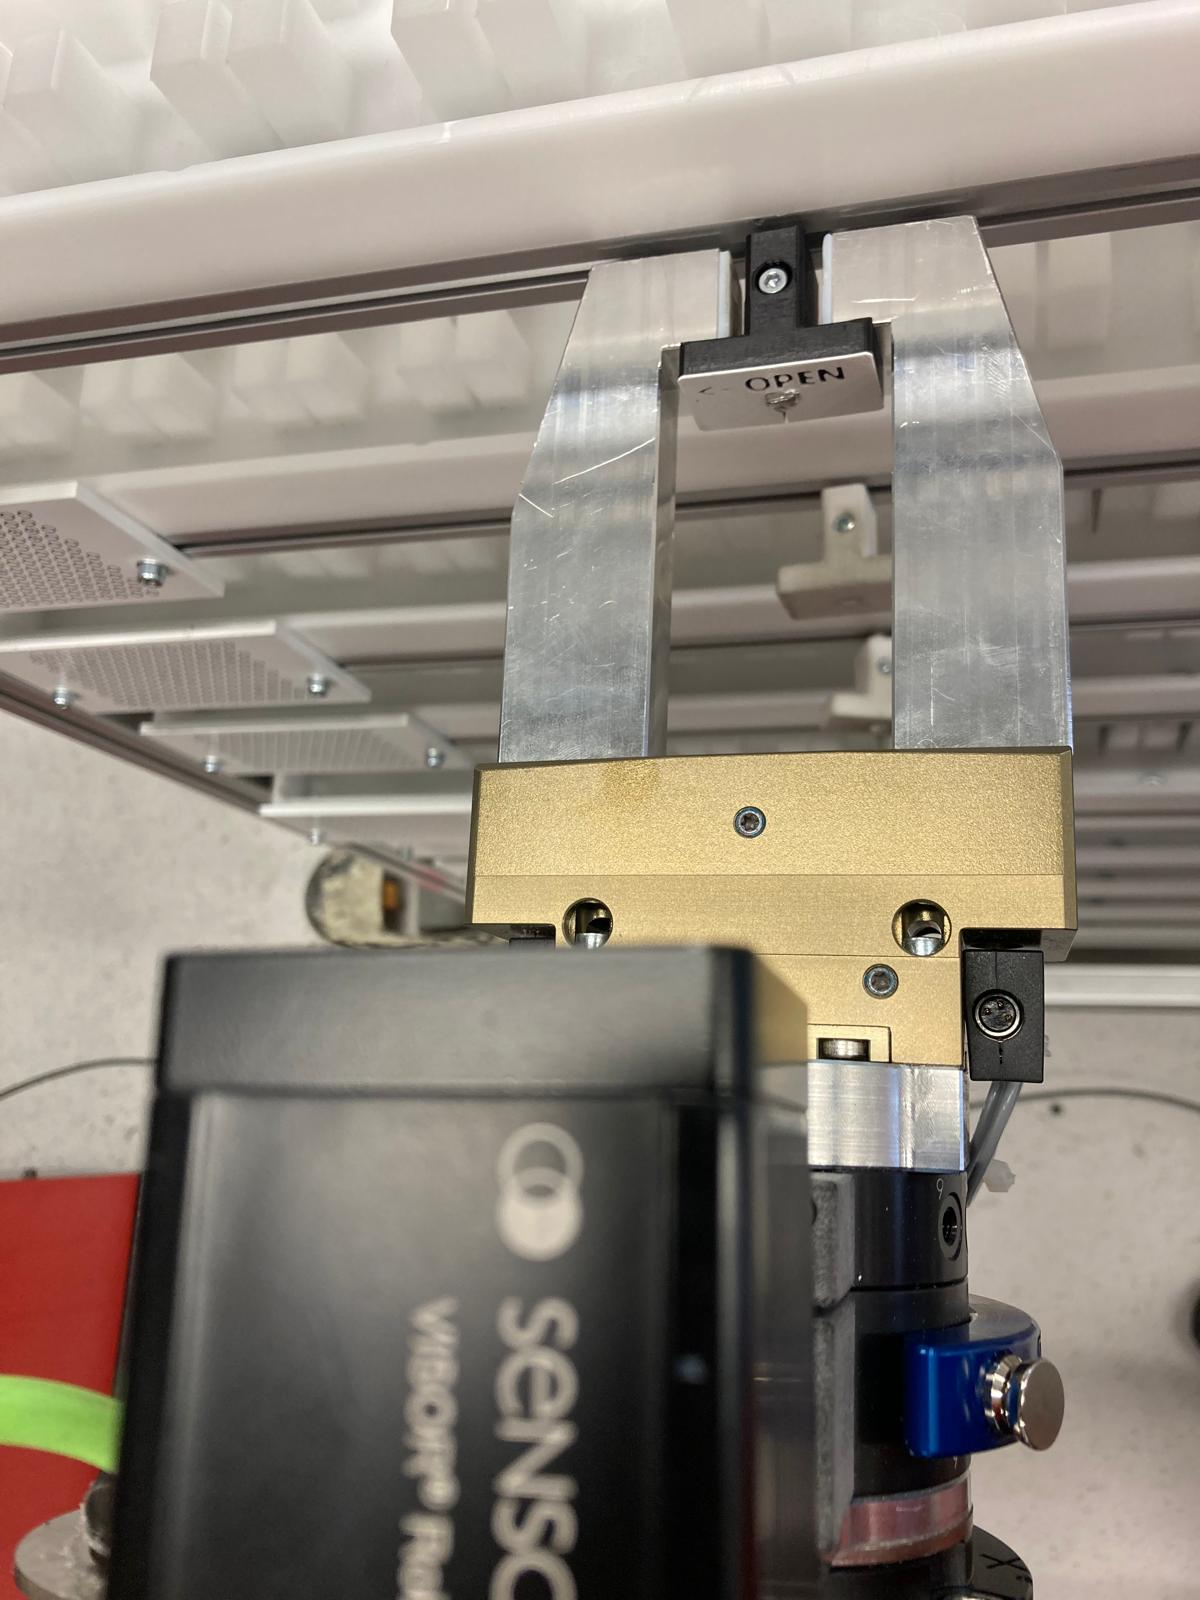
\includegraphics[width=\textwidth]{figures/shelf-control/hold-handle.jpeg}
        \caption{grasp handle with gripper}
        \label{subfig:grasp-handle}
    \end{subfigure}\hspace{0.1cm}
    \vspace{1cm}
    \begin{subfigure}[b]{0.32\textwidth}
        \centering
        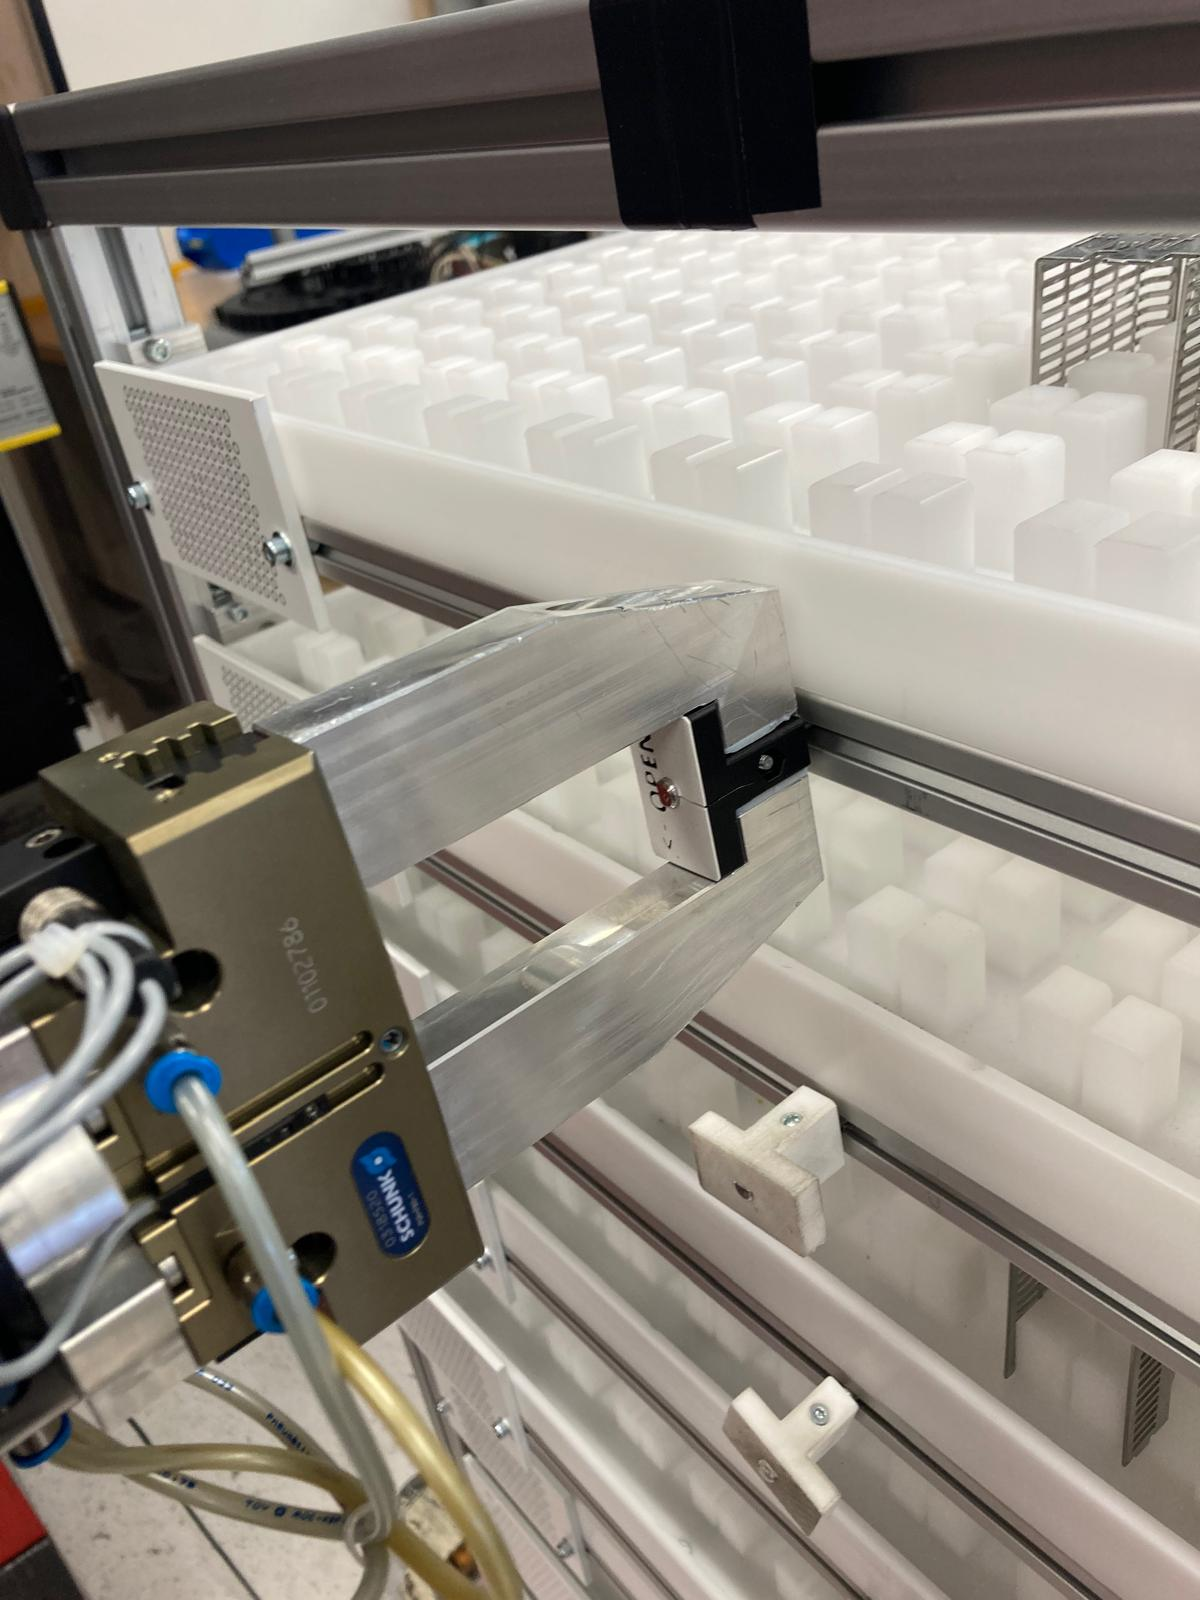
\includegraphics[width=\textwidth]{figures/shelf-control/open-handle.jpeg}
        \caption{Turn handle 100\textdegree{} to open drawer}
        \vspace{-0.45cm}
        \label{subfig:turn-open}
    \end{subfigure}\hspace{0.1cm}
    \begin{subfigure}[b]{0.32\textwidth}
        \centering
        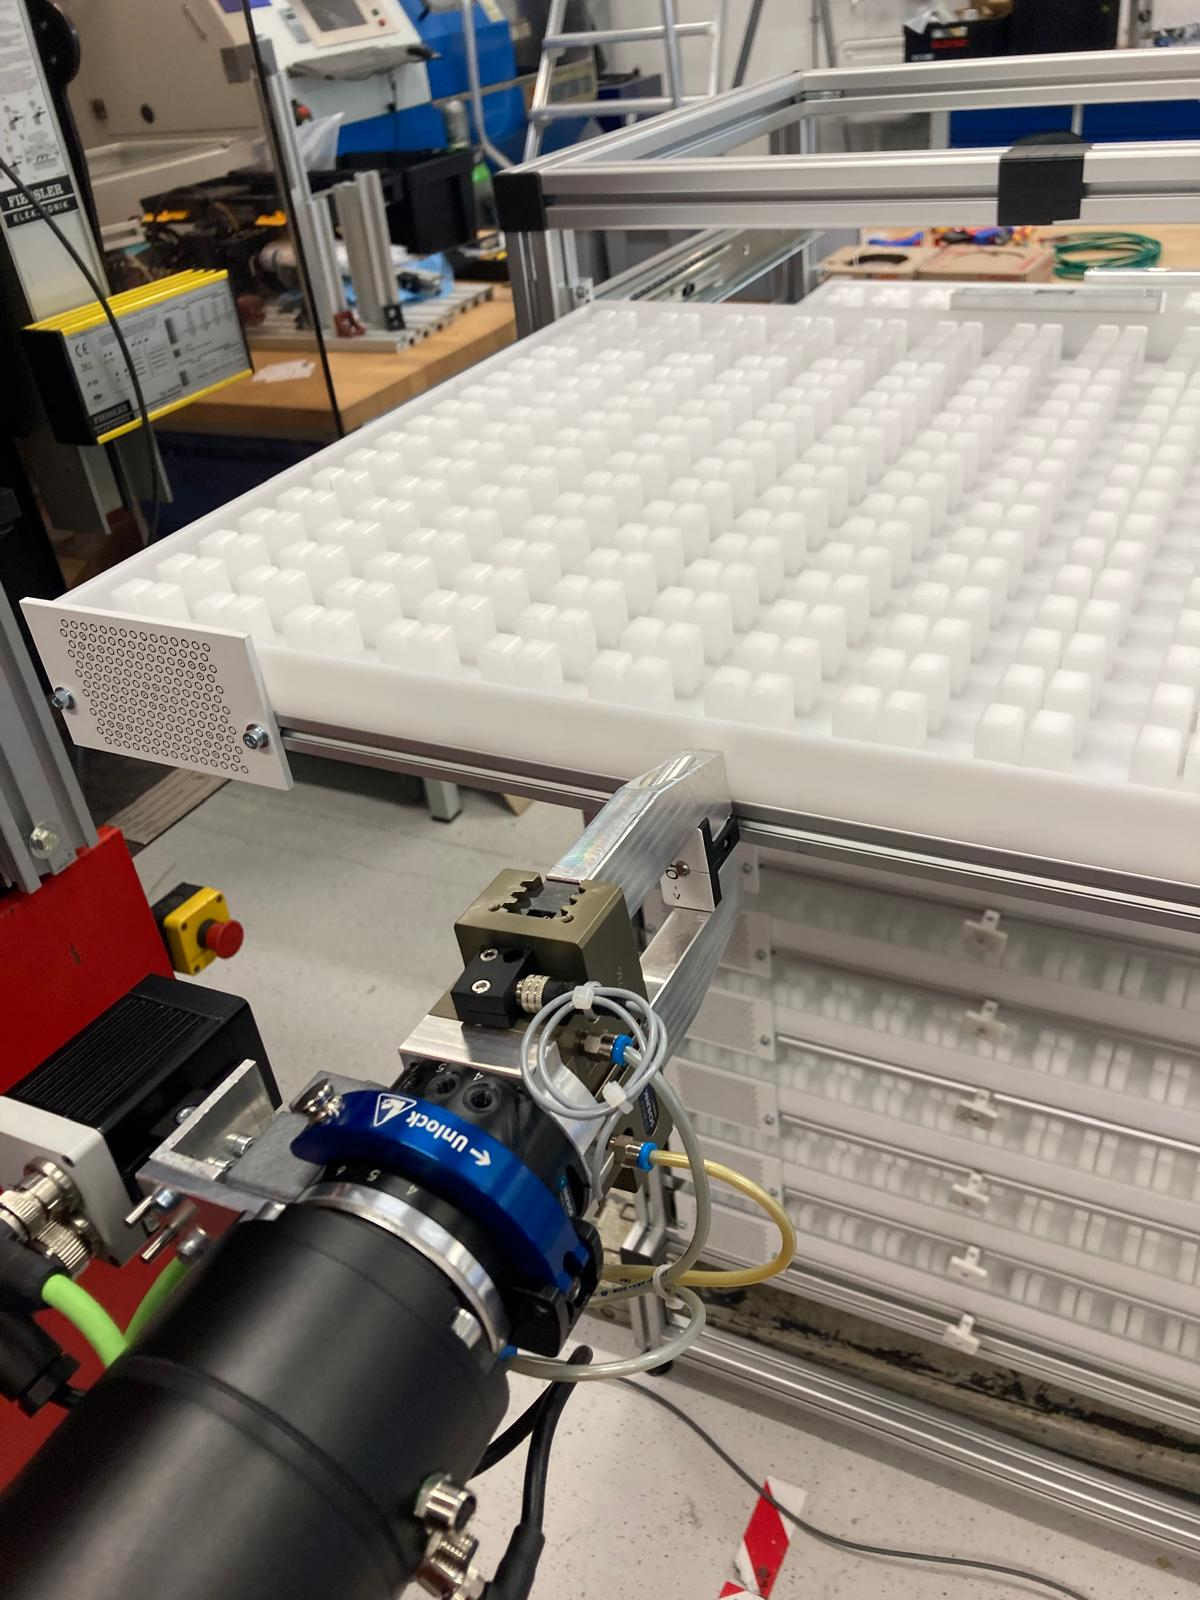
\includegraphics[width=\textwidth]{figures/shelf-control/open-drawer.jpeg}
        \caption{open drawer}
        \vspace{0.45cm}
        \label{fig:open-drawer}
    \end{subfigure}\hspace{0.1cm}
    \vspace{0.75cm}
    \begin{subfigure}[b]{0.32\textwidth}
        \centering
        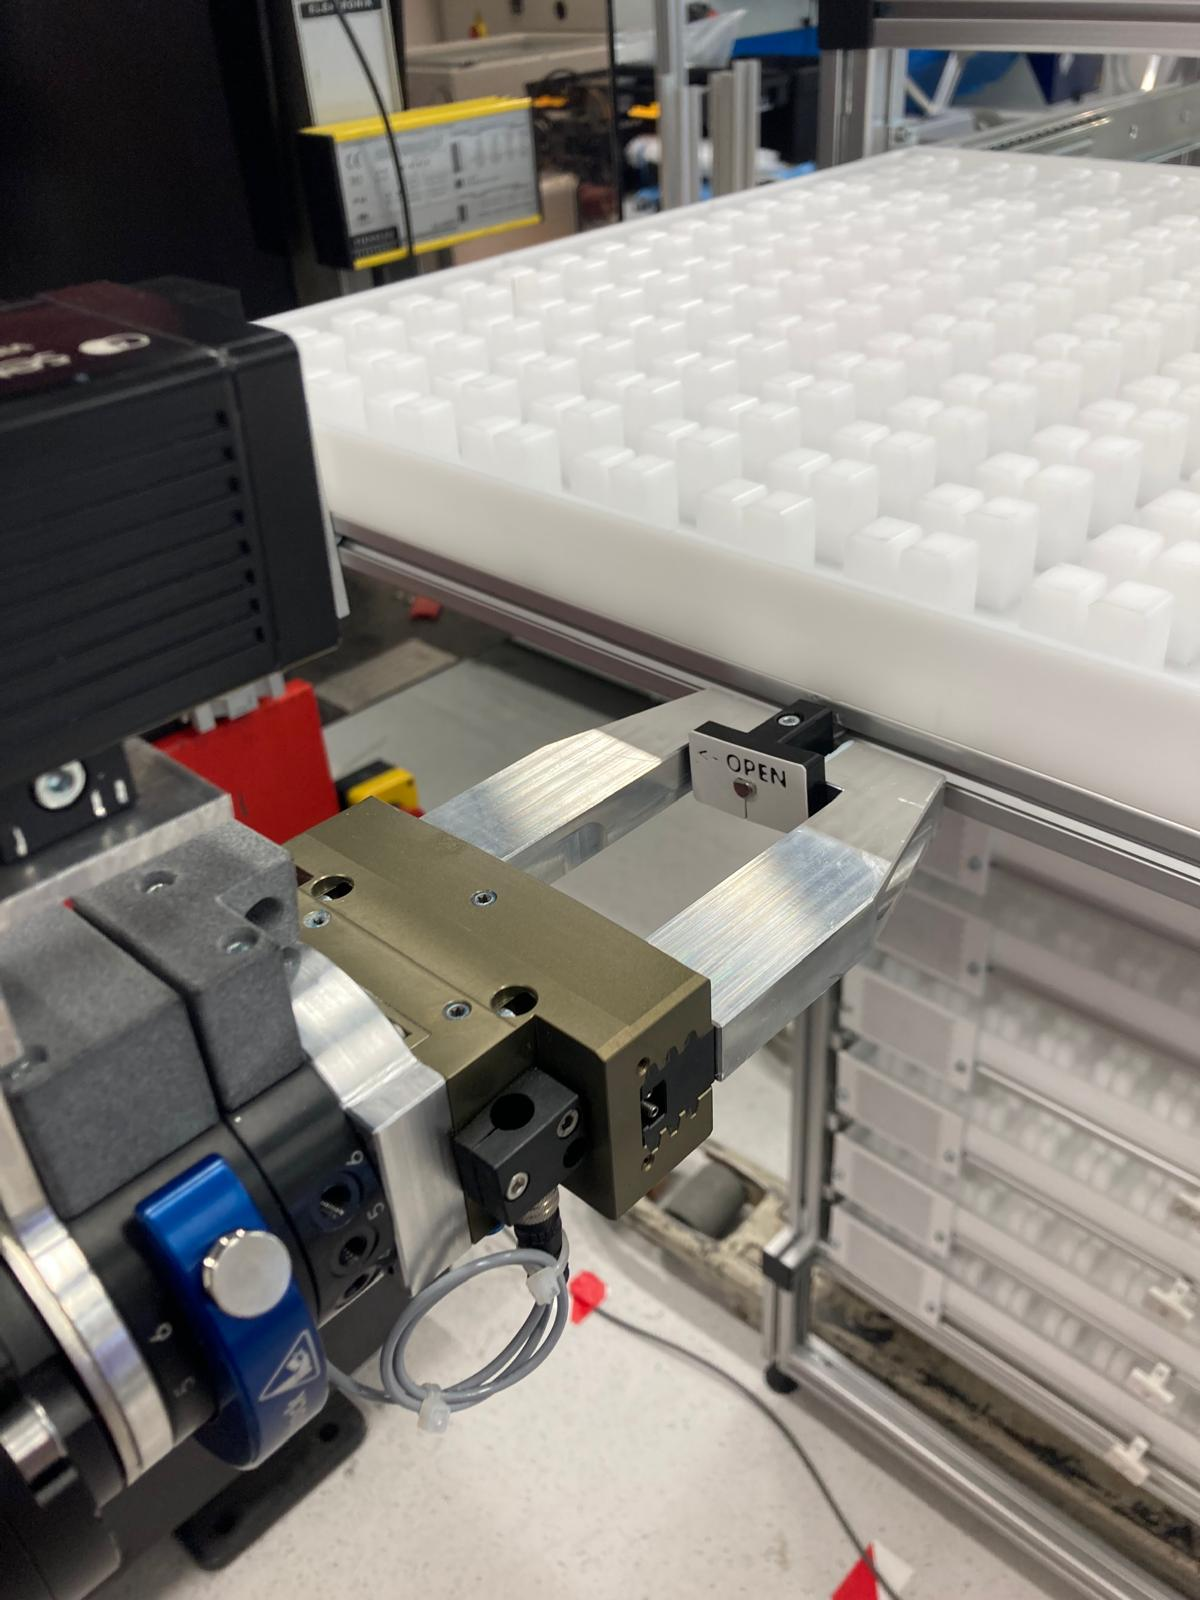
\includegraphics[width=\textwidth]{figures/shelf-control/close-handle.jpeg}
        \caption{Turn handle -100\textdegree{} to fix drawer in open position}
        \label{fig:close-handle}
    \end{subfigure}\hspace{0.1cm}
    \begin{subfigure}[b]{0.32\textwidth}
        \centering
        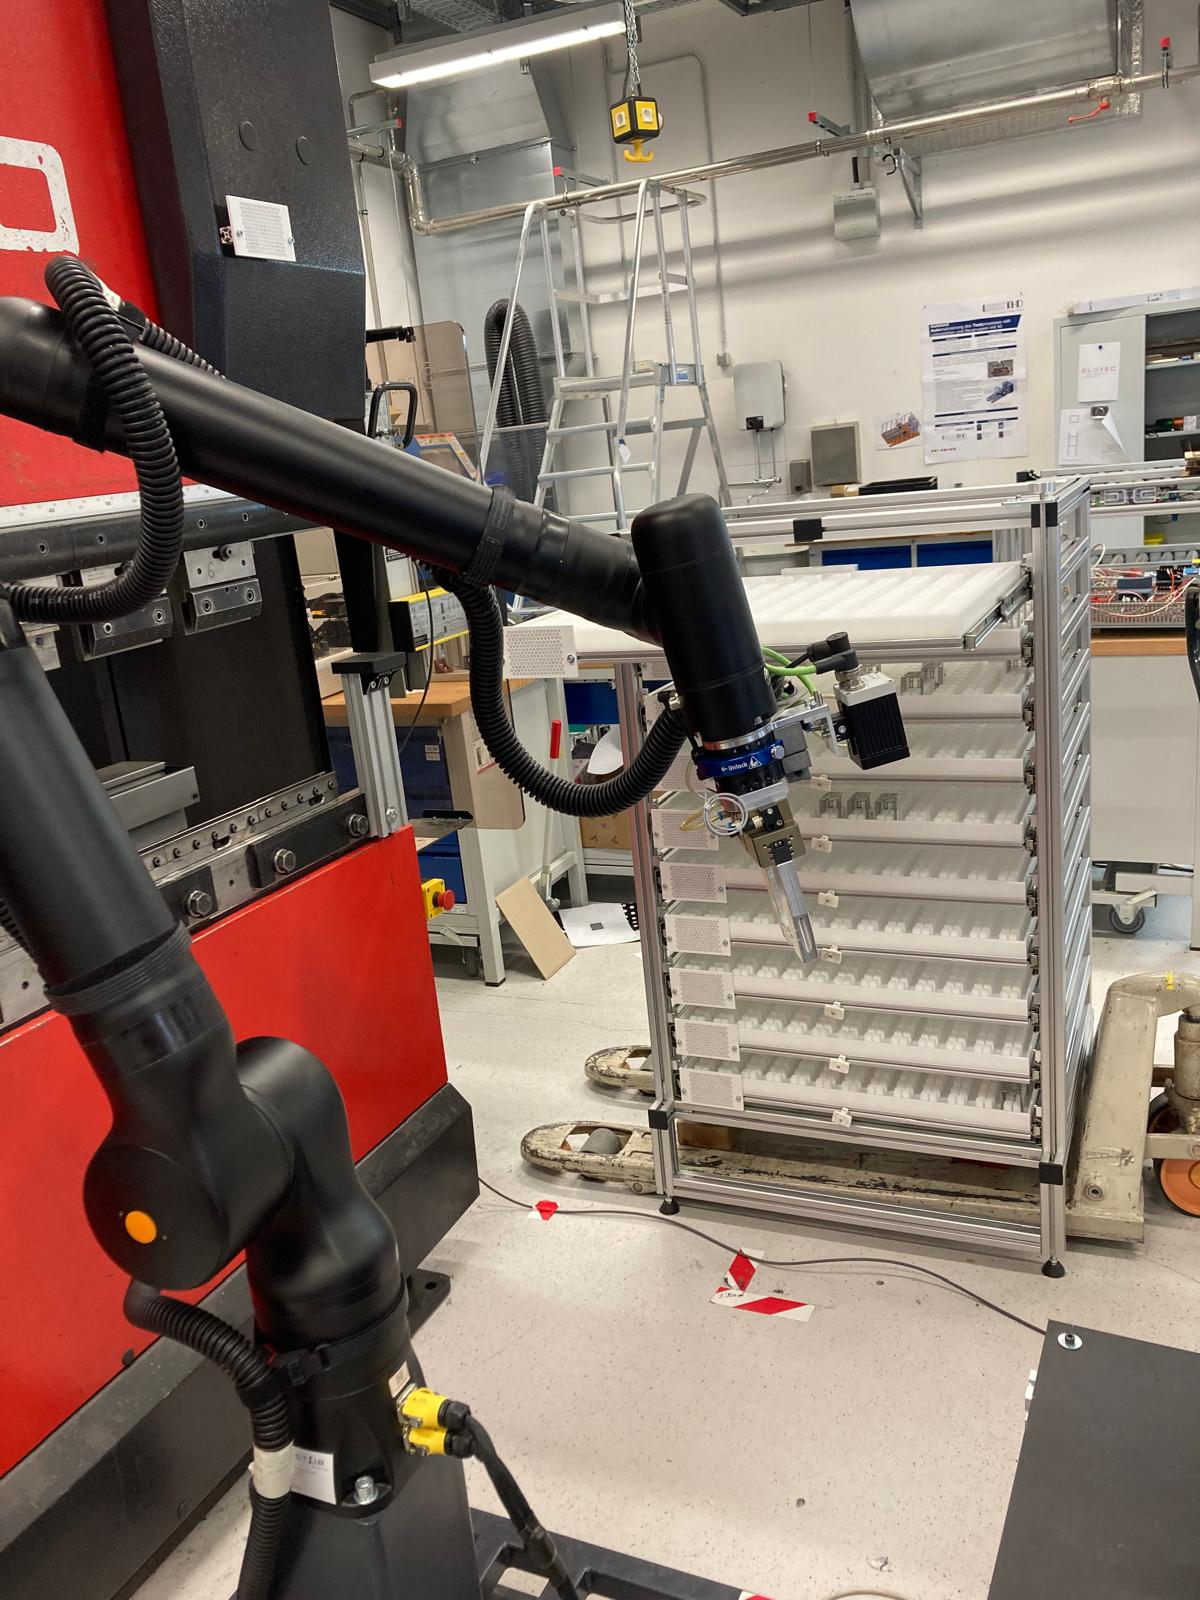
\includegraphics[width=\textwidth]{figures/shelf-control/drawer-opened.jpeg}
        \caption{Robot ready with drawer open}
        \label{subfig:drawer-opened}
    \end{subfigure}\hspace{0.1cm}
    \caption{Opening a shelf drawer for placement of bent sheet metal parts}
    \label{fig:shelf-control}
\end{figure}







\section{Calibration}

Calibration is a crucial procedure in the development of 
an automated robotic workcell, ensuring that all components
operate accurately and in harmony.


\begin{figure}[h]
    \centering
    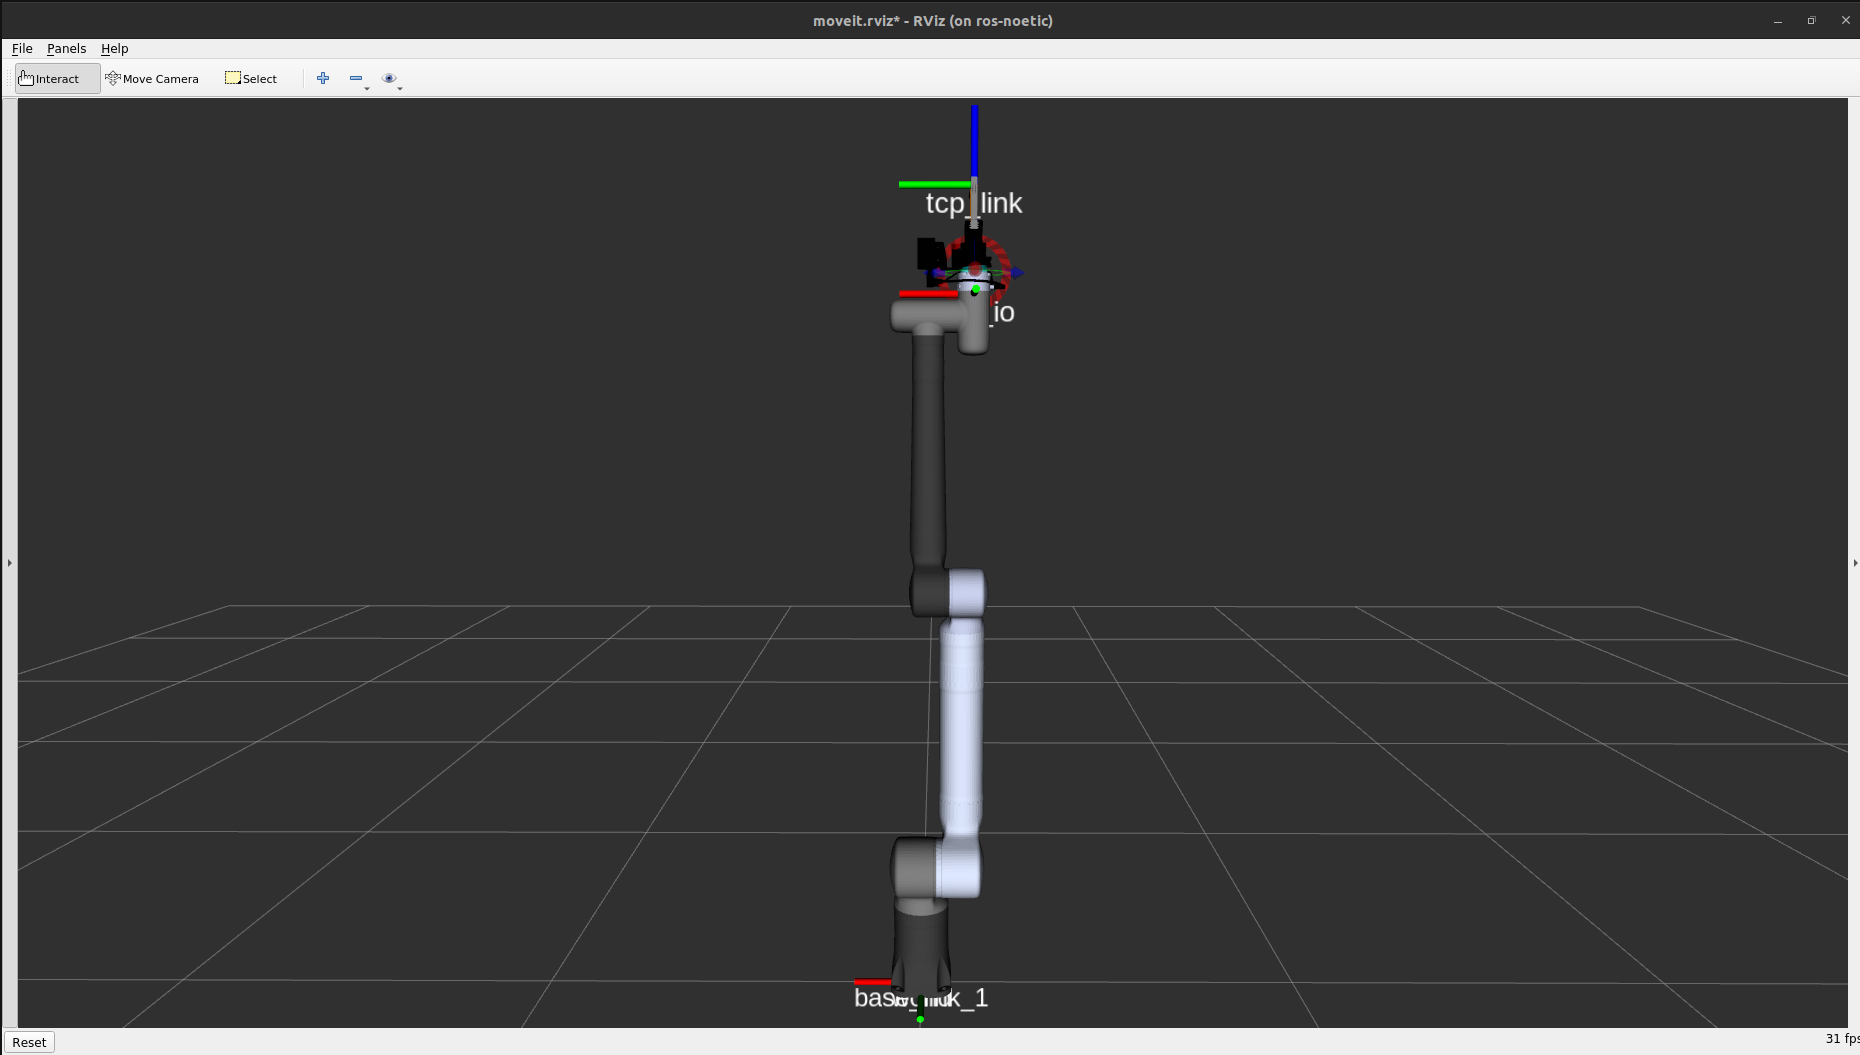
\includegraphics[width=\textwidth]{6. System Integration and Testing/6.2 Calibration Procedures/tcp.PNG}
    \caption{TCP is set at the end of gripper at a distance of 216mm from robot TOOL-IO}
    \label{fig:tcp}
\end{figure}




\subsection{Robot Calibration}
Robot calibration ensures that the Kassow robot can accurately position its end effector for loading, bending, and unloading metal sheets. This involves:

\begin{itemize}
    \item \textbf{Kinematic Calibration}: Adjusting the robot's kinematic model to correct any discrepancies between the theoretical model and the actual hardware. This includes measuring and compensating for joint offsets, link lengths, and joint angles.
    \item \textbf{Tool Center Point (TCP) Calibration}: Determining the exact position of the end effector or tool relative to the robot’s last joint. This is crucial for precise manipulation of metal sheets.
    \item \textbf{Workspace Calibration}: Defining the robot's operational workspace and ensuring that all tasks are performed within this defined area, avoiding collisions and ensuring smooth operation.
\end{itemize}

The KR1410 is already calibrated from the factory and does not need to be setup. Though in simulation, robot kinematic model is generated from the URDF and needs to be updated to match the real hardware.

\subsection{Camera Calibration}
The "Hand-Eye calibration (Robotics)" calibration method is used to determine the
reference between "Hand" (TCP) and "Eye" Camera coordinate system
(position and orientation) when the VISOR\textsuperscript{\textregistered} is attached to the gripper.
This allows different image acquisition positions and still to output the object positions
in robot coordinates directly from the camera.
\cite[page 102]{visor_user_manual}

\begin{figure}[h]
    \centering
    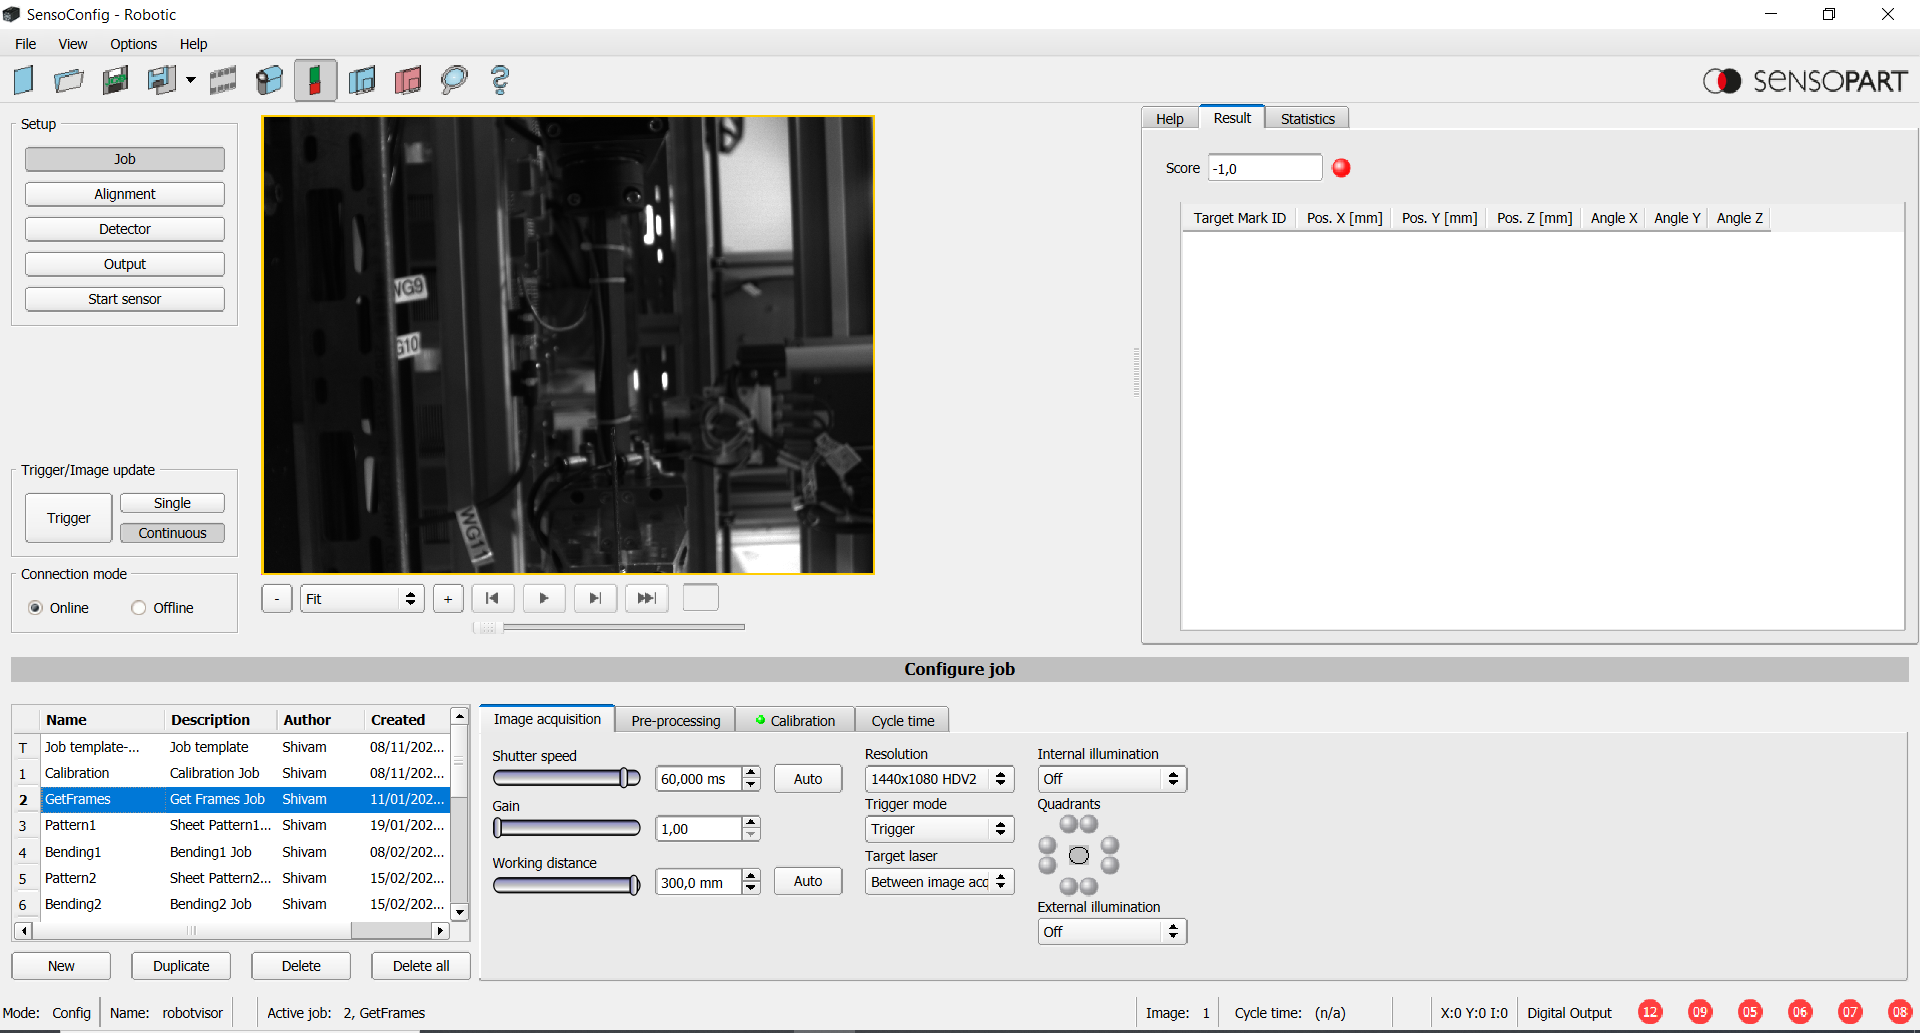
\includegraphics[width=0.9\textwidth]{6. System Integration and Testing/6.2 Calibration Procedures/shutter_speed.PNG}
    \caption{A working distance of 300mm is set for the robotic camera}
    \label{fig:working-distance}
\end{figure}

Camera calibration is essential for the accurate detection of metal sheets and measurement of bending angles. The process involves:

\begin{itemize}
    \item \textbf{Intrinsic Calibration}: Determining the camera's internal parameters, such as focal length, optical center, and lens distortion. This is typically achieved using a calibration target (e.g., a checkerboard pattern) and specialized software tools.
    \item \textbf{Extrinsic Calibration}: Establishing the camera's position and orientation relative to the robot or the workcell. This involves aligning the camera's coordinate system with the robot’s coordinate system to ensure accurate detection and measurement.
\end{itemize}

\subsection{Sensor Calibration}
Laser sensor is added to the bending machine to measure the distance between the tool and die with the reproducibility in the range of 10\textmu m. This sensor help in coordinating the bending timings between the bending machine and the robot. This sensor also requires a baseline or zero point to eliminate any offsets or biases in their readings.

\subsection{Calibration Procedures}

The calibration process is automated within the robot program
such that operator could request to re-calibrate the camera w.r.t
robot TCP from the touch panel. This allows to update the image quality as it degrades over time. 
The robot finishes the current
bending operation and then in next cycle, start with the auto-calibration.

\begin{figure}[h]
    \centering
    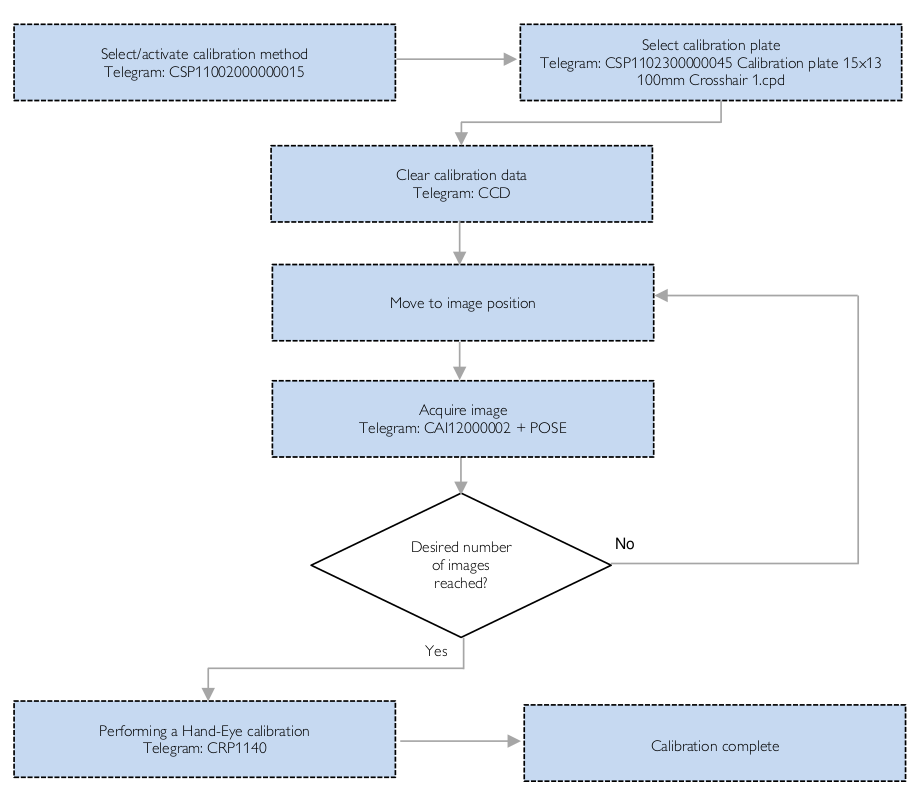
\includegraphics[width=\textwidth]{6. System Integration and Testing/6.2 Calibration Procedures/graph.png}
    \caption{Calibration procedure using telegram}
    \label{calib-graph:tcp}
\end{figure}

The calibration process involves several systematic steps:

\begin{enumerate}
    \item \textbf{Setup Calibration Targets}: Place calibration targets within the robot’s workspace and at specific positions that the cameras will observe.
    \item \textbf{Data Collection}: Use the robot and cameras to collect data from the calibration targets. This includes moving the robot through its range of motion and capturing images from different angles.
    \item \textbf{Parameter Estimation}: Use calibration software to estimate the parameters of the robot’s kinematic model, the intrinsic and extrinsic parameters of the cameras, and the characteristics of any other sensors.
    \item \textbf{Validation}: Verify the calibration by performing tasks that require high precision and checking the accuracy of the results. Adjust calibration parameters as needed based on validation results.
    \item \textbf{Documentation}: Record the calibration parameters and procedures for future reference and troubleshooting.
\end{enumerate}





\section{Performance Evaluation}
After the integration tests of each bending operation, the program for each bending stage is compiled together to create a main program which cycles through all bending operations for the test sheet metal part. After all six bending operations on the test part, KR1410 robot loads the sheet in the drawer of storage station.
The main program is based on the flowchart \ref{tab:flowchart} and uses the variables shared with the PLC (as shown in table \ref{tab:kr1410-to-plc} and \ref{tab:plc-to-kr1410}) to perform the bending.

A cycle starts when a new sheet is requested by the KR1410. It ends with the placement of bent sheet in the drawer of the shelf. After all the optimizations for trajectory planning in teach pendant, the cycle time comes out to be around 4 minutes and 10 seconds with inspection active. Without any inspection, the cycle time reduces to 3 minutes and 40 seconds.

The performance of the bending process is evaluated in the following sections using the calibration results, inspection assessment and reviewing the bending operation.

\section{Calibration Results}
\label{sec:calibration-results}
Calibration is fundamental to ensuring the accuracy and reliability of an automated robotic workcell. The calibration process takes exactly 98 seconds for the robot. Proper calibration ensures that the robot operate with high accuracy, thus reducing variability in the bent sheet metal part.

Figure \ref{fig:calibration-parameters} shows the calibration parameters after an automatic calibration. The field of view is 100\% with a resolution of 0.1564 mm/pixel.

\begin{figure}[h]
    \centering
    \begin{subfigure}{0.48\textwidth}
        \centering
        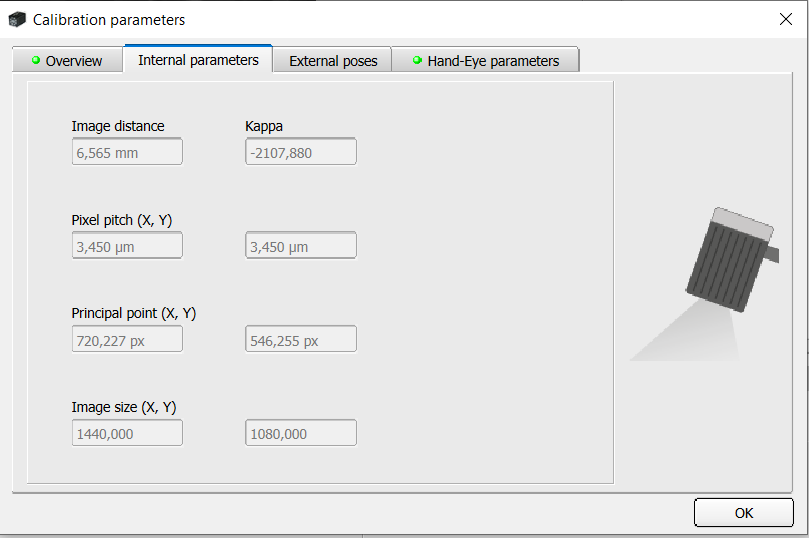
\includegraphics[width=\textwidth]{figures/001calibration/internal_parameters.PNG}
        \caption{Internal parameters}
        \label{subfig:internal-parameters}
    \end{subfigure}\hspace{0cm}
    \begin{subfigure}{0.48\textwidth}
        \centering
        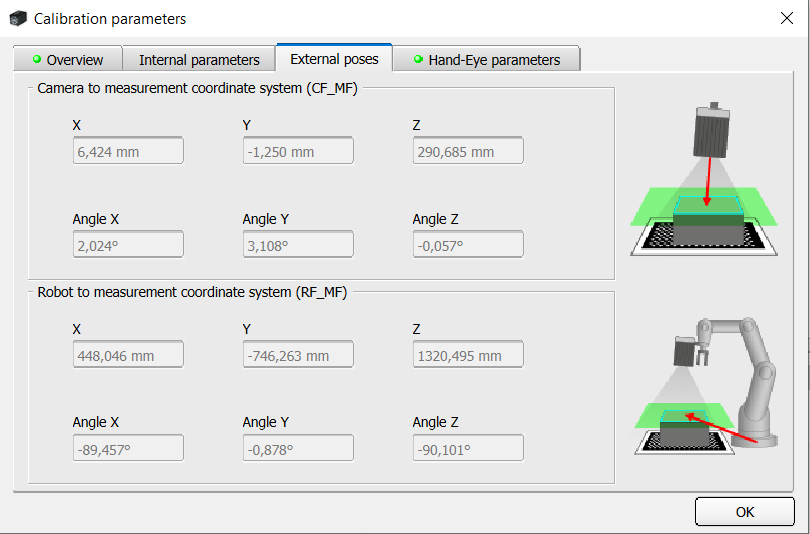
\includegraphics[width=\textwidth]{figures/001calibration/external_poses.PNG}
        \caption{External poses}
        \label{subfig:external-poses}
    \end{subfigure}
    \begin{subfigure}{0.48\textwidth}
        \centering
        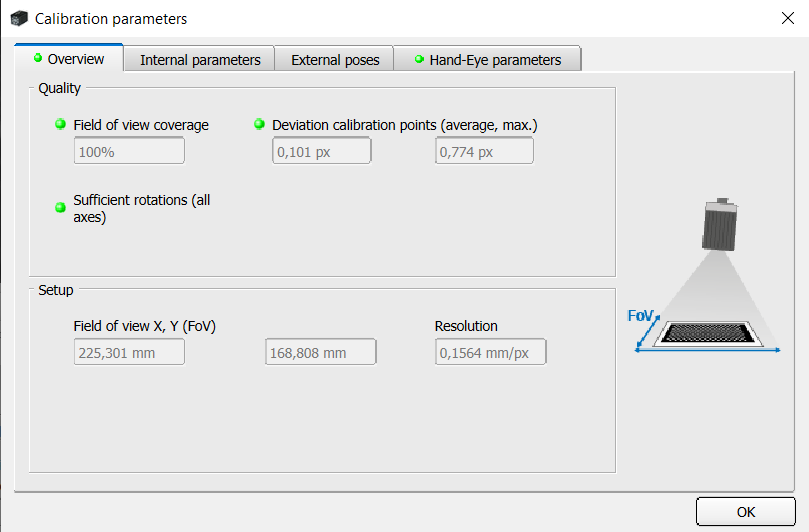
\includegraphics[width=\textwidth]{figures/001calibration/fov.PNG}
        \caption{Field of view}
        \label{subfig:fov}
    \end{subfigure}
    \begin{subfigure}{0.48\textwidth}
        \centering
        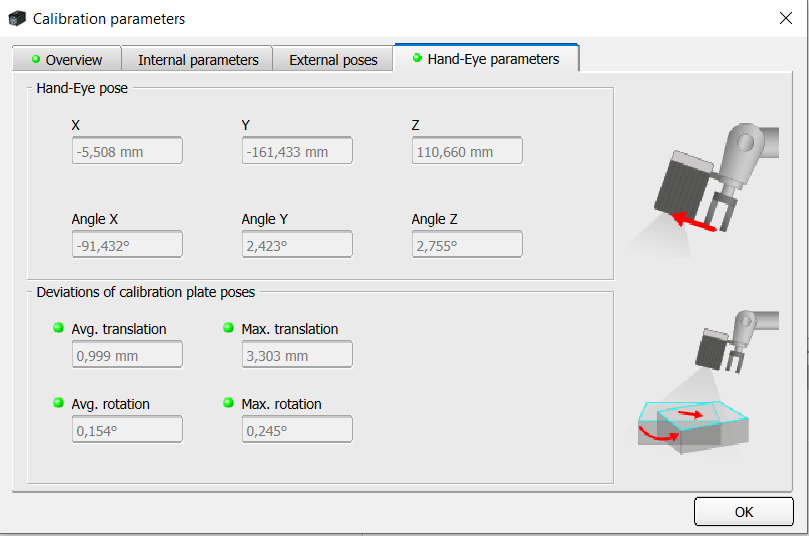
\includegraphics[width=\textwidth]{figures/001calibration/hand-eye_parameters.PNG}
        \caption{Hand-eye parameters}
        \label{subfig:hand-eye-parameters}
    \end{subfigure}
    \caption{Calibration parameters}
    \label{fig:calibration-parameters}
\end{figure}


By establishing rigorous calibration procedures, the automated robotic workcell can achieve optimal performance, ensuring that the bending process is executed with high precision and reliability.  The \hyperref[acro:KR]{KR1410} robot only has a repeatability of 0.1 mm. After the \hyperref[acro:TCP]{TCP} calibration, the bending process has a repeatability of 0.5 mm, which is still better than a human operator.

\FloatBarrier  % Force all figures of the first section to be placed before the next section

\section{Inspection Assessment}
\label{sec:inspection-assessment}
The inspection of only four bending operations out of six bendings are required for the test part. Figure \ref{fig:bending-inspection} shows these inspection camera images upon trigger. Figure \ref{subfig:inspection-1}, \ref{subfig:inspection-5} and \ref{subfig:inspection-6} tests the bending operation of 90\textdegree which is performed at bending station 1. Figure \ref{subfig:inspection-2} is the testing of bending of 135\textdegree which happens at bending station 2.

Table \ref{tab:bending-data} shows the bending angles as measured by the inspection camera for ten sheet metal parts. The angle measurement is pretty close to each other. The angle is measured by the light reflected by the edge of sheet metal part. Because of different surface roughness and impurities on surface, there is slight deviation in the bending angles measured. A tolerance of 90$\pm5$\textdegree{} is set for the bending 1, bending 5 and bending 6. For bending 2, a tolerance of 135$\pm10$\textdegree{} is set. These tolerance values can be adjusted on the SIMATIC HMI.

\begin{figure}[h]
    \centering
    \begin{subfigure}{0.48\textwidth}
        \centering
        \includegraphics[width=\textwidth]{figures/008_inspection/inpection_1_overlay2.png}
        \caption{bending  operation 1}
        \label{subfig:inspection-1}
        \vspace{0.5cm}
    \end{subfigure}\hspace{0.25cm}
    \begin{subfigure}{0.48\textwidth}
        \centering
        \includegraphics[width=\textwidth]{figures/008_inspection/inspection_2_overlay.png}
        \caption{bending operation 2}
        \label{subfig:inspection-2}
        \vspace{0.5cm}
    \end{subfigure}\hspace{0.25cm}
    \begin{subfigure}{0.48\textwidth}
        \centering
        \includegraphics[width=\textwidth]{figures/008_inspection/inspection_5_overlay_cleanup.png}
        \caption{bending operation 5}
        \label{subfig:inspection-5}
        \vspace{0.25cm}
    \end{subfigure}\hspace{0.25cm}
    \begin{subfigure}{0.48\textwidth}
        \centering
        \includegraphics[width=\textwidth]{figures/008_inspection/inspection_6_overlay_cleanup.png}
        \caption{bending operation 6}
        \label{subfig:inspection-6}
        \vspace{0.25cm}
    \end{subfigure}\hspace{0.25cm}
    \caption{Inspection after (a) bending 1 (b) bending 2 (c) bending 5 (d) bending 6}
    \label{fig:bending-inspection}
\end{figure}

\begin{table}[ht]
    \centering
    \small
    \renewcommand{\arraystretch}{1.2} % Adjusts row height
    \begin{tabular}{llcccc}
        & \textbf{Bending 1} & \textbf{Bending 2} & \textbf{Bending 5} & \textbf{Bending 6} \\
        \hline
        & 89.16801 & 133.412 & 88.84901 & 87.79301 \\
        & 89.29201 & 133.048 & 88.77    & 87.36501 \\
        & 89.381   & 133.548 & 88.785   & 87.257   \\
        & 89.344   & 132.454 & 88.928   & 87.561   \\
        & 89.43401 & 133.184 & 89.217   & 87.302   \\
        & 88.402   & 132.967 & 89.176   & 88.19701 \\
        & 89.10001 & 134.015 & 88.926   & 88.276   \\
        & 90.08801 & 132.146 & 89.023   & 87.58801 \\
        & 90.08701 & 134.084 & 87.966   & 87.75301 \\
        & 89.995   & 135.314 & 88.34801 & 87.526   \\
        \hline
    \end{tabular}
    \caption{Bending angle as measured by inspection camera}
    \label{tab:bending-data}
\end{table}

The bending angles measured by the inspection camera are saved by the PLC in a \textit{.csv} file. Simatic HMI also shows the current cycle bending angles for the operator to overview the current status of bending operation. This \textit{.csv} file provides insights in the quality of bending process over time. It is evident from the angles captured that the bending process is consistent over time, without any requirement for a new calibration.
\FloatBarrier  % Force all figures of the first section to be placed before the next section

\section{Bending Operation Review}
\label{sec:calibration-results}
Figure \ref{fig:final-bent-part} shows the final bent sheet metal part that is sent to the project partner for assessment and measurement. The test part is scanned in a 3D scanner for measurement of all bending angles and surface structure. There are no discrepancies found in any of the test parts bent by the KR1410 robotic workcell. This shows that the inspection camera is working correctly and the angle difference between two parts is only due to surface imperfections. Hence, a bigger tolerance in the inspection camera angle measurement still gives correctly bent part.

\begin{figure}[h]
    \centering
    \begin{subfigure}{0.48\textwidth}
        \centering
        \includegraphics[width=\textwidth]{figures/bending/final-part02.png}
        \caption{}
        \label{subfig:final-part1}
        \vspace{0.5cm}
    \end{subfigure}\hspace{0.25cm}
    \begin{subfigure}{0.48\textwidth}
        \centering
        \includegraphics[width=\textwidth]{figures/bending/final-part01.png}
        \caption{}
        \label{subfig:final-part2}
        \vspace{0.5cm}
    \end{subfigure}\hspace{0.25cm}

    \caption{Final bent sheet metal part (a) top view (b) bottom view}
    \label{fig:final-bent-part}
\end{figure}
\FloatBarrier  % Force all figures of the first section to be placed before the next section







\chapter{Experimental Results}
\label{chap:results}

\setcounter{section}{0}
\setcounter{subsection}{0}

% \section{Performance Evaluation}
\label{sec:performance}
After the integration tests of each bending operation, the program for each bending stage is compiled together to create a main program which cycles through all bending operations for the test sheet metal part. After all six bending operations on the test part, KR1410 robot loads the sheet in the drawer of storage station.
The main program is based on the flowchart \ref{tab:flowchart} and uses the variables shared with the PLC (as shown in table \ref{tab:kr1410-to-plc} and \ref{tab:plc-to-kr1410}) to perform the bending.

A cycle starts when a new sheet is requested by the KR1410. It ends with the placement of bent sheet in the drawer of the shelf. After all the optimizations for trajectory planning in teach pendant, the cycle time comes out to be around 4 minutes and 10 seconds with inspection active. Without any inspection, the cycle time reduces to 3 minutes and 40 seconds.

The performance of the bending process is evaluated in the following sections using the calibration results, inspection assessment and reviewing the bending operation.

\section{Calibration Results}
\label{sec:calibration-results}
Calibration is fundamental to ensuring the accuracy and reliability of an automated robotic workcell. The calibration process takes exactly 98 seconds for the robot. Proper calibration ensures that the robot operate with high accuracy, thus reducing variability in the bent sheet metal part.

Figure \ref{fig:calibration-parameters} shows the calibration parameters after an automatic calibration. The field of view is 100\% with a resolution of 0.1564 mm/pixel.

\begin{figure}[h]
    \centering
    \begin{subfigure}{0.48\textwidth}
        \centering
        \includegraphics[width=\textwidth]{figures/001calibration/internal_parameters.PNG}
        \caption{Internal parameters}
        \label{subfig:internal-parameters}
    \end{subfigure}\hspace{0cm}
    \begin{subfigure}{0.48\textwidth}
        \centering
        \includegraphics[width=\textwidth]{figures/001calibration/external_poses.PNG}
        \caption{External poses}
        \label{subfig:external-poses}
    \end{subfigure}
    \begin{subfigure}{0.48\textwidth}
        \centering
        \includegraphics[width=\textwidth]{figures/001calibration/fov.PNG}
        \caption{Field of view}
        \label{subfig:fov}
    \end{subfigure}
    \begin{subfigure}{0.48\textwidth}
        \centering
        \includegraphics[width=\textwidth]{figures/001calibration/hand-eye_parameters.PNG}
        \caption{Hand-eye parameters}
        \label{subfig:hand-eye-parameters}
    \end{subfigure}
    \caption{Calibration parameters}
    \label{fig:calibration-parameters}
\end{figure}


By establishing rigorous calibration procedures, the automated robotic workcell can achieve optimal performance, ensuring that the bending process is executed with high precision and reliability.  The \hyperref[acro:KR]{KR1410} robot only has a repeatability of 0.1 mm. After the \hyperref[acro:TCP]{TCP} calibration, the bending process has a repeatability of 0.5 mm, which is still better than a human operator.

\FloatBarrier  % Force all figures of the first section to be placed before the next section

\section{Inspection Assessment}
\label{sec:inspection-assessment}
The inspection of only four bending operations out of six bendings are required for the test part. Figure \ref{fig:bending-inspection} shows these inspection camera images upon trigger. Figure \ref{subfig:inspection-1}, \ref{subfig:inspection-5} and \ref{subfig:inspection-6} tests the bending operation of 90\textdegree which is performed at bending station 1. Figure \ref{subfig:inspection-2} is the testing of bending of 135\textdegree which happens at bending station 2.

Table \ref{tab:bending-data} shows the bending angles as measured by the inspection camera for ten sheet metal parts. The angle measurement is pretty close to each other. The angle is measured by the light reflected by the edge of sheet metal part. Because of different surface roughness and impurities on surface, there is slight deviation in the bending angles measured. A tolerance of 90$\pm5$\textdegree{} is set for the bending 1, bending 5 and bending 6. For bending 2, a tolerance of 135$\pm10$\textdegree{} is set. These tolerance values can be adjusted on the SIMATIC HMI.

\begin{figure}[h]
    \centering
    \begin{subfigure}{0.48\textwidth}
        \centering
        \includegraphics[width=\textwidth]{figures/008_inspection/inpection_1_overlay2.png}
        \caption{bending  operation 1}
        \label{subfig:inspection-1}
        \vspace{0.5cm}
    \end{subfigure}\hspace{0.25cm}
    \begin{subfigure}{0.48\textwidth}
        \centering
        \includegraphics[width=\textwidth]{figures/008_inspection/inspection_2_overlay.png}
        \caption{bending operation 2}
        \label{subfig:inspection-2}
        \vspace{0.5cm}
    \end{subfigure}\hspace{0.25cm}
    \begin{subfigure}{0.48\textwidth}
        \centering
        \includegraphics[width=\textwidth]{figures/008_inspection/inspection_5_overlay_cleanup.png}
        \caption{bending operation 5}
        \label{subfig:inspection-5}
        \vspace{0.25cm}
    \end{subfigure}\hspace{0.25cm}
    \begin{subfigure}{0.48\textwidth}
        \centering
        \includegraphics[width=\textwidth]{figures/008_inspection/inspection_6_overlay_cleanup.png}
        \caption{bending operation 6}
        \label{subfig:inspection-6}
        \vspace{0.25cm}
    \end{subfigure}\hspace{0.25cm}
    \caption{Inspection after (a) bending 1 (b) bending 2 (c) bending 5 (d) bending 6}
    \label{fig:bending-inspection}
\end{figure}

\begin{table}[ht]
    \centering
    \small
    \renewcommand{\arraystretch}{1.2} % Adjusts row height
    \begin{tabular}{llcccc}
        & \textbf{Bending 1} & \textbf{Bending 2} & \textbf{Bending 5} & \textbf{Bending 6} \\
        \hline
        & 89.16801 & 133.412 & 88.84901 & 87.79301 \\
        & 89.29201 & 133.048 & 88.77    & 87.36501 \\
        & 89.381   & 133.548 & 88.785   & 87.257   \\
        & 89.344   & 132.454 & 88.928   & 87.561   \\
        & 89.43401 & 133.184 & 89.217   & 87.302   \\
        & 88.402   & 132.967 & 89.176   & 88.19701 \\
        & 89.10001 & 134.015 & 88.926   & 88.276   \\
        & 90.08801 & 132.146 & 89.023   & 87.58801 \\
        & 90.08701 & 134.084 & 87.966   & 87.75301 \\
        & 89.995   & 135.314 & 88.34801 & 87.526   \\
        \hline
    \end{tabular}
    \caption{Bending angle as measured by inspection camera}
    \label{tab:bending-data}
\end{table}

The bending angles measured by the inspection camera are saved by the PLC in a \textit{.csv} file. Simatic HMI also shows the current cycle bending angles for the operator to overview the current status of bending operation. This \textit{.csv} file provides insights in the quality of bending process over time. It is evident from the angles captured that the bending process is consistent over time, without any requirement for a new calibration.
\FloatBarrier  % Force all figures of the first section to be placed before the next section

\section{Bending Operation Review}
\label{sec:calibration-results}
Figure \ref{fig:final-bent-part} shows the final bent sheet metal part that is sent to the project partner for assessment and measurement. The test part is scanned in a 3D scanner for measurement of all bending angles and surface structure. There are no discrepancies found in any of the test parts bent by the KR1410 robotic workcell. This shows that the inspection camera is working correctly and the angle difference between two parts is only due to surface imperfections. Hence, a bigger tolerance in the inspection camera angle measurement still gives correctly bent part.

\begin{figure}[h]
    \centering
    \begin{subfigure}{0.48\textwidth}
        \centering
        \includegraphics[width=\textwidth]{figures/bending/final-part02.png}
        \caption{}
        \label{subfig:final-part1}
        \vspace{0.5cm}
    \end{subfigure}\hspace{0.25cm}
    \begin{subfigure}{0.48\textwidth}
        \centering
        \includegraphics[width=\textwidth]{figures/bending/final-part01.png}
        \caption{}
        \label{subfig:final-part2}
        \vspace{0.5cm}
    \end{subfigure}\hspace{0.25cm}

    \caption{Final bent sheet metal part (a) top view (b) bottom view}
    \label{fig:final-bent-part}
\end{figure}
\FloatBarrier  % Force all figures of the first section to be placed before the next section



\FloatBarrier  % Force all figures of the first section to be placed before the next section

% \section{Setup and Methodology}
% \input{7. Experimental Results/7.1 Setup and Methodology/methodology.tex}

% \section{Data Collection}


\section{Commissioning}
Once the final program has been tested for 50 sheet metal parts and the bending process is evaluated by the project partner, the workcell is moved to the floor space of project partner to start production of parts.

\begin{figure}[h]
    \centering
    \includegraphics[width=\textwidth]{figures/commissioning.jpeg}
    \caption{Commissioning of robotic workcell in project partner floor space}
    \label{fig:commissioning}
\end{figure}

\vspace{5\baselineskip}
The web user interface allows visualization of the bending process. It also provides control to simulate the robot for the bending process in a simulation environment. This reduces downtime which could be required for the programming and path planning of robot for a new sheet type.

\chapter{Discussion}
\label{chap:discussion}
A single handling robot is able to perform the bending process of a sheet metal part. This thesis demonstrates that it is possible to reduce or replace the need of a human operator for physically labored tasks like bending sheets. The experimental results provided a detailed performance evaluation of the bending process. \hyperref[acro:KR]{KR1410} is a suitable choice as a collaborative robot for a low-volume to medium-volume, customizable and flexible production process.

A total of \textbf{65} ($13 \times 5$) finished sheet metal parts of the test variant can be stored in a drawer of the shelf. A shelf has $10$ drawers. This means the shelf can hold $65 \times 10 = 650$ sheet metal parts in the shelf. The \hyperref[acro:KR]{KR1410} robot takes 4 minutes and 10 seconds to complete all bending operations for a single part. Thus, time taken to complete 650 sheet metal parts comes out to be around 45 hours and 10 minutes.
The unloading stations could contain around 1200 raw sheet metal parts. This means that the workcell could keep on operating for almost 2 days without any human intervention. This is particularly useful for the production of this part variant. A new shelf placed in the robotic workcell on the last human shift of the week \textit{i.e.} Friday would continue to fill until Sunday evening. The next shift on Monday would be able to receive 650 finished parts for assembly that were automatically completed by robotic workcell.

\begin{table}[ht]
    \centering
    \small
    \renewcommand{\arraystretch}{1.2} % Adjusts row height
    \begin{tabular}{>{\raggedright}p{2.5cm}>{\centering}p{3.5cm}>{\centering}p{3.5cm}>{\centering\arraybackslash}p{3.5cm}}
    \hline
    \textbf{Parameter}           & \textbf{Manual Production} & \textbf{AMADA ASTRO II 100NT HDS 1030} & \textbf{KR1410 Robotic Workcell} \\ 
    \hline
    \textbf{Cycle Time}          & 1 minute 10 seconds & 2 minutes 30 seconds & 4 minutes 10 seconds \\ 
    \textbf{Repeatability}       & Varied & 0.01 mm & 0.5 mm \\ 
    \textbf{Inspection}          & Required & Not required & Automated \\
    \textbf{Labor Cost}          & High & Low & Low \\ 
    \textbf{Productivity}        & Low & Very high & high \\ 
    \textbf{Quality Consistency} & Varied & Consistent & Consistent \\ 
    \textbf{Setup Cost}          & Low & High & Medium \\ 
    \textbf{Flexibility}         & High & Limited & Moderate \\ 
    \textbf{Maintenance Cost}    & Low & High & Moderate \\ 
    \textbf{Scalability}         & Difficult & Highly scalable  &  Easier to scale \\ 
    \textbf{Initial Investment}  & Low & High & Moderate \\ 
    \hline
    \end{tabular}
    \caption{Comparison between manual production, AMADA ASTRO II 100NT HDS 1030 bending cell, and KR1410 Robotic Workcell}
    \label{tab:comparison}
\end{table}


Table \ref{tab:comparison} shows the comparison between manual production, \hyperref[acro:AMADA]{AMADA} bending cell, and the \hyperref[acro:KR]{KR1410} robotic workcell for the bending of the test sheet metal part. From the table, it is clear that \hyperref[acro:AMADA]{AMADA} bending cell is useful for high-volume production. The robotic workcell though slower in production, offers more flexibility, allowing for low downtime during changing the sheet metal part variant. It can also test a part after each bending step allowing for corrective measures.
With a collaborative robot, it is also easier to teach a new bending process using the web \hyperref[acro:UI]{UI}.

The calibration process which is only completed in \textbf{98} seconds, allowed the robot to pick up and manipulate parts accurately. This finding reinforces that using robotic perception can still maintain high levels of precision in industrial automation, while also allowing decision-making in process, particularly in a system where repeatability is important for ensuring consistent product quality.

\section{Challenges and limitations}
\begin{enumerate}
    \item The biggest challenge during this project, was working with teach pendant with a limited memory. Teach pendant is not suitable for complex trajectory planning. As the program tree got bigger, the number of bugs in teach pendant increased. To mitigate this issue, only a limited number of variables are created in the program tree and subprograms are created and reused to do a sub-task. The storage station requires a number of waypoints to reach the placement pose. The poses are created in reference to poses which are defined by the scanning of the target marker pose. These limitations didn't allow better path planning to each placement pose, and the cycle time is increased.
    \item The \hyperref[acro:VISOR]{VISOR}\textsuperscript{\textregistered} has no official support with the \hyperref[acro:KR]{KR}. A custom-made \hyperref[acro:CBun]{CBun} device is created to set up communication with the \hyperref[acro:KR]{KR}. However, this communication has limitations in terms of all available features in \hyperref[acro:VISOR]{VISOR}\textsuperscript{\textregistered} Software.
    \item \hyperref[acro:ROS]{ROS} and \hyperref[acro:Gazebo]{gazebo} simulations requires a fast computation device with \hyperref[acro:GPU]{GPU}. \hyperref[acro:KR]{KR} provides only a handful of \hyperref[acro:ROS]{ROS} topics for controlling the robot. These needed to be integrated with the MoveIt package for collision-free path planning.
    \item The \hyperref[acro:KR]{KR1410} has a payload carrying capacity of 10 kg. But that is only available at shorter distances. The \hyperref[acro:KR]{KR1410} robot has limitations on how fast it could move without triggering the torque limit warning. Currently, the gripper is open during the bending operation, and the bending press holds the sheet in place. Planning of trajectories matching the bending of sheet is a challenge.
\end{enumerate}



\chapter{Conclusion and Future Works}
\label{chap:conclusion}

\setcounter{section}{0}
\setcounter{subsection}{0}

\section{Summary}
This thesis successfully demonstrates the development of an automated robotic workcell for bending sheet metal parts using the KR1410 robot. The KR1410 robot handles all bending tasks, which are unloading, alignment, bending, checking and loading of sheet in an industrial environment. The robotic workcell is thoroughly evaluated, and its performance is measured across key parameters.

The results shows that the automation of the bending process offers significant advantages in terms of quality consistency as compared to manual bending. Despite a slightly longer cycle time when compared to established systems like AMADA's bending cell, the KR1410 robotic workcell has robust capabilities, particularly in terms of adaptability and error handling using a robotic camera. The addition of an inspection camera also enabled quality assurances during production.

This thesis contibutes to the field of industrial automation, particularly for smaller production systems looking for low-volume, customizable and flexible automation solutions.

\section{Recommendations for Future Research}
\subsection{Control Software Update}
\label{subsec:control-software-update}
For a single sheet metal part, teach pendant from the kassow robot is enough for the control program.
However, to allow flexibility in production with different sheet metal part, a separate hardware is required
to run \hyperref[acro:ROS]{ROS} controller manager.
At the moment, \hyperref[acro:ROS]{ROS} is only used for visualizing the robot motion in the web app.
In order to be able to quickly create a new robot program for new sheet metal part variants, simulation
software is to be developed with the help of \hyperref[acro:ROS]{ROS}. With the help of this software, path trajectories between
the individual subsystems (unloading station, bending machine, storage station) can be generated in
advance without having to remove the real robot unit from any ongoing production, which can
then be easily integrated into the new robot program on the real robot.

\subsection{Scaling Web UI}
\label{subsec:web-ui-update}
At this stage, the web user interface is very limited in terms of functionality. Future work could add or improve the following features:
\begin{enumerate}
    \item \textbf{Add camera data}: Integrate the VISOR camera in the web user interface, visualizing current feed from camera.
    \item \textbf{User Authentication}: Create secure login using Node.js backend for access control.
    \item \textbf{Responsive App Development}: Allow the app to work on various devices including mobile devices.
    \item \textbf{Interactive User Guide}: Develop a tutorial that shows users the usage of the UI. Make UI more intuitive.
    \item \textbf{Data Storage}: Implement a database for storing production data, inspection results, and logs, which would allow for analysis and troubleshooting directly on the UI.
\end{enumerate}

\subsection{KR VISOR Support}
The custom made CBun device offers limited functionality at the moment, allowing only for detector result and detector pose to be shared with the KR through telegram. Development of this support would allow KR to use other detectors than contour or target mark 3D in VISOR software as well.

\subsection{Flexibility and Customization}

While the current system handles a smaller size sheet metal part variant sheet. There is a need to test out the workcell capability to handle larger parts especially during the bending process where the robot would have to hold the part. The robot trajectory would have to match the bending of the part in this case.

Currently, incorrectly bent sheet metal parts are discarded. Advanced trajectory planning of robot and error handling could allow corrective bending without the need to throw away parts.


\vspace{1\baselineskip}
These recommendations would build upon the successes of this thesis, offering significant improvements in flexibility, efficiency, and user experience.

% Add all the references here
\addcontentsline{toc}{chapter}{Bibliography}
\setcounter{page}{0}
\pagenumbering{roman}

\printbibliography
\appendix
\renewcommand{\thesection}{A\arabic{section}}

\chapter{Appendix}

\section{Software \& Development Environment Versions}

The following list summarizes the versions of all software used by and required for the
evaluation framework developed in this thesis. Accordingly, the evaluation framework
was only tested to run on these versions.

\begin{itemize}
    \item \textbf{\hyperref[tab:acronyms]{ROS}:} ROS1 Noetic Ninjemys
    \item \textbf{\hyperref[tab:acronyms]{KR} Software Release:} Fire Fly 3
    \item \textbf{Python:} 3.8.10
    \item \textbf{C++:} C++11
    \item \textbf{\hyperref[tab:acronyms]{VISOR\textsuperscript{\textregistered}} \hyperref[tab:acronyms]{PC} Software:} 2.8.2.1
    \item \textbf{\hyperref[tab:acronyms]{ROS} Packages:} ROS packages version is summarized in \textit{package.xml} of the project
    \item \textbf{\hyperref[tab:acronyms]{NodeJS}:} v18.14.0
\end{itemize}

The following list summarizes all development environments used to implement all code
during the course of this thesis:

\begin{itemize}
    \item \textbf{Development \hyperref[tab:acronyms]{OS}:} Ubuntu 20.04.6 LTS (Focal Fossa) for \hyperref[tab:acronyms]{ROS} Simulations and Windows 10 for \hyperref[tab:acronyms]{SENSOPART} Software
    \item \textbf{\hyperref[tab:acronyms]{ROS IDE}:} Visual Studio Code (version 1.91)
    \item \textbf{\hyperref[tab:acronyms]{CBUN IDE}:} Visual Studio Code (version 1.85) Required by \hyperref[tab:acronyms]{KR} for \hyperref[tab:acronyms]{CBUN} Development
\end{itemize}

\newpage

\section{Reduction in Manual Labor}
\section{Cost reduction}

\end{document}